\documentclass[11pt,a4paper,twoside,twocolumn]{article}

%--------------- Packages -------------------------------------------------
\usepackage{graphicx,parskip,times,amsfonts,amsmath, epsfig}
\usepackage{jacobs-research-report}
\usepackage{eurosym}
\usepackage{natbib}
\usepackage{a4,a4wide}
\usepackage[latin1]{inputenc}
\usepackage[english]{babel}
\usepackage{amssymb,amsmath,amsfonts}
\usepackage{bibunits}
\usepackage{longtable}
\usepackage{bpchem}
%---------------------PDF-definitions--------------------------------------
\usepackage[pdftex,           %%% hyper-references for pdflatex
  hypertexnames=false,%       %%% needed for correct links to figures
  breaklinks=true,%           %%% break links if exceeding a single line
  colorlinks=true,%           %%% to underline links instead of boxing
  urlcolor=blue]{hyperref}    %%% blue instead of cyan URLS
%--------------------end-of-PDF-definitions-------------------------------
\usepackage{makeidx}
\makeindex

%--------------------User Definitions----------------------------------------
\hyphenation{Schlei-cher} \hyphenation{geo-me-try}
\newcommand{\C}{\mathbb{C}}
\newcommand{\R}{\mathbb{R}}
\usepackage{latexsym}
\newcommand{\bbbr}{\mathbb{R}}
\newcommand{\bbbn}{\mathbb {N}}
\newcommand{\bbbc}{\mathbb {C}}
\newcommand{\mycaption}[1]{\caption{#1}}
\renewcommand*{\cleardoublepage}{\clearpage\if@twoside \ifodd\c@page\else
    \hbox{}
    \if!\blankpagetext!\else
    \vfil \begin{center} \setlength{\fboxsep}{3mm}%
    \framebox{\blankpagetext}
    \end{center}\vfil\vfil \fi
    \newpage\if@twocolumn\hbox{}\newpage\fi\fi\fi}
\newcommand*{\resetpages}{\cleardoublepage\pagenumbering{arabic}}
\raggedbottom \pagenumbering{Roman}
\newenvironment{myitemize}{\begin{list}{-}{\labelwidth=0.2cm \leftmargin0.4cm
\labelsep0.2cm \rightmargin0cm \parsep0.5ex plus0.2ex minus0.1ex
\itemsep0ex
 plus0.2ex}}{\end{list}}

% new line after paragraph heading
\makeatletter
\newcommand\myparagraph{%
\@startsection{paragraph}{4}{\z@}%
{-3.25ex \@plus1ex \@minus.2ex}%
{.15ex \@plus.1ex \@minus.1ex}%
{\normalfont\normalsize\bfseries}}
\makeatother

\setlength{\parskip}{0pt plus 1pt}

%---------------------- Document ------------------------------------------------
\begin{document}
\def\Hchapter{\paragraph}
\def\bpchem{\BPChem}
%---------------- Path for images and pictures -------------------------------------
\graphicspath{{./MathTheoPhys/}{./Nano/}{./LifeSciences/}{./ESS/}{./EECS/}}
%----------------Title -------------------------------------------------------------
\title     {Jacobs Center on Lifelong Learning and Institutional Development\\
            Research Report 2007/2008} \shorttitle{RP 2007/2008}
\author    {Krystin Zigan}
\date      {2009 January}
\masterfile{JCLL--RR--2007/2008}
\issue     {0}
\revision {1}
\version {2}{0}{05.01.09}{Test}
%-----------------------------------------------------------------------------------
\renewcommand{\refname}{\medbreak Publications\vadjust{\nobreak}}
\renewcommand{\bibname}{\medbreak Publications\vadjust{\nobreak}}
%-----------Table of Contents one column -------------------------------------------
\onecolumn
\shorttitle{Table of Contents} \tableofcontents \resetpages

%----------- Switch to two columns ----------------------------------------------------
\twocolumn

\section{An Introduction from the Dean} \shorttitle{The Jacobs Center for Lifelong Learning and Institutional Development}

Western industrialized nations have been undergoing fundamental changes in economic, cultural and social life. These changes are precipitated by more and more people reaching old and very old age, by markedly reduced birth rates, by living in an era of rapid knowledge turnover and by ever increasing globalization. Consequently, patterns of working, learning, and living need to change apace. This implies challenges for social institutions, including institutions of higher education, for corporations as well as for the individual. It is the goal of the Jacobs Center of Lifelong Learning and Institutional Development (JCLL) to do \textit{research} that contributes to the knowledge necessary to optimize the current transformations, and to provide \textit{education} and \textit{consulting} that support these transformations. Against the background of this historic constellation, the JCLL pursues the general aim to better understand individual and institutional conditions of \textit{productive adult development} and it does so from a systemic perspective (see below). Productive is defined in a broad sense that goes beyond the narrow economic understanding of productivity as exclusively linked to the contribution to the gross national product (cf. Staudinger, 1996).

%Over the past years, ``lifelong learning'' has become a rather overworked catchphrase, and sometimes even an empty shell. However, with regard to the current changes in Western industrialized societies, it has become more and more important for the individual and corporations alike to be able to continuously adapt to changing circumstances and environments. At the JCLL we have therefore opted for a definition of lifelong learning as one of three central developmental mechanisms, the other two being maturation/senescence and action. Learning in this sense encompasses formal as well as informal and incidental learning episodes. It addresses the knowledge and skills that are needed in personal, civic, social and professional life. Investigating lifelong learning at the JCLL is therefore part and parcel of the study of lifespan development. 


%The notion of lifelong learning within JCLL thus rests on Wilhelm von Humboldt's idea of education that is neither restricted to the learning of facts nor to learning in school. Humboldt proposed a notion of education that concerns the whole life course and all spheres of life. His notion of education also includes education in the sense of working on personality growth and maturation as well as the establishment of a value system that aims to not only further one's own good but also the common goal. This notion of ``Bildung'' (which is not properly captured by the English term education) and lifelong learning is very closely linked to the idea of optimizing human development in the sense of positive lives.
%\enlargethispage*{0.2cm}

%The JCLL \looseness=-1 focuses in its research on the analysis of \textit{development in context} and more specifically in the work context. By investigating human and organizational development in the work context, we aim to understand how individual (body and mind) and institutional conditions interact to produce outcomes on the individual as well as the organizational level. Interactionism forms the basis of our systemic model of adult development in the work context (see Figure \ref{fig:deanIntro}). Located in its center is the developing (aging) individual. In our model, we acknowledge that the individual as smallest system unit already comprises two dimensions: a mechanic and a pragmatic dimension (cf. Staudinger \& Pasupathi, 2000). 


%\begin{figure}[h]
 % \begin{center}
  %  \resizebox{0.5\textwidth}{!}{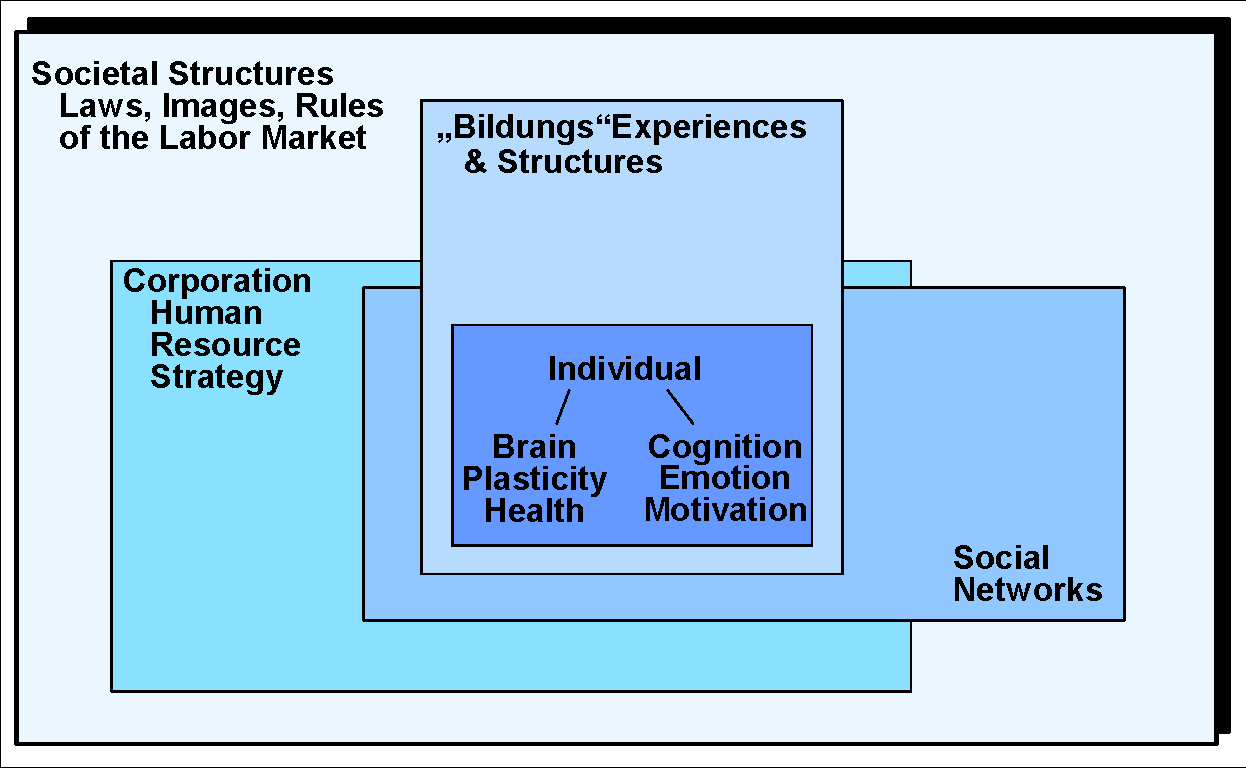
\includegraphics{deanUrsulaStaudingerIntro}}
   % \caption{Productive adult development at the Jacobs Center: A systemic approach (based on Staudinger, 2006).}
   % \label{fig:deanIntro}
  %\end{center}
%\end{figure}


\newpage
%The mechanic dimension refers to the fact that we all are biological beings with regard to our intelligence or cognition, our personality (motivation, emotion) and our social relations. This biological facet of our existence needs to be taken into account as facilitative and debilitating constraint to any intervention. At the same time, we are cultural and agentic beings, that is, there is a pragmatic dimension to human existence. Societal structures constrain and enable human development as well as individual choices and interpretations. 

%\begin{figure}[ht]
%  \begin{center}
%    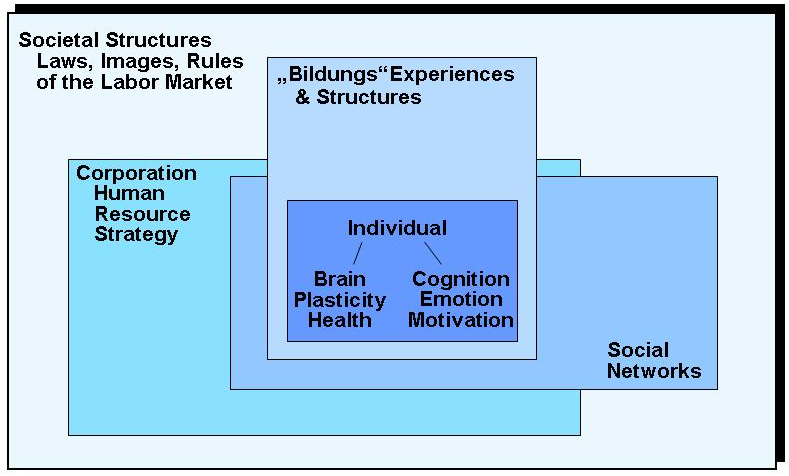
\includegraphics[width=7cm]{deanUrsulaStaudingerIntro.png}
%    \caption{Productive Adult Development at the Jacobs Center: A systemic approach (based on Staudinger, 2006).}\label{fig:deanIntro}
%   \end{center}
%\end{figure}



The developing individual is embedded in different important systems of influence that need to be kept in mind if the process of development is supposed to be productive. These systems are ``Bildungs'' experiences, social networks, the respective corporation with its approach to human resource development and finally the societal framework conditions such as the legal framework of work and education but also the images of aging and ``Bildung'' available in the public. In all these systems, changes have become necessary to accommodate the current transformative processes and enable successful lifelong learning and lifespan development. 


This systemic framework asks for multiple disciplines to be represented at the JCLL, such as Neuroscience and Human Performance, Lifespan Psychology, Health and Personality Psychology, Organizational Behavior (with a focus on learning in the work setting), Media and Communication Sciences (with a focus on images of aging, age-graded medial preferences and media competence), Business Administration, and Lifecourse Sociology and Economics.


The mutual \looseness=-1 dependencies of individual and social change are the focus of JCLL's joint research endeavors. For instance, the contribution of the Jacobs Center to the proposal of a Graduate School of the Social Sciences (BIGSSS) in the context of the Initiative for Excellence of the German Government (DFG / Wissenschaftsrat) lies exactly at the investigation of life-course and lifespan dynamics and their effect on individual and institutional or societal outcomes. Similarly, the interaction between the individual and the organization plays a central role in the first JCLL joint research proposal successful with the BMBF (Federal Ministry for Bildung and Research). In this project - that brings together all JCLL faculty under one common theme - we are interested in the matches and mismatches among employees' attitudes and competencies, the management strategies and work organization of the company as well the organizational climate with regard to the following domains: health promotion, training, images of aging, experience transfer, and adaptive competence. The central assumption is that individual as well as organizational outcomes (e.g., health, productivity) are best understood when taking into consideration the matches and mismatches between all possible combinations (Strategy - Climate, Climate - Employee, Employee - Strategy). Both a linear as well as a typological approach are considered as useful analytical tools. Five companies have agreed to participate. We will pursue a two-step sampling procedure: first we sample work units per company and second we sample individuals within each work unit. In order to keep the assessment protocol to a realistic length not all research domains will be assessed at each company. Rather, always two companies will have one domain in common. Thus, replication of findings across companies becomes possible. The research project, which will start in April 2007, is part of a program initiative by the BMBF revolving around innovative approaches to work security and health protection in the workplace. One of the results of this project will be a diagnostic toolbox for the identification of matches or mismatches in the domains of aging, learning, health, communication and adaptive capacity as well as application rules to be given to companies that want to work with the tool. 


Ursula M. Staudinger\\ 
Bremen, December 2006

%\cleardoublepage
\hyphenation{Life-long}
\section{Interdisciplinary Projects at the Jacobs Center} \shorttitle{Interdisciplinary Projects at the Jacobs Center}


\subsection{Demopass: Effects of Matches/ Mismatches between Aspects of Human and Social Capital, Corporate Strategy and Work Organization on the Physical and Mental Well-Being of Employees	}


%\enlargethispage*{2cm}

\paragraph{Research Team}
 Ursula M. Staudinger (Professor of Psychology), Ben Godde (Professor of Neuroscience), Heike Heidemeier (Postdoctoral fellow, Psychology), Brigitte Kudielka-W�st (Professor of Health Psychology), Christian Rossnagel (Professor of Organizational Behavior), Klaus Sch�mann (Professor of Sociology), Mireille Trautmann (Postdoctoral Fellow, Neuroscience), Claudia Voelcker-Rehage (Lecturer, Human Performance), Sven V�lpel (Professor of Business Administration), Stefan Baron (Doctoral Fellow, Sociology), Catherine Bowen (Doctoral Fellow, Psychology), Nicolas Feuerhahn (Doctoral Fellow, Health Psychology), Daniela Noethen (Doctoral Fellow, Business Administration).

\null
\textbf{Description of the project\smallskip}


Demographic change challenges management and corporate strategies as well as aging individuals. Companies face the challenge of staying innovative and productive with fewer young talents on the labor market, while individuals need to frequently update their skills and knowledge to maintain high levels of employability into (statutory) retirement age. Above all, employees' physical and psychological health is an invaluable resource and a precondition for the ability to maintain high levels of productivity throughout a career. Since the impact of demographic change on organizations is multifaceted, and demands action in several fields, an interdisciplinary perspective on productive aging is fitting.  All JCLL professors have worked together to contribute diverse perspectives within a joint research project. Project "Demopass" (from the German words "Demografie" and "Passung": demography and match/mismatch) examines matches and mismatches between several organizational levels (employees, management, and organizational strategies) that are crucial for understanding organizational outcomes, such as employee health and productivity. Moreover, the project emphasizes the important role that organizational climate (an aspect of an organization's social capital) plays in understanding organizational outcomes. Organizational climate communicates (implicit) expectations, values and incentives that may have a marked influence on actual behavior and the success of organizational strategies. The concept of matches and mismatches between three perspectives defines a reference framework that guides the work of five subprojects. 



\begin{figure}[htp]
 \begin{center}
    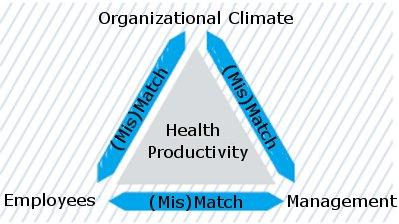
\includegraphics[natwidth=150, natheight=100]{fig1.jpg}
    \caption{Project Demopass}\label{fig:fig1}
   \end{center}
\end{figure}


%insert picture
%insert picture
%insert picture


\textbf{Research objectives}
 Project "Demopass" identifies five fields of action that are specifically relevant to tackling the challenges posed by demographic change in organizations: intergenerational knowledge transfer, training and on-the-job learning, images of aging in organizations, adaptive competences, and physical as well as psychological health. Exemplary research questions include the following: In order to establish successful knowledge management, employees' abilities to communicate and seek knowledge must match the expectations, resources and support provided by supervisors, as well as the forces implied in organizational climate. Specific consideration is given to intergenerational ("young to old" and "old to young") knowledge transfer. Similarly, images of aging and age-related organizational policies must be communicated in ways so that they match the beliefs of both employees and their supervisors. A company's "age climate" determines how others perceive older workers, and conveys whether they are esteemed members of the organization. Negative stereotyping may impair the motivation and productivity of older workers. This applies to self-views as well as the (assumed) views of others. Indeed, personal views and the views of others (supervisor beliefs or shared beliefs; i.e. "age climate") may positively or negatively complement or compensate for one other. A positive "age climate" may particularly help employees who tend to think negatively about their own aging to maintain effective self-regulation and higher levels of productivity. As a final example, the subproject on adaptive competencies examines meta-competencies that are highly relevant (in addition to specific skill or expertise) to meeting work demands. Again, an important assumption is that a match between perceived work demands, actual demands, and also employees' adaptive competencies contributes to an understanding of physical health and psychological well-being at work. Having to meet excessive demands may be as detrimental as insufficient challenge of skill and adaptive competencies. For the remaining two fields, training and health psychology, the same framework is applied to study matches and mismatches among the employees' competencies or attitudes, management support and strategies, and work climate.

\smallskip
 By studying a number of "paralleling" research questions, the project seeks to contribute to current understanding, while implementing an interdisciplinary approach. But the project also aims to communicate results so they are able to inform management practice. For that purpose, participating companies will receive feedback about their results. In addition, the project will assemble a toolbox for diagnosing matches and mismatches in organizations; this will be made available to companies which then can independently employ it. 


\paragraph{Outlook} 
  By the end of 2008, the project "Demopass" will have finished with data collection in five partnering companies. The project will then have collected questionnaire data and indicators of objective health from roughly 1500 employees and their supervisors. In addition, interviews with management representatives provide information about corporate and work strategies.  The research questions will be addressed empirically using a multi-level design, with individuals sampled from their work teams in order to ensure that they share the same social and physical work environment and climate. 

 Research results will begin to come to fruition in 2009. The project team also plans to carry out another round of data collection in order to validate the previously mentioned toolbox. This will be structured as a shortened version of the original questionnaire that will be tailored to address essential aspects of match/mismatch in the five action fields, and that will be designed to be applied by practitioners. In 2010 the project will attempt to scale up outreach both within the scientific community and with other relevant actors in private and public organizations. 

\paragraph{Grant} 
 Grant sponsorship was provided by the BMBF and the European Social Fund, "Effects of Matches/Mismatches between Aspects of Human and Social Capital, Corporate Strategy and Work Organization on the Physical and Mental Well-Being of Employees" (April, 2007). 

 Competency models are widely used by Human Resource (HR) practitioners in the selection, placement and development of employees. However, only little competency modeling research has been conducted, and the issue of age-related competency changes has hardly ever been addressed. In collaboration with Bosch Rexroth AG, we are developing a competency model that incorporates employees' age-related changes in ability and motivation factors. The model is intended to help identify HR development requirements in the mid-term (5 years).


 


\subsection{Mobility and Developmental Success }

%\enlargethispage*{2cm}

\paragraph{Research Team}
Ben Godde (Professor of Neuroscience), Klaus Sch�mann (Professor of Sociology), Ursula M. Staudinger (Professor of Psychology), Claudia Voelcker-Rehage (Lecturer, Human Performance), Heike Heidemeier (Postdoctoral fellow, Psychology)

\paragraph{Description of the project}
The aging and shrinking of the labor force in modern industrialized nations requires that companies and employees optimize their productivity across their life spans in order to both avoid jeopardizing economic success, and to enable individuals to successfully navigate through their extended life span. With increasing age there are certain gains and a greater number of losses that may interfere with the maintenance of individuals' productivity. Job mobility has become an increasingly important feature of the modern labor market. In addition, it may be that job mobility helps to compensate for some salient age-related declines, and thus can be considered a natural intervention to strengthening  productivity across life spans.




\paragraph{Research objectives}
Our main aim is to investigate the cumulative effects of voluntary job mobility on (productivity) and its interaction with individual developmental trajectories of adaptive competencies. We will focus on the large cohort of the so-called "baby boomers", who are currently entering into midlife and will constitute the future cohort of older workers.

Job mobility is defined as encompassing voluntary changes of the employer or company, as well job changes within a company. Extending traditional job mobility research, which has concentrated on single spells of mobility, we investigate (using sequence-analytical methods) the cumulative effects of job mobility. Adaptive competence comprises a cognitive as well as a personality component. In the first domain, our study deals with the capacity to adapt perceptual and motor functioning, as well as higher cognitive functions, to new or changing tasks or challenges. This takes into account the neurobiological mechanisms underlying such learning or adaptation processes.
The important dimension of adaptive competence in the domain of personality characteristics, on which we will focus, is the openness for new experiences, the readiness to take risks, and rigidity. As mediating and moderating variables we are interested in self-esteem, internal control beliefs, and accommodative as well as assimilative skills. Further, job-specific aspects like job commitment and job satisfaction play an important role.
We assume a strong relationship between both aspects of adaptive competencies on the one hand and job mobility on the other hand. We have two main hypotheses that may both be true. First, adaptive competences might strengthen job mobility, as adaptive workers are more able and ready to learn new tasks or to adapt to new working environments, and thus to take over new positions within their firm or in other firms. An adaptive personality, characterized by openness, may have a stronger motivation for changes and mobility.
Second, it may also be expected that voluntary job mobility, in turn, is able to increase adaptive competencies. Changing working tasks and experiences of job mobility "train" cognitive adaptivity, as well as adaptivity in the domain of personality, and thus avoid the usual age-related decline or even stimulate increases. On the other hand, routinized work and a lack of new challenges for several years might have negative impacts on adaptive competences; even they must be trained continuously.
Interested in cognitive as well as personality developmental processes, our multidisciplinary approach combining both is well suited not only to provide new evidence within the different domains of adaptivity, but also to investigate interactions between personality characteristics and underlying cognitive processes at the neural level. Moreover, we expect that findings in either domain allow predictions for the other.



\paragraph{Outlook} 
  In an important first empirical step, using secondary-analytical methods, we will recruit matching samples from the data of the German Socioeconomic Panel (SOEP).
These samples will differ with respect to their job mobility (high or low mobility) and - accounting for gender-specific careers - in terms of gender, resulting in a design with four different groups of participants. Groups have to be matched for confounding variables like job profile, social participation, health, qualification, life satisfaction, etc. Propensity Score Matching allows filtering persons with nearly identical characteristics differing only in respect to the specific factors of interest (job mobility and gender).
As the second empirical step, we will use these samples to investigate the two facets of adaptive competence development as antecedence and/or consequence of job mobility. 
In the domain of cognitive functions we will use neurophysiological and neuropsychological methods (functional MRI, behavioral tests) to examine adaptivity and learning abilities. Test parameters are, for example, the ability to adapt perception under fast switching conditions, the capacity to transfer learned skills to new situations, and the extent of cognitive flexibility and short-term cortical plasticity. 
In the domain of personality, questionnaires will be used to assess openness to new experience and rigidity, as well as internal control beliefs and accommodative/assimilative coping styles. Further, job-specific aspects like job commitment and job satisfaction are also investigated. 
Sample size is restricted by the SOEP data set itself but also by the applied methods. For the neurophysiological and -psychological tests a sample size of n=20 per group is intended. The total sample size to correlate personality characteristics with job mobility will be extended to all persons available in the dataset and willing to participate. First calculations suggest that we need to cumulate 4-5 birth cohorts (born between 1962 and 1966) in order to arrive at a final sample of 200 participants (50 in each group) that has complete information for 20 years; this is taking into account a 25% recruitment success rate. 
The current study suggests that it is useful to pool expertise from sociology, psychology and neuroscience in order to test whether voluntary job mobility may be considered a highly successful "natural" intervention when it comes to optimizing productivity across the life course. For this purpose, the study combines the unique longitudinal SOEP data set with behavioral and neuroscience methods, and utilizes the unique potential of secondary data analysis. The practical implications of the proposed study are obvious: given we find the alleged compensatory and facilitative effects of voluntary job mobility, this will send a strong signal to companies and employees alike to pursue the route of transforming traditionally stable work careers in Germany.


\paragraph{Grant} 
 This project is funded by Volkswagen Foundation.
 




 \cleardoublepage
\section{Discipline - specific Research Projects at the Jacobs Center} \shorttitle{Discipline-specific Research Projects at the Jacobs Center}


\subsection{Neuroscience and Human Performance }


%
\paragraph{Research Team}
Ben Godde (Professor of Neuroscience and Human Performance), Claudia Voelcker-Rehage (Lecturer, Human Performance), Mireille Trautmann (Postdoctoral Fellow, Neuroscience), Katja Dolge (Research Associate, Neuroscience).\newline \textbf {Former members}  Mikhail Babanin (Research Associate, Neuroscience), Laura Khil (Research Associate, Neuroscience), Johanna Stiehm (Research Associate, Human Performance), Alexander Kowanz (Research Associate, Human Performance).


\subsubsection{Promoting lifelong learning and development through detailed knowledge of underlying mechanisms}

Our research group is motivated by two central questions. First: How can lifelong learning and development be promoted? This means, how can we help people to gain optimal sensory, motor, and cognitive performance in different life phases and environments? Second: What are the neurobiological processes underlying lifelong learning and productive adult development, and how can these processes be modified and improved? For this purpose, our research focuses on identifying mechanisms underlying cortical plasticity and the structure/function relationships between cognitive, sensory, and motor performance and learning. The human brain remains plastic even at older age. However, plastic capacity declines with age. Thus, knowledge about the ability to facilitate plasticity is of high significance, particularly for the elderly learner. 

We address these research questions in several projects with a combination of neuroimaging, neuropsychology, physiology, and movement science. Although we examine human performance and its neurobiological basis during the whole life span, the relationships between sensory, motor and cognitive abilities, and the plastic-adaptive capacities of older adults are of particular interest for our research program. In this context, the research of our group is divided into the following main topics.


\subsubsection{Plastic-Adaptive Capacity of the Brain: Mechanisms, Effects of Age, Possible Interventions }

%\input{312}

Under this topic, we investigate the plastic adaptive capacity of the brain in order to understand basic mechanisms of plasticity and learning, as well as the effects of age. Based on experiments, possible interventions might be developed to improve learning and to interfere with age-related decline. In spite of the tremendous progress in brain imaging during the last two decades, which is now enabling detailed examination of brain activities related to complex cognitive functions, it is still rather difficult to unravel the underlying neuronal mechanisms and the relationships between neuronal activity, brain hemodynamics, and behavior. Thus, our research focuses on perception and motor action as more basic, but nevertheless well established, models of general brain functioning. Fields of research include vibrotactile perceptual learning, force control and force modulation, motor-cognitive dual-task performance, intermanual transfer of learned motor programs, and the sensory-motor coupling accompanying learning.

Within the sensory domain, we are mainly interested in plastic-adaptive competences related to tactile processing of younger and older adults. Using functional MRI and psychophysics, we investigate the cortical topography of tactile perception and the cortical mechanisms of perceptual learning. Within the motor domain, our focus is on upper extremity force control. Control of fine finger forces is an elementary component of movement production in many daily activities (e.g. dressing, eating, opening containers) and its assessment provides insight into movement control and coordination. A decline in force control is common in older adults. We examine age-related differences in force control, the practice // effect on force modulation, and age-related differences in dual-task performance. Besides force control, we are also interested in the intermanual transfer of learned motor programs.
Combining these two lines of research, we are going to focus on the interaction between motor and sensory performances. Sufficient sensorimotor functioning, in particular manual dexterity, is of major importance for independent living at old age. However, most older people suffer from a decline in their tactile and motor abilities. It is assumed that an important mechanism responsible for precise force control is tactile sensitivity. However, contradictory results also exist, and the neural control mechanisms responsible for precise manipulation of grasping forces are largely unknown. 
Using a protocol of high frequency tactile stimulation (tHFS), which has been shown to be very effective in inducing somatosensory cortical plasticity, our aim was: (a) to determine the effect of short-term tHFS on tactile and motor performance and (b) to examine tactile-motor interactions. Seventeen right-handed older adults (66-78 years) were randomly assigned to an experimental and a control group. Participants underwent a pre-test of tactile frequency and spatial discrimination performance, a test of manual dexterity, and a precision grip task with their left hands. They then received 30 minutes of tHFS on the tips of their left index fingers and thumbs, and performed a post-test. The control group received no stimulation. 



%insert figure

\begin{figure}[htp]
 \begin{center}
    \scalebox{0.5}{\includegraphics*[2.2in,4.3in][6.8in,6.8in]{figure1}}
    \caption{Left panel: Relative performance changes for the frequency discrimination task (a, FDT), spatial discrimination task (b, SDT), Purdue pegboard test (c, PBT), and force modulation task (d, FTT, RMSE) for the experimental (EG) and control group (CG) (means and standard errors). An asterisk marks significant performance changes different from zero (* p < .05). Note: Pre-to-post-test performance improvements are indicated by negative values for FDT, SDT, and FTT and by positive values for PBT. Right panel: Increased Beta-Power over the left sensorimotor cortex (marked by arrow) during the precision grip task was found after tHFS but not in the control group.  }\label{fig:fig2}
   \end{center}
\end{figure}

%insert figure

%insert figure

%insert figure


Results indicated an improvement in frequency and spatial discrimination performance in the experimental group but not in the control group (cf. Figure 1). For the precision grip task, however, improved performance, as found for the control group, did not occur for the experimental group. For the manual dexterity task, no effect was found either for the experimental or for the control group. Our data indicate that tHFS might influence tactile performance positively in older adults. Although it still remains open whether improved tactile function is functionally unimportant for a pure grip task as used in the current studies, or whether tHFS-induced cortical changes result in no improvement in the precision grip, our results give further evidence to the notion of an interrelation between sensory and motor performances.


\subsubsection{Effects of Cardiovascular and Motor Fitness on Cognitive 	Performance and Well-Being in Older Adults }

%\input{313}

Physical fitness is assumed to preserve cognitive functioning and psychological well-being in older adults. More and more animal and human studies stress the importance of a physically active lifestyle for successful aging (i.e. delayed cognitive decline, improved physiological and psychological health, etc.). However, the mechanisms, the dose-response relationship, and also the effects of different types of exercise are not well understood. This second area of research, which follows an interdisciplinary view on human performance that comprises motor, neurophysiological and psychological expertise and methods, deals with the role of aerobic and non-aerobic motor exercise on cognitive performance and well-being across the lifespan.

In a one-year longitudinal study, we investigated the effects of different types of physical activity on cognitive performance and well-being in older adults. 116 older men and women (61-79 years; M = 68.74; SD= 3.50) participated in our study. All participants were recruited from a member register of the German health insurance company DAK and were randomly assigned to one of three intervention groups (endurance training, strength training, or relaxation and stretching). Training groups met three times a week for 12 months. Before the start of the training program, every three months during the intervention, as well as 12 months after its conclusion, the participants spent two days in the lab for extended testing of cognitive and motor abilities, emotion regulation, and subjective well-being. In addition, participants were examined with functional MRI in the beginning, in the middle, and at the end of the intervention study, in order to visualize changes in brain processes during performance of cognitive, motor, and emotional tasks.

For a first cross-sectional analysis of the relationship between motor status and cognitive performances we calculated performance indices for primary intellectual abilities like executive control and perceptual speed (measured by a flanker task, a visual search task, a picture identification task, and an n-back task as memory task) as well as, based on an extended battery of motor tests and spirometric measures, motor status in respect to physical (cardiovascular fitness and strength) and motor fitness (balance, coordination, speed, flexibility). Both behavioral and imaging data revealed differential effects of physical and motor fitness on cognitive performance and related brain processes. At the behavioral level, physical fitness was mainly related to executive control processes (measured with the flanker and n-back task), whereas motor fitness showed a significant association with both the executive control and the perceptual speed tasks (measured with the identical picture and visual search task, cf. figure 2). 

Altogether, our behavioral results support the idea that fitness is differently associated with indicators of fluid intelligence such as perceptual speed and executive control. Imaging data for response competition (flanker task) also indicated that a high physical fitness level might be positively related to resources available for executive control processes. In particular, the right IFG has been shown to be important for interference control during the flanker task, and was activated more strongly in the physically fit participants. A high level of motor fitness, on the contrary, seems to require less effort exerted for the inhibition of distracting information and for motor preparation; this might cause more effective processing and integration of visuo-spatial information. This was indicated by less frontal but stronger and focal sensorimotor and parietal activation found for high versus low motor fit participants. Herewith, we were able to add important insights to the topic of brain aging. Based on the high inter-individual variability in age-related changes in cognition, fitness, and brain activation patterns, it seems useful to tailor preventive physical training interventions accordingly. Analysis of the longitudinal data is underway to test the specific cognitive and neurophysiological effects of a motor-fitness training program as compared to a classical cardiovascular training.


\subsubsection{Mobility and Developmental benefit }

%\input{314}

In a third line of research, we are interested in the effects of working life experiences on the cognitive functioning and plastic-adaptive capacity of middle-aged individuals (40-50 years of age). Within the joint project "Mobility and Developmental Benefit" we pursue the question: does job-related mobility have a cumulative effect on the development of cognitive and personality adaptivity (see Mobility project).

\subsubsection{DemoPass Project}

%\input{315}

Finally, the plastic-adaptive capacities of the adult and aging brain are of particular importance for the aging work force. Combining our expertise in the above mentioned fields of research as a part of joint JCLL efforts, we developed the aim to establish measures of older workers' adaptivity in the sensory, motor, and cognitive domains and to relate their adaptive capabilities to the demands of the work place. From the results, we will be able to identify mismatches between demands of the work place and individual preconditions. We assume that these mismatches might be used as predictors of low productivity or employee health problems (see DemoPass project). 

\subsubsection{Collaborators }

%\input{316}

\begin{itemize}
\item University of Bielefeld \\ Department of Sports Science \\ Prof. Dr. Klaus Willimczik.
\item University of Bremen\\ Movement Science and Training, \\Sports Science\\ Dr. Monika Fikus.
\item University of Bremen \\ Interdisciplinary Center for\\ Cognitive Sciences \\ Prof. Dr. Manfred Herrmann.
\item University of Bremen \\ Interdisciplinary Center for\\ Cognitive Sciences \\ Prof. Dr. Manfred Fahle.
\item University of T�bingen, MEG-Center \\ PD Dr. Christoph Braun.
\item Ruhr-University Bochum\\ Institute for Neuroinformatics\\ PD Dr. Hubert Dinse.
\item International School for Advanced Studies, Trieste, Italy\\  Cognitive Neuroscience Sector \\ Prof. Mathew E. Diamond, PhD.
\item Lerner Research Institute, USA\\  Department of Biomedical Engineering,\\ Cleveland Clinic Foundation\\ Jay L. Alberts, PhD.
\item Jacobs University, SES \\ Prof. Dr. Claus Hilgetag.
\item Jacobs University, JCLL \\ Prof. Dr. Ursula M. Staudinger.
\item University of Tulsa, Psychology Department\\ Nonconscious Information \\ Processing Laboratory\\ Pawel Lewicki, PhD.
\item Humboldt University Berlin\\ Department of Movement and\\ Training Science\\ Dr. Henning Budde.
\item University of Hamburg\\ Department of Human Movement\\ Prof. Dr. Volker Lippens.
\end{itemize}


\subsubsection{Other Professional Activities }

%\input{317}

Claudia Voelcker-Rehage is Junior Fellow of the Leopoldina-Acatech-Workgroup "Chancen und Probleme einer alternden Gesellschaft: Die Welt der Arbeit und des lebenslangen Lernens" (since 2005).

\paragraph{Ad-hoc Reviews}
\textbf{Godde:}
Journal of Cognitive Neuroscience, Psychophysiology, Neuroscience and Biobehavioral Reviews, Journal of Neurophysiology, Journal of Neuroscience Methods, The Quarterly Journal of Experimental Psychology.

\textbf{Voelcker-Rehage:}
Deutsche Zeitschrift f�r Sportmedizin, European Review on Aging and Physical Activity, Experimental Brain Research, Medical Science Monitor, Journal of Gerontology: Psychological Science, Psychological Reports Perceptual and Motor Skills, Zeitschrift f�r Sportpsychologie


\subsubsection{Publications }

%\input{318}


\subsection{ Stress and Health at Work}

%
\paragraph{}

\begin{flushleft}
\textbf{Research Team}
\end{flushleft}

Christian Stamov Ro�nagel (Professor of Organizational Behavior), Melanie Schulz (Doctoral Fellow; since 02/2007), Jennifer Bittner (Postdoctoral Fellow; since 12/2008).

\paragraph{}
Workers bring to their workplace a set of personal resources, often referred to as KSAOs (i.e. knowledge, skills, abilities and other characteristics); examples include motives, personality and values. Jobs offer a variety of job resources; examples include task complexity, leader-member exchange, and organizational climate. Both types of resources interact in shaping organizational behavior. Two workers equipped with the same personal resources will show quite different work behaviors depending on the availability of job resources. Similarly, even under maximally supportive job conditions, two workers will fair quite differently to the extent that they are endowed with different personal resources. 

\paragraph{}
Human development across the lifespan is a major determinant of this interaction, impinging differentially on different kinds of personal and job resources. While availability is likely to decrease for some resources (e.g., certain cognitive abilities) and to increase for other resources (e.g., expertise), utility is likely to change for still other resources (e.g., task variety). In sum, losses in some resources coupled with stability or growth in other resources lead to systematic patterns of qualitative changes in work behaviors, and it is these patterns that we are interested in. 

\paragraph{}
We conduct much of our research in collaboration with personnel decision-makers from major companies such as Deutsche Bank, EnBW, and OTTO Group. From the perspective of Dynamic Human Resource Management (D-HRM, see Staudinger, Ro�nagel \& Voelpel, 2008) we emphasize the need for integrated action on five action fields. The central assumption of D-HRM is that workers and jobs alike significantly and systematically change across work life. This alters the fit between workers and their jobs, which has been shown to be an important determinant of job satisfaction and commitment. One of the objectives of Dynamic HRM is to provide tools for proactive fit management in order to enable sustainable work conditions across work life. Developing research designs in close exchange with practitioners has helped raise both academically and practically interesting research questions. Given the rigor we bring into our research, such exchange increases the validity and generalizability of our findings.

\paragraph{}
Much of the research on older workers' training and development participation has focused on the role of KSAO and training characteristics as determinants of training participation and outcomes; much less evidence is available on the influence of organizational determinants (e.g., training climate). We have therefore taken the demopass project (see 2.1) as an opportunity to extend the well-established person-environment fit perspective to T\&D issues. Building on preliminary findings that individual "fit style" (e.g., emphasizing person-organization vs. person-job fit) may change with age, we have set up the T\&D part of the demopass survey so that the relative roles of supervisor and team support, and a company's training climate for predicting training participation can be investigated.

\subsubsection{Age Differences in Workplace Learning }


\begin{flushleft}
\textbf{Research Program} 
\end{flushleft}

Informal learning is said to be developing into an increasingly important part of companies' training and development (T\&D) activities. Such learning takes places outside traditional courses and may occur as participation in quality circles, mentoring programs, self-organized study, or simply as "learning by doing". Informal learning shares many features of self-regulated learning; thus we explore informal learning in terms of a learning competency arising from the interplay of cognitive (learning strategies), meta-cognitive (monitoring), and motivational (e.g., epistemic belief) dimensions. Our research is aimed at identifying the competency dimensions most relevant for predicting learning success.

\begin{figure}[htb]
  \begin{center}
    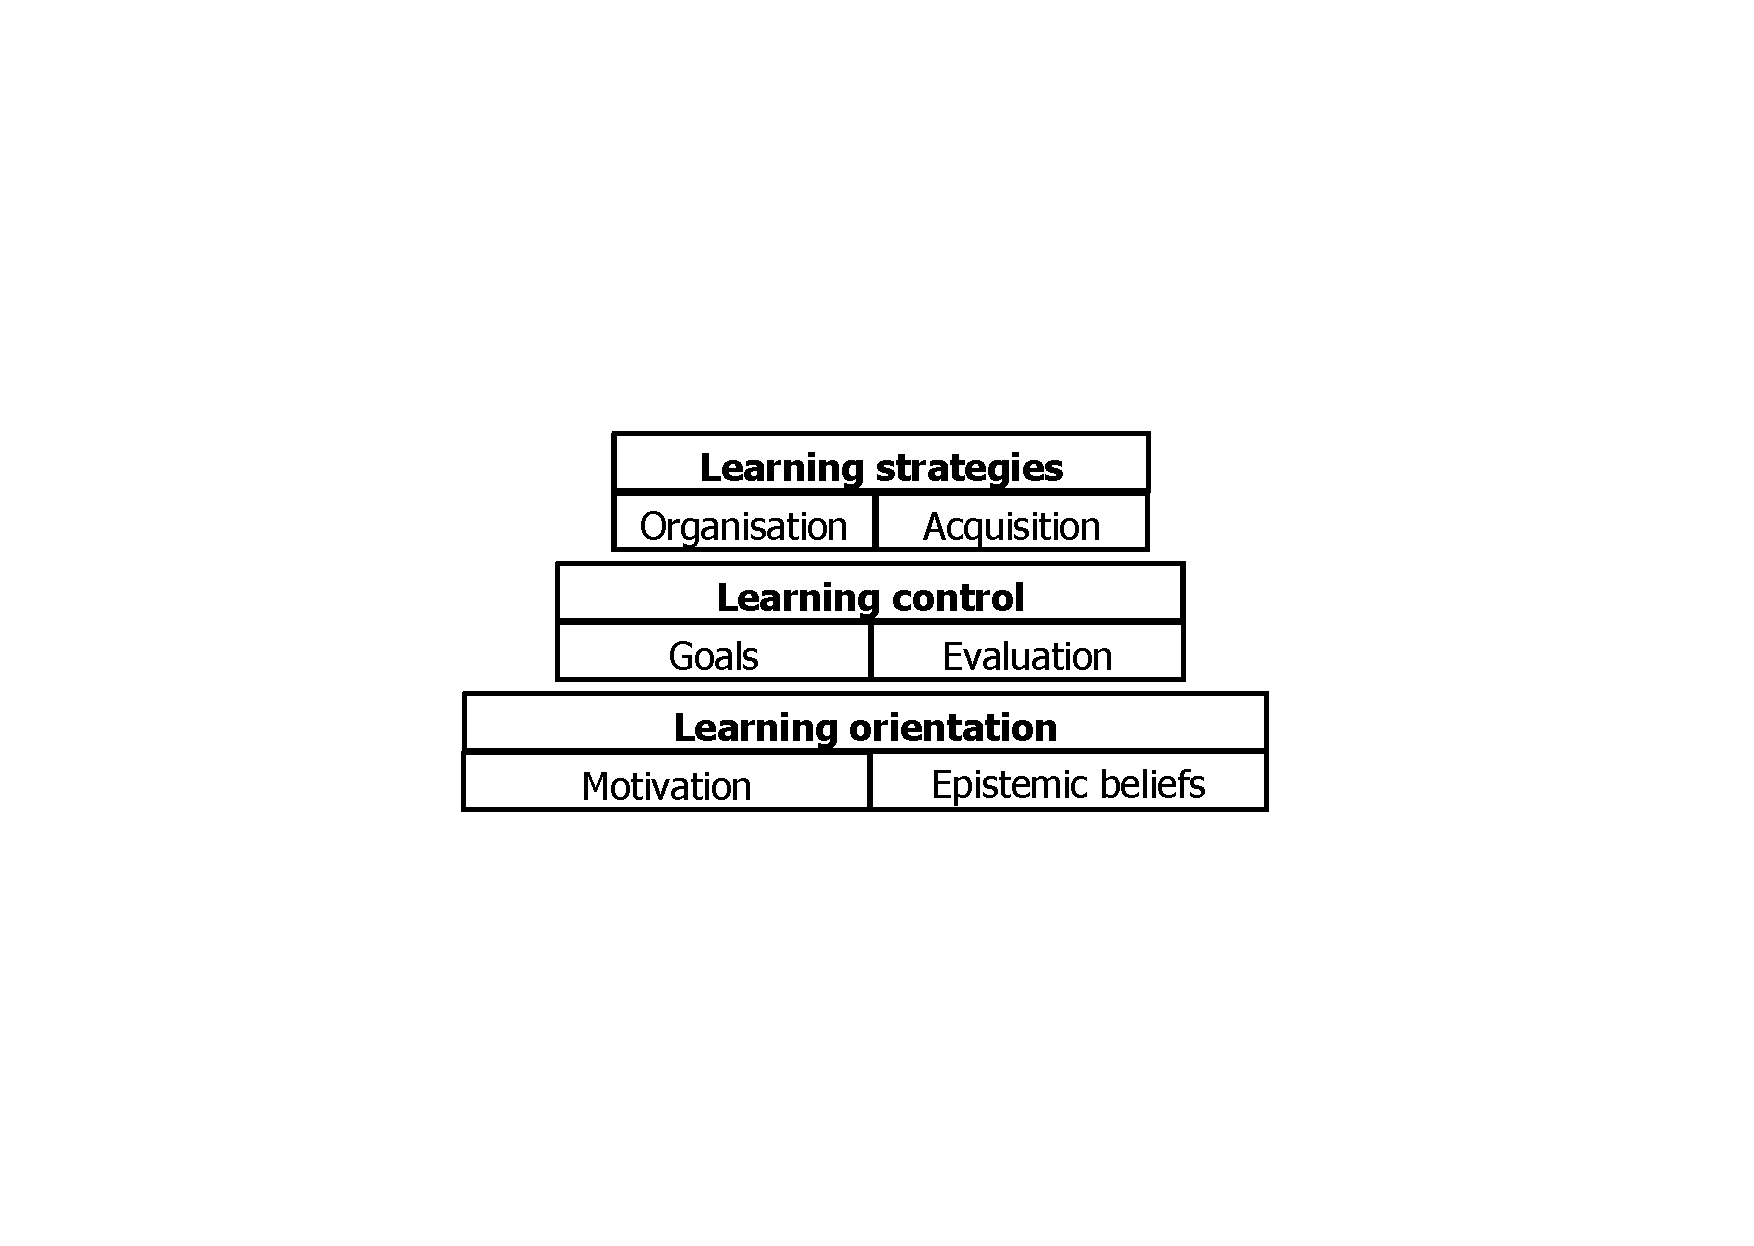
\includegraphics[width=0.5\textwidth,height=8cm]{RR2008CSRImage.pdf}
    \caption{Levels and central constructs of learning competency.}
  \end{center}
\end{figure}

\begin{flushleft}
\textbf{Research Highlights 2007/2008}
\end{flushleft}

We began with employee surveys assessing the interplay of meta-cognitive and motivational variables, and the influence of organizational variables (e.g., T\&D climate, learning opportunities at work) on learning competency. Results indicated that older workers showed learning competency decreases from declines in memory self-efficacy (MSE) rather than as a function of biological age. As such declines are particularly likely in organizations that offer few learning opportunities, and that fail to encourage continuous T\&D participation, older workers are more likely than their younger colleagues to experience MSE decline; it may thus be seen as a secondary age effect. We follow up on these findings in laboratory research investigating the interplay of age, MSE, and task difficulty in cognitive resource allocation to self-regulated learning tasks in an e-learning environment. Intervention studies follow naturally from this approach, and thus they form a third focus of our research. We have started designing "learning competency workshops" that seek to enhance learning performance by training goal-setting and monitoring skills.


\subsubsection{Age-Related Changes in Work Motivation }


\begin{flushleft}
\textbf{Research Program}
\end{flushleft}


Given decreasing numbers of young workforce entrants, the successful retention of older workers is of high importance for many organizations; this requires a profound understanding of older workers' motivation. While aging, more often than not, is perceived to involve inevitable decline in motivation, we posit that age-related changes in work motivation might be conceptualized as outcomes of active regulation. Rather than passively responding to personal (e.g., capability declines) and environmental (e.g., altered work demands) changes, older workers actively adapt to these changes. As a result, work motivation becomes more task-specific; the influence of work context on motivation changes both quantitatively and qualitatively and leads to developing an individual motivational profile (Stamov Ro�nagel, in press).

\paragraph{}
In co-operation with various companies, we develop within this framework tools for motivation diagnostics and interventions. We seek to identify specific areas of age-related increases and decreases. Beyond academic interest, conceptualizing age-related changes in motivation as an outcome of active regulation might provide human resource professionals with more opportunities for motivation interventions. For instance, giving older workers higher degrees of job control might help fulfill their needs for job customization, and may enable them to allocate effort in line with their motivational profile. In a similar vein, discussing and "teaching" motivational regulation strategies might help equip older workers with skills to successfully cope with age-related capability changes and changing job demands. Finally, research into motivation profiles might increase the effectiveness and efficiency of motivational interventions, and might be fruitful for building (age-diverse) teams.

\paragraph{}
\begin{flushleft}
\textbf{Research Highlights 2007/2008}
\end{flushleft}

In a recently completed survey, we asked 312 workers (ages 18-65) from a company to rate how motivated they were for their work in general and for tasks emphasizing collaboration with colleagues, demonstration of one's knowledge and skills, learning new skills or knowledge, leading others, working autonomously, and passing to colleagues one's knowledge and experience, respectively. Moreover, to assess needs-supplies fit, participants indicated whether they felt they were given sufficient opportunities to work on each of these task types. We found that the motivation patterns as defined by the six aforementioned types of tasks differed as a function of age. Most importantly, older workers showed higher levels of motivation than their younger colleagues on the "people tasks" involving passing on knowledge and experience and leading others. Independent of age, the overall level of motivation was higher for participants who reported good fit, that is, older workers who reported high needs-supplies fit rated their overall motivation on a comparable level than their younger colleagues. Also, high levels of fit were associated with positive affect at work, indicating that task-specific motivation regulation might be a useful strategy of affect regulation.


\subsubsection{Older Workers' Cognitive Resources for Innovation Behavior }



Most recently, we have embarked on innovation behavior research, which will be funded by a Volkswagen Foundation grant until 2011. Similar to the situation with workplace learning and motivation research, older workers have been somewhat neglected in this field. Although the demand for innovation increases in the wake of technological change and globalization, and although a growing number of older workers will be involved in innovation-related work roles, little research has dealt with the question how age might affect innovation behavior.

\paragraph{} 
Our research focuses on the motivation-cognition interface. We assume that while aging might objectively affect older workers' cognitive innovation resources, workers will strive to compensate for declining resources availability if such compensation is supported by the organization. Routinization, a facet of expertise, is a resource of particular interest in this regard. It frees up cognitive capacity that in an innovation-supporting environment might be directed towards recognizing innovation potentials and developing implementation strategies. In a less supportive environment, however, routinization may be married with unproductive routine. Like for our workplace learning and motivation research, we develop a combination of quantitative survey and experimental methods to investigate the role of personal cognitive resources.


\subsubsection{Collaborators }

%\input{326}
\begin{itemize}
\item University of Heidelberg; \\Sonja Bausch.
\item University of Dortmund;\\ Michael Falkenstein.
\item University of Oldenburg;\\ Prof. Dr. Barbara Moschner.
\item University of Passau;\\ Prof. Dr. Franz Lehner.
\item Portland State University;\\ Prof. Dr. Pamela Tierney.
\item Bremen-Nord Hospital.
\item Deutsche Bank.
\item EnBW.
\item HeidelbergCement.
\item OTTO Group.
\end{itemize}


\subsubsection{Other Professional Activities }


\textit{Ad-hoc reviews:}
Applied Psychology: An International Review, European Journal of Personality, Journal of Behavioural Sciences, Zeitschrift f�r Personalpsychologie, Zeitschrift f�r Sozialpsychologie. \\

\textit{Boards 2007/2008}

\begin{itemize}
\item EU Commission. Member of the Board of Judges, \textit{European Union eInclusion Awards.}
\item Federal Institute of Occupational Health and Safety (BAuA), Advisory Board Member of the PFIFF project.
\end{itemize}

\subsubsection{Publications }

\begin{itemize}

\item Stamov Ro�nagel, C. (in press). Motivationsregulation �lterer Besch�ftigter. In K. Brauer \& G. Korge, editor, \textit{Perspektive 50plus? Theoretische und Praktische Ans�tze zur regionalen Arbeitsmarktf�rderung �lterer.} Wiesbaden: Verlag f�r Sozialwissenschaften. 

\item Stamov Ro�nagel, C. (in press). Arbeitsmotivation �ber die Lebensspanne: Aktive Regulation statt passiven Abbaus. In J. Kocka, M. Kohli, \& W. Streeck (Hrsg.), \textit{Altern, Familie, Zivilgesellschaft und Politik.} Stuttgart: Wissenschaftliche Verlagsgesellschaft.

\item Stamov Ro�nagel, C. (in press). Was H�nschen nicht lernt...? Folgen der Altersselektion bei Weiterbildungskonzepten. In K. Brauer \& W. Clemens (Hrsg.).\textit{ Zu Alt? Zur Theorie des Ageism und zur Empirie der Altersdiskriminierung auf Arbeitsm�rkten}. Wiesbaden: Verlag f�r Sozialwissenschaften.

\item Gotoh, F., Kikuchi, T., \& Stamov Ro�nagel, C. (2008). Emotional Interference in Enumeration: A Working Memory Perspective. \textit{Psychology Science Quarterly}, 50 (4), 526-537.

\item Stamov Ro�nagel, C. (2008). Motivationsregulation �lterer Besch�ftigter. In K. Brauer \& G. Korge (Eds.), \textit{Perspektive 50plus? Theoretische und Praktische Ans�tze zur regionalen Arbeitsmarktf�rderung �lterer} (p. 71-86). Wiesbaden: Verlag f�r Sozialwissenschaften.

\item Stamov Ro�nagel, C. (2008). \textit{Mythos "Alter Mitarbeiter": Lernkompetenz jenseits der 40}? Weinheim: Beltz PVU.

\item Stamov Ro�nagel, C., Picard, M.A., \& Voelpel, S. (2008). Weiterbildung jenseits der 40. \textit{Personal}, 36-38.

\item Lehner, F. \& Ro�nagel, C. (2008). iVideo - An Easy-to-use Authoring Tool for Interactive E-Learning Videos. In Luca, J. \& Weippl, E.R. editors, \textit{Proceedings of ED-MEDIA 2008 - World Conference on Educational Multimedia, Hypermedia \& Telecommunications} (5373 - 5378). Chesapeake, VA: AACE. 

\item Staudinger, U. M., Ro�nagel, C., \& V�lpel, S. (2008). Strategische Personalentwicklung und demographischer Wandel - eine interdisziplin�re Perspektive. In K. Schwuchow \& J. Gutmann, J., editors, \textit{Jahrbuch Personalentwicklung 2008 - Ausbildung, Weiterbildung, Management Development} (295-304). M�nchen: Luchterhand.

\item Ro�nagel, C. \& Schulz, M. (2007). Besch�ftigungsf�higkeit erfahrener Mitarbeiter. sichern - welche Rolle spielt die betriebliche Weiterbildung Ergebnisse einer Befragung von Unternehmen in Ostwestfalen-Lippe. G�tersloh: Bertelsmann.

\item Ro�nagel, C. \& Voelpel, S. (2007). Qualifizierung �lterer Mitarbeiter: Keine Einheitsweiterbildung. \textit{Persorama}, 35, 24-29.

\end{itemize}

\subsection{The Plasticity of Adult Development: Lifespan Perspectives}


\subsubsection{Contexts Facilitating Adult Development and Aging}

%insert

\subsubsection{Physical and Motor Fitness as Facilitators of Cognitive and Emotional Plasticity }

%insert

\subsubsection{Developmental Regulation and Self-Regulation as Facilitators of Adult Development and Aging}

%insert

\subsubsection{Two Types of Positive Personality Development: Adjustment and Growth }

\paragraph{}
\begin{flushleft}
\textbf{Research Program}
\end{flushleft}

Does personality stay stable after young adulthood or is there continued change throughout middle and later adulthood? For decades, this question has caused heated debate. In recent years, a consensus has emerged based on contemporary cross-cultural as well as longitudinal evidence. This consensus confirms that indeed there is personality change in middle and later adulthood. Many authors have labeled this change, personality maturation or growth. In somewhat simplified terms the observed pattern is as follows: Neuroticism declines, conscientiousness and agreeableness increase. At the same time it has been argued that this pattern of personality change is the result of coping with the developmental tasks of adulthood and thus increased adjustment. In this research area, we are interested in exploring the different ways of operationalizing adjustment and growth, and also finding out about their developmental dynamics. 

\paragraph{}
\begin{flushleft}
\textbf{Research Highlihts 2007/2008}
\end{flushleft}

Our two goals were to develop and validate a performance measure of personal wisdom (PW), and to examine age differences. Based on the Berlin wisdom paradigm and growth theories of personality, five criteria of PW were developed. A sample of 83 younger (20-40) and 78 older adults (60-80) thought aloud about a PW task. Transcribed answers were rated. Validity was established with regard to indicators of personality growth, subjective well-being, intelligence, critical life events, as well as general wisdom (GW; see Fig. 14). As expected, no age differences were obtained on the basic criteria and negative age differences were found on the meta-criteria indexing PW. Fluid intelligence and openness to new experience partially mediated these differences. It is argued that on average and for current cohorts, age-related changes in psychological functioning may act as hindrances to PW.

\begin{figure}[htb]
  \begin{center}
    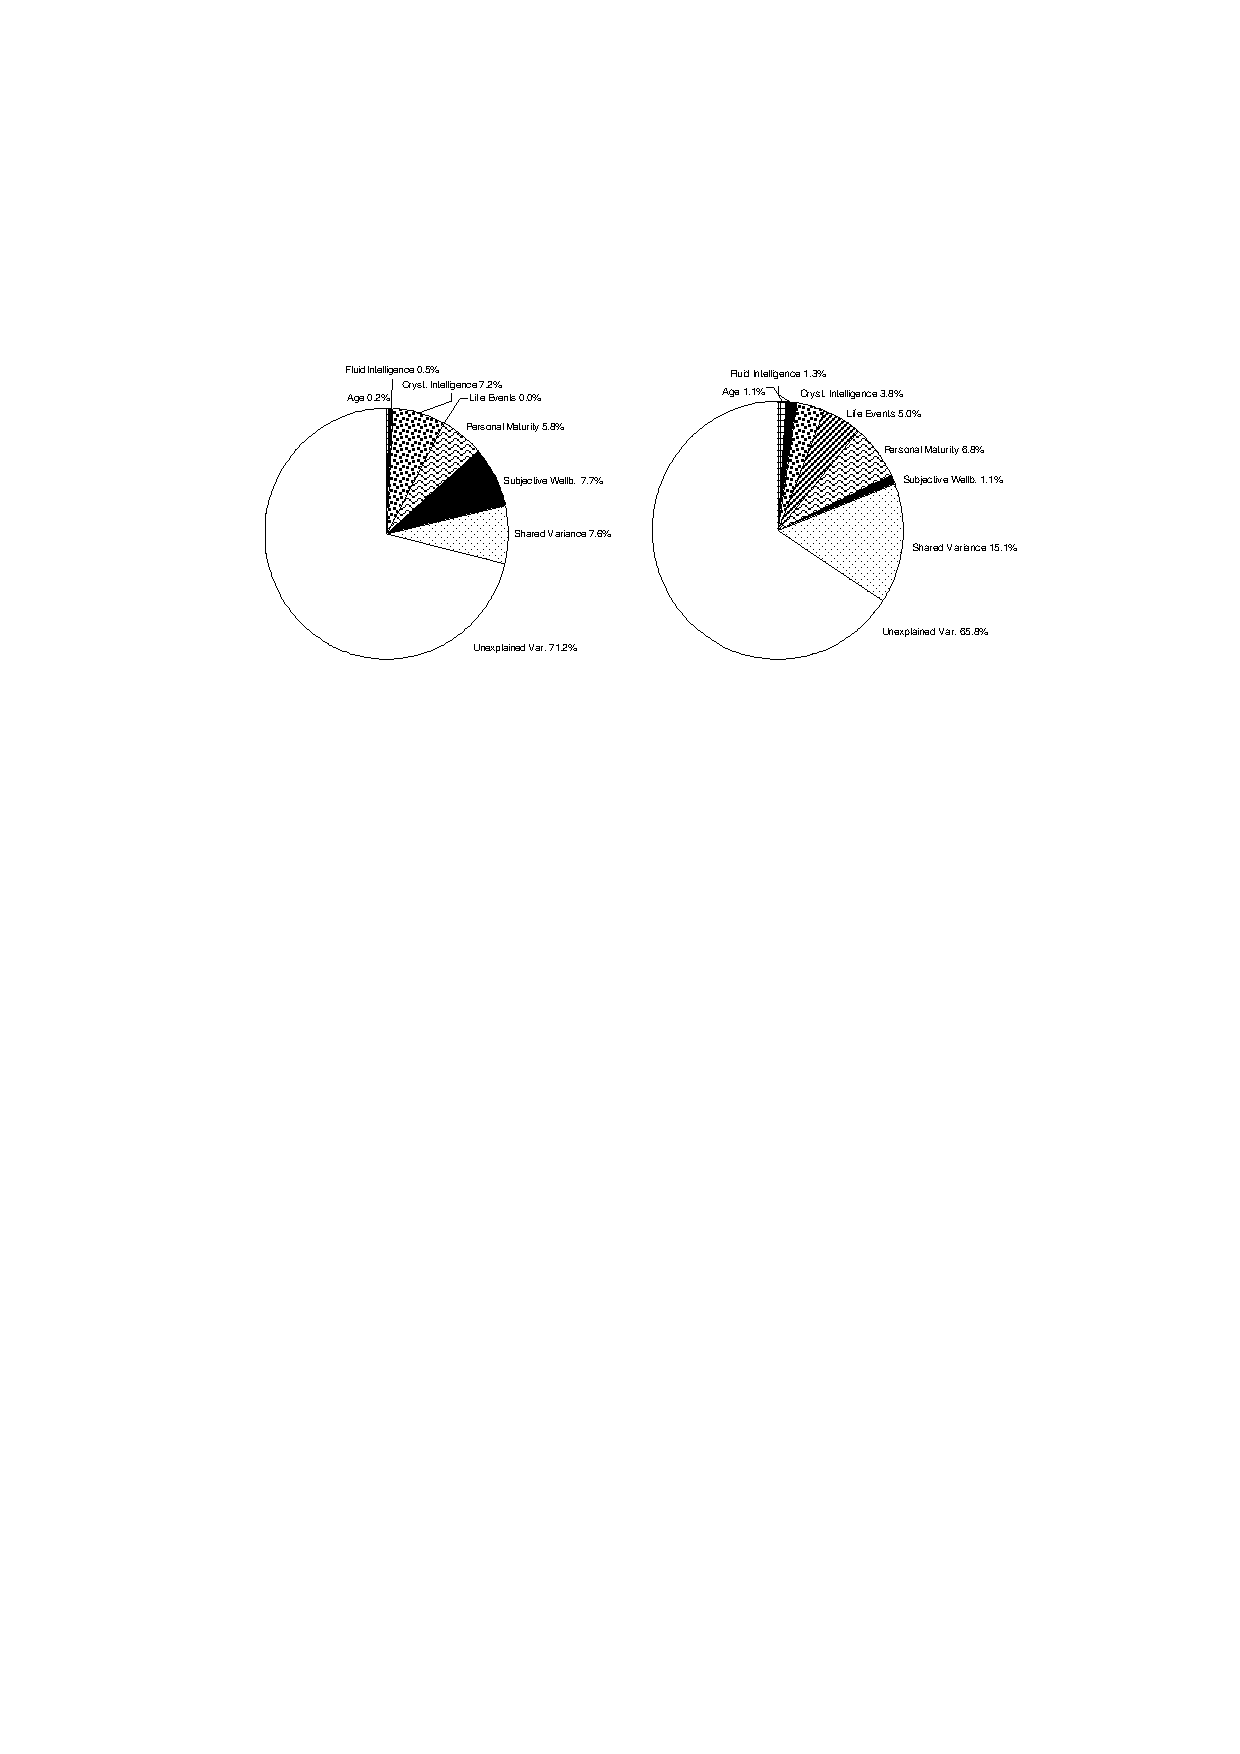
\includegraphics[width=0.5\textwidth,height=5.5cm]{fig14.pdf}
    \caption{Predictive validity of two wisdom measures (results of commonality analysis; Mickler \& Staudinger, 2008)}
  \end{center}
\end{figure}

\subsubsection{Collaborations}

\begin{itemize}

\item Brandeis University; Prof. Margie Lachman, PhD
\item Humboldt University, Berlin�; Dr. Charlotte Mickler
\item Jacobs University, JCLL�; Prof. Dr. Ben Godde
\item Jacobs University, JCLL�; Prof. Dr. Klaus Sch�mann
\item Jacobs University, JCLL�; Dr. Claudia Voelcker-Rehage
\item Max Planck Institute for Human Development, Berlin; Prof. Dr. Ulman Lindenberger  
\item Stanford University; Prof. Laura Carstensen, PhD
\item University of Florida, Gainsville, FLA; Prof. Manfred Diehl, PhD
\item University of Frankfurt; Prof. Dr. Tilmann Habermas
\item University of Klagenfurt;Prof. Dr. Judith Gl�ck
\item University of Heidelberg�; Prof. Dr. Hans-Werner Wahl
\item University of Hildesheim; Prof. Dr. Werner Greve
\item University of Michigan�; Prof. Patricia Reuter-Lorenz, PhD
\end{itemize}

\subsubsection{Other Professional Activities}

\begin{itemize}

\item Alexander von Humboldt Stiftung, Member of Selection Committee
\item Berlin-Institut f�r Bev�lkerung und Entwicklung, Member of the Advisory Board 
\item German Center for Gerontology, DZA, Member of the Scientific Board
\item German Psychological Society, President
\item Joint Academy Network "Aging in Germany" (Leopoldina, acatech), Co-Speaker
\item Leopoldina National Academy of Sciences, Vice President
\item Margret M. and Paul B. Baltes Foundation, Chair 
\item Max Planck International Research Network on Aging (MAXNET Aging), Senior Fellow 

\end{itemize}



\subsection{A Lifespan Perspective on Organizational Behavior}



\paragraph{}

\begin{flushleft}
\textbf{Research Team}
\end{flushleft}

Christian Stamov Ro�nagel (Professor of Organizational Behavior), Melanie Schulz (Doctoral Fellow; since 02/2007), Jennifer Bittner (Postdoctoral Fellow; since 12/2008).

\paragraph{}
Workers bring to their workplace a set of personal resources, often referred to as KSAOs (i.e. knowledge, skills, abilities and other characteristics); examples include motives, personality and values. Jobs offer a variety of job resources; examples include task complexity, leader-member exchange, and organizational climate. Both types of resources interact in shaping organizational behavior. Two workers equipped with the same personal resources will show quite different work behaviors depending on the availability of job resources. Similarly, even under maximally supportive job conditions, two workers will fair quite differently to the extent that they are endowed with different personal resources. 

\paragraph{}
Human development across the lifespan is a major determinant of this interaction, impinging differentially on different kinds of personal and job resources. While availability is likely to decrease for some resources (e.g., certain cognitive abilities) and to increase for other resources (e.g., expertise), utility is likely to change for still other resources (e.g., task variety). In sum, losses in some resources coupled with stability or growth in other resources lead to systematic patterns of qualitative changes in work behaviors, and it is these patterns that we are interested in. 

\paragraph{}
We conduct much of our research in collaboration with personnel decision-makers from major companies such as Deutsche Bank, EnBW, and OTTO Group. From the perspective of Dynamic Human Resource Management (D-HRM, see Staudinger, Ro�nagel \& Voelpel, 2008) we emphasize the need for integrated action on five action fields. The central assumption of D-HRM is that workers and jobs alike significantly and systematically change across work life. This alters the fit between workers and their jobs, which has been shown to be an important determinant of job satisfaction and commitment. One of the objectives of Dynamic HRM is to provide tools for proactive fit management in order to enable sustainable work conditions across work life. Developing research designs in close exchange with practitioners has helped raise both academically and practically interesting research questions. Given the rigor we bring into our research, such exchange increases the validity and generalizability of our findings.

\paragraph{}
Much of the research on older workers' training and development participation has focused on the role of KSAO and training characteristics as determinants of training participation and outcomes; much less evidence is available on the influence of organizational determinants (e.g., training climate). We have therefore taken the demopass project (see 2.1) as an opportunity to extend the well-established person-environment fit perspective to T\&D issues. Building on preliminary findings that individual "fit style" (e.g., emphasizing person-organization vs. person-job fit) may change with age, we have set up the T\&D part of the demopass survey so that the relative roles of supervisor and team support, and a company's training climate for predicting training participation can be investigated.

\subsubsection{Age Differences in Workplace Learning }


\begin{flushleft}
\textbf{Research Program} 
\end{flushleft}

Informal learning is said to be developing into an increasingly important part of companies' training and development (T\&D) activities. Such learning takes places outside traditional courses and may occur as participation in quality circles, mentoring programs, self-organized study, or simply as "learning by doing". Informal learning shares many features of self-regulated learning; thus we explore informal learning in terms of a learning competency arising from the interplay of cognitive (learning strategies), meta-cognitive (monitoring), and motivational (e.g., epistemic belief) dimensions. Our research is aimed at identifying the competency dimensions most relevant for predicting learning success.

\begin{figure}[htb]
  \begin{center}
    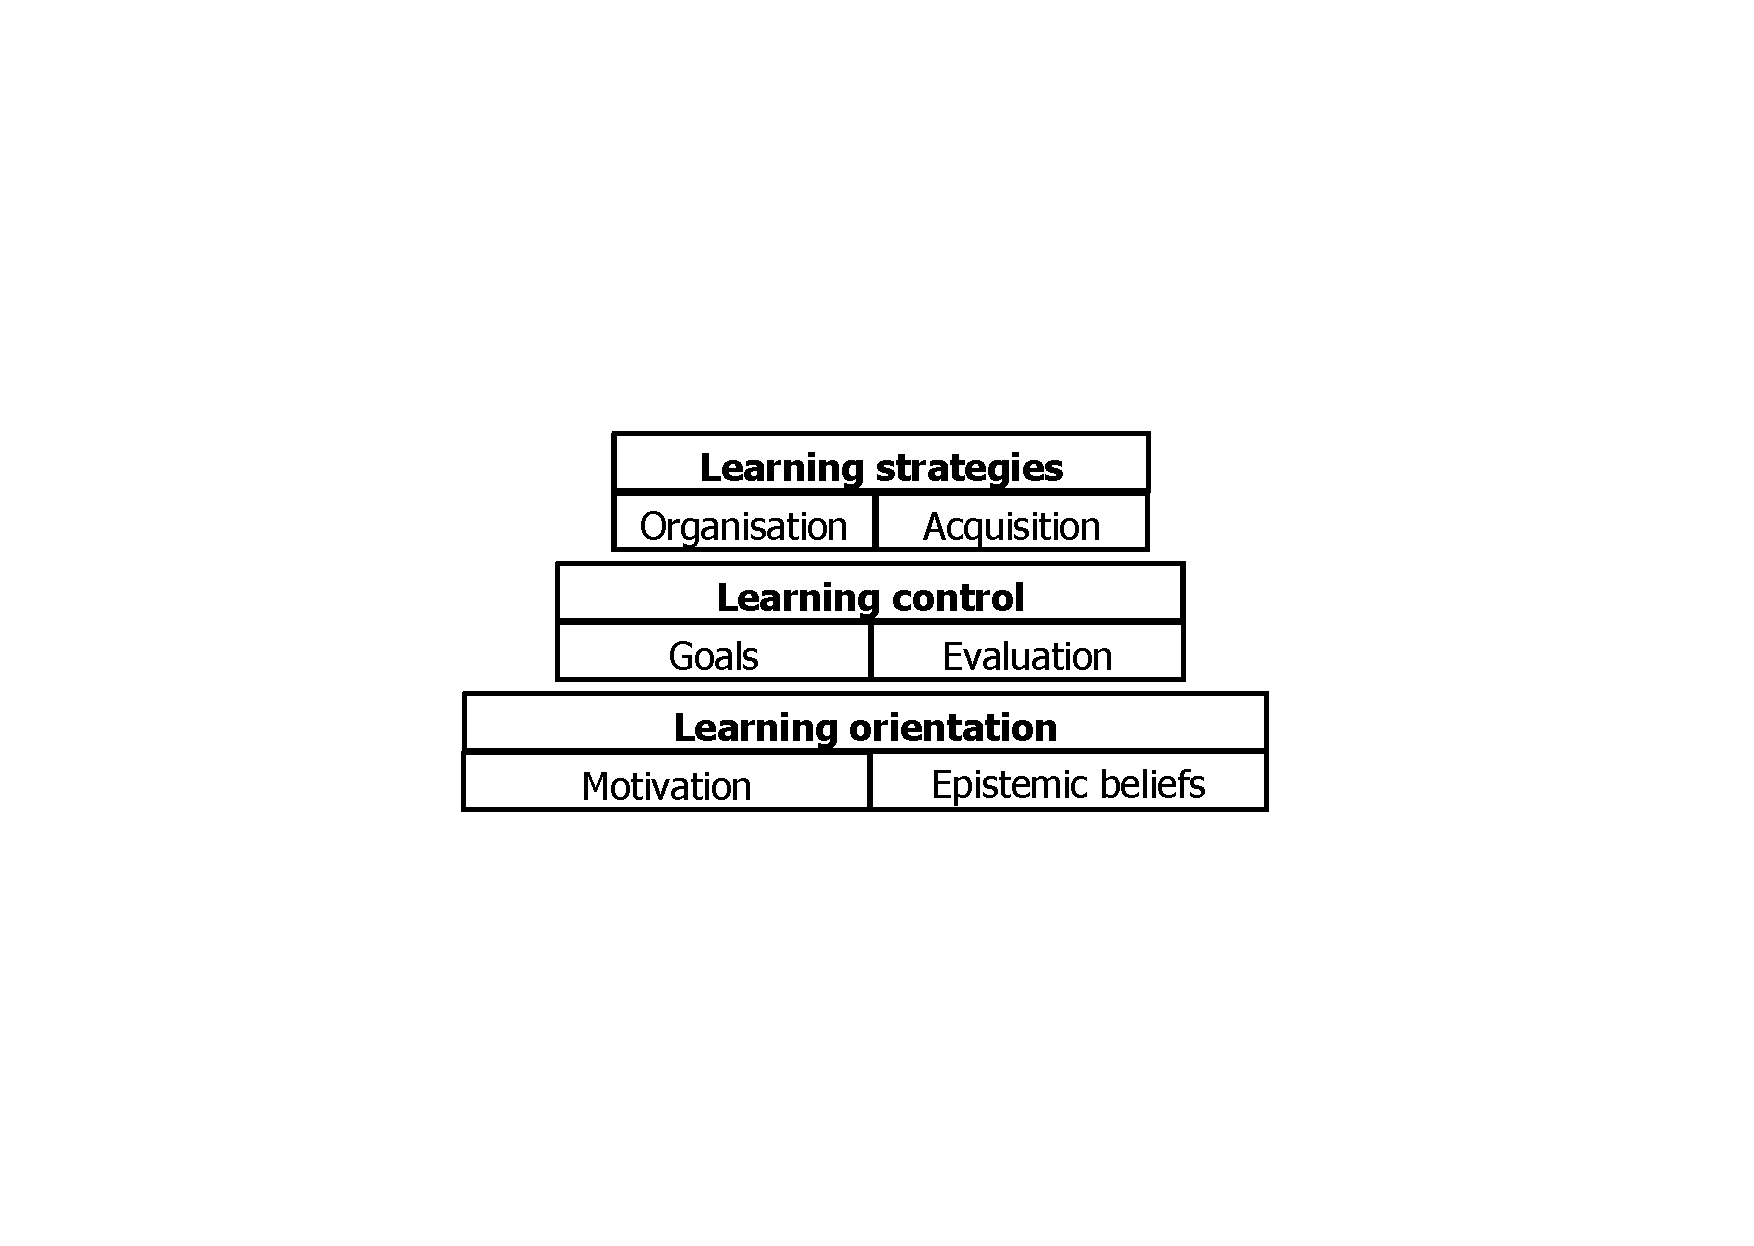
\includegraphics[width=0.5\textwidth,height=8cm]{RR2008CSRImage.pdf}
    \caption{Levels and central constructs of learning competency.}
  \end{center}
\end{figure}

\begin{flushleft}
\textbf{Research Highlights 2007/2008}
\end{flushleft}

We began with employee surveys assessing the interplay of meta-cognitive and motivational variables, and the influence of organizational variables (e.g., T\&D climate, learning opportunities at work) on learning competency. Results indicated that older workers showed learning competency decreases from declines in memory self-efficacy (MSE) rather than as a function of biological age. As such declines are particularly likely in organizations that offer few learning opportunities, and that fail to encourage continuous T\&D participation, older workers are more likely than their younger colleagues to experience MSE decline; it may thus be seen as a secondary age effect. We follow up on these findings in laboratory research investigating the interplay of age, MSE, and task difficulty in cognitive resource allocation to self-regulated learning tasks in an e-learning environment. Intervention studies follow naturally from this approach, and thus they form a third focus of our research. We have started designing "learning competency workshops" that seek to enhance learning performance by training goal-setting and monitoring skills.


\subsubsection{Age-Related Changes in Work Motivation }


\begin{flushleft}
\textbf{Research Program}
\end{flushleft}


Given decreasing numbers of young workforce entrants, the successful retention of older workers is of high importance for many organizations; this requires a profound understanding of older workers' motivation. While aging, more often than not, is perceived to involve inevitable decline in motivation, we posit that age-related changes in work motivation might be conceptualized as outcomes of active regulation. Rather than passively responding to personal (e.g., capability declines) and environmental (e.g., altered work demands) changes, older workers actively adapt to these changes. As a result, work motivation becomes more task-specific; the influence of work context on motivation changes both quantitatively and qualitatively and leads to developing an individual motivational profile (Stamov Ro�nagel, in press).

\paragraph{}
In co-operation with various companies, we develop within this framework tools for motivation diagnostics and interventions. We seek to identify specific areas of age-related increases and decreases. Beyond academic interest, conceptualizing age-related changes in motivation as an outcome of active regulation might provide human resource professionals with more opportunities for motivation interventions. For instance, giving older workers higher degrees of job control might help fulfill their needs for job customization, and may enable them to allocate effort in line with their motivational profile. In a similar vein, discussing and "teaching" motivational regulation strategies might help equip older workers with skills to successfully cope with age-related capability changes and changing job demands. Finally, research into motivation profiles might increase the effectiveness and efficiency of motivational interventions, and might be fruitful for building (age-diverse) teams.

\paragraph{}
\begin{flushleft}
\textbf{Research Highlights 2007/2008}
\end{flushleft}

In a recently completed survey, we asked 312 workers (ages 18-65) from a company to rate how motivated they were for their work in general and for tasks emphasizing collaboration with colleagues, demonstration of one's knowledge and skills, learning new skills or knowledge, leading others, working autonomously, and passing to colleagues one's knowledge and experience, respectively. Moreover, to assess needs-supplies fit, participants indicated whether they felt they were given sufficient opportunities to work on each of these task types. We found that the motivation patterns as defined by the six aforementioned types of tasks differed as a function of age. Most importantly, older workers showed higher levels of motivation than their younger colleagues on the "people tasks" involving passing on knowledge and experience and leading others. Independent of age, the overall level of motivation was higher for participants who reported good fit, that is, older workers who reported high needs-supplies fit rated their overall motivation on a comparable level than their younger colleagues. Also, high levels of fit were associated with positive affect at work, indicating that task-specific motivation regulation might be a useful strategy of affect regulation.


\subsubsection{Older Workers' Cognitive Resources for Innovation Behavior }



Most recently, we have embarked on innovation behavior research, which will be funded by a Volkswagen Foundation grant until 2011. Similar to the situation with workplace learning and motivation research, older workers have been somewhat neglected in this field. Although the demand for innovation increases in the wake of technological change and globalization, and although a growing number of older workers will be involved in innovation-related work roles, little research has dealt with the question how age might affect innovation behavior.

\paragraph{} 
Our research focuses on the motivation-cognition interface. We assume that while aging might objectively affect older workers' cognitive innovation resources, workers will strive to compensate for declining resources availability if such compensation is supported by the organization. Routinization, a facet of expertise, is a resource of particular interest in this regard. It frees up cognitive capacity that in an innovation-supporting environment might be directed towards recognizing innovation potentials and developing implementation strategies. In a less supportive environment, however, routinization may be married with unproductive routine. Like for our workplace learning and motivation research, we develop a combination of quantitative survey and experimental methods to investigate the role of personal cognitive resources.


\subsubsection{Collaborators }

%\input{326}
\begin{itemize}
\item University of Heidelberg; \\Sonja Bausch.
\item University of Dortmund;\\ Michael Falkenstein.
\item University of Oldenburg;\\ Prof. Dr. Barbara Moschner.
\item University of Passau;\\ Prof. Dr. Franz Lehner.
\item Portland State University;\\ Prof. Dr. Pamela Tierney.
\item Bremen-Nord Hospital.
\item Deutsche Bank.
\item EnBW.
\item HeidelbergCement.
\item OTTO Group.
\end{itemize}


\subsubsection{Other Professional Activities }


\textit{Ad-hoc reviews:}
Applied Psychology: An International Review, European Journal of Personality, Journal of Behavioural Sciences, Zeitschrift f�r Personalpsychologie, Zeitschrift f�r Sozialpsychologie. \\

\textit{Boards 2007/2008}

\begin{itemize}
\item EU Commission. Member of the Board of Judges, \textit{European Union eInclusion Awards.}
\item Federal Institute of Occupational Health and Safety (BAuA), Advisory Board Member of the PFIFF project.
\end{itemize}

\subsubsection{Publications }

\begin{itemize}

\item Stamov Ro�nagel, C. (in press). Motivationsregulation �lterer Besch�ftigter. In K. Brauer \& G. Korge, editor, \textit{Perspektive 50plus? Theoretische und Praktische Ans�tze zur regionalen Arbeitsmarktf�rderung �lterer.} Wiesbaden: Verlag f�r Sozialwissenschaften. 

\item Stamov Ro�nagel, C. (in press). Arbeitsmotivation �ber die Lebensspanne: Aktive Regulation statt passiven Abbaus. In J. Kocka, M. Kohli, \& W. Streeck (Hrsg.), \textit{Altern, Familie, Zivilgesellschaft und Politik.} Stuttgart: Wissenschaftliche Verlagsgesellschaft.

\item Stamov Ro�nagel, C. (in press). Was H�nschen nicht lernt...? Folgen der Altersselektion bei Weiterbildungskonzepten. In K. Brauer \& W. Clemens (Hrsg.).\textit{ Zu Alt? Zur Theorie des Ageism und zur Empirie der Altersdiskriminierung auf Arbeitsm�rkten}. Wiesbaden: Verlag f�r Sozialwissenschaften.

\item Gotoh, F., Kikuchi, T., \& Stamov Ro�nagel, C. (2008). Emotional Interference in Enumeration: A Working Memory Perspective. \textit{Psychology Science Quarterly}, 50 (4), 526-537.

\item Stamov Ro�nagel, C. (2008). Motivationsregulation �lterer Besch�ftigter. In K. Brauer \& G. Korge (Eds.), \textit{Perspektive 50plus? Theoretische und Praktische Ans�tze zur regionalen Arbeitsmarktf�rderung �lterer} (p. 71-86). Wiesbaden: Verlag f�r Sozialwissenschaften.

\item Stamov Ro�nagel, C. (2008). \textit{Mythos "Alter Mitarbeiter": Lernkompetenz jenseits der 40}? Weinheim: Beltz PVU.

\item Stamov Ro�nagel, C., Picard, M.A., \& Voelpel, S. (2008). Weiterbildung jenseits der 40. \textit{Personal}, 36-38.

\item Lehner, F. \& Ro�nagel, C. (2008). iVideo - An Easy-to-use Authoring Tool for Interactive E-Learning Videos. In Luca, J. \& Weippl, E.R. editors, \textit{Proceedings of ED-MEDIA 2008 - World Conference on Educational Multimedia, Hypermedia \& Telecommunications} (5373 - 5378). Chesapeake, VA: AACE. 

\item Staudinger, U. M., Ro�nagel, C., \& V�lpel, S. (2008). Strategische Personalentwicklung und demographischer Wandel - eine interdisziplin�re Perspektive. In K. Schwuchow \& J. Gutmann, J., editors, \textit{Jahrbuch Personalentwicklung 2008 - Ausbildung, Weiterbildung, Management Development} (295-304). M�nchen: Luchterhand.

\item Ro�nagel, C. \& Schulz, M. (2007). Besch�ftigungsf�higkeit erfahrener Mitarbeiter. sichern - welche Rolle spielt die betriebliche Weiterbildung Ergebnisse einer Befragung von Unternehmen in Ostwestfalen-Lippe. G�tersloh: Bertelsmann.

\item Ro�nagel, C. \& Voelpel, S. (2007). Qualifizierung �lterer Mitarbeiter: Keine Einheitsweiterbildung. \textit{Persorama}, 35, 24-29.

\end{itemize}


\subsection{A Perspective from Business Administration on the Aging 	Workforce}



\subsubsection{WISE Research Group in Business Administration}

\paragraph{Research Team}

Sven Voelpel (Professor of Business Administration), Torsten Biemann (Postdoctoral Fellow; since 09/2007), Robert Eckhoff (Doctoral Fellow; since 10/2007), Polina Isichenko (Doctoral Fellow), Eric Kearney (Postdoctoral Fellow; since 10/2007), J�rg Korff (Doctoral Fellow; since 08/2007), Claudia Licklederer (Doctoral Fellow; since 07/2008), Daniela Noethen (Doctoral Fellow; since 04/2007), Anne Sauer (Doctoral Fellow; since 10/2008), Stefan Schaffer (Doctoral Fellow; since 11/2007), Katharina Speckmann (Doctoral Fellow; since 05/2008), Eden Tekie (Doctoral Fellow), Chunli Zhao (Doctoral Fellow).

%\newpage

\paragraph{}
Organizations must respond to a number of challenges brought about by major economic, technological, and demographic changes as well as heightened competition. There are many ways in which organizations can meet these challenges and gain competitive advantages. Generally, we examine the topics of wisdom, innovation, strategy, and energy in organizations. We investigate how the ongoing demographic changes and the rising average age in the workforce effect organizational outcomes in these domains (Voelpel, Leibold, \& Fr�chtenicht, 2007). Figure 16 provides an overview of these research efforts.

\paragraph{}
As a specific example of our research, we study how organizational teams should be composed to ensure high levels of performance and low levels of dysfunctional processes. In this regard, many authors view team heterogeneity (diversity) as a potential for increased creativity and innovation. Most importantly, we study under what conditions and through what processes age diversity can enhance team performance (Kearney, Voelpel, \& Gebert, 2008). 

\paragraph{}
\textit{Central Reference}

\paragraph{}
Voelpel, S., Leibold, M., \& Fr�chtenicht, J.-D. (2007). \textit{Herausforderung 50 plus: Konzepte zum Management der Aging Workforce: Die Antwort auf das demographische Dilemma.} Erlangen - New York: Publicis-Wiley (Vorwort von Heinrich von Pierer; Vorwort von Klaus Jacobs).

\paragraph{The WISE research domains are depicted in the following figure: }

\begin{figure}[htb]
  \begin{center}
    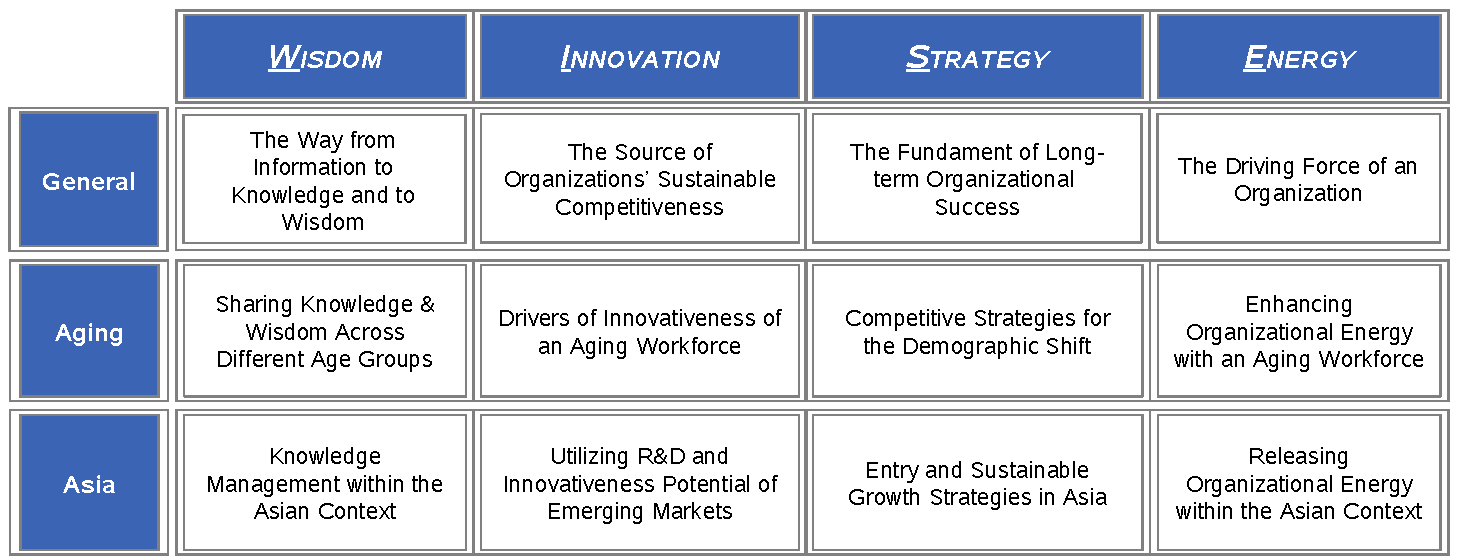
\includegraphics[width=0.5\textwidth,height=5cm]{profSvenVoelpel-fig1}
    \caption{Wise Research Domains }
    \label{fig1:profSvenVoelpel}
  \end{center}
\end{figure}

%\begin{flushleft}
%    \begin{tabular}{ | l | p{3cm} | p{3cm} | p{3cm} | p{3cm} |}
%    \hline
%        & \href{http://www.wiseresearch.org/index.php?do=wisdom}{WISDOM}  
%        & \href{http://www.wiseresearch.org/index.php?do=innov}{INNOVATION} 
%        & \href{http://www.wiseresearch.org/index.php?do=strategy}{STRATEGY} 
%        & \href{http://www.wiseresearch.org/index.php?do=energy}{ENERGY} \\ \hline
%    
%    GENERAL 
%    & \href{http://www.wiseresearch.org/index.php?do=wisdom}{The Way from Information to Knowledge and to Wisdom.}
%    & \href{http://www.wiseresearch.org/index.php?do=innov}{The Source of Organizations' Sustainable Competitiveness.}
%    & \href{http://www.wiseresearch.org/index.php?do=strategy}{The Foundation of Long-term Organizational Thrust.}
%    & \href{http://www.wiseresearch.org/index.php?do=energy}{The Driving Force of an Organization.} \\ \hline
    
%    AGING 
%    & \href{http://www.wiseresearch.org/index.php?do=energy}{Sharing Knowledge \& Wisdom Across Different Age Groups.} 
%    & \href{http://www.wiseresearch.org/index.php?do=innov&div=aging}{Drivers of Innovativeness of Aging Workforce.}
%    & \href{http://www.wiseresearch.org/index.php?do=strategy&div=aging}{Competitive Strategies for the Demographic Shift.}
%    & \href{http://www.wiseresearch.org/index.php?do=energy&div=aging}{Enhancing Organizational Energy with an Aging Workforce.} \\ \hline
    
%    ASIA 
%    & \href{http://www.wiseresearch.org/index.php?do=wisdom&div=asia}{Knowledge Management within the Asian Context. }
%    & \href{http://www.wiseresearch.org/index.php?do=innov&div=asia}{Utilizing R\&D and Innovativeness Potential of Emerging Markets.}
%    & \href{http://www.wiseresearch.org/index.php?do=strategy&div=asia}{Entry and Sustainable Growth Strategies in Asia. }
%    & RReleasing Organizational Energy within the Asian Context. \\ \hline
    
%    \end{tabular}

%\end{flushleft}

\subsubsection{WISE Demographic Network (WDN)}

\paragraph{Research Program}
On March 28$^{th}$ 2007, we founded the WISE Demographic Network (WDN) at the World Business Dialogue in Cologne. In times of demographic change, it is our objective to create strategic cooperation that aims to provide competitive advantages by enhancing innovation and productivity. Based on cooperation between academic research and organizations, practically applicable recommendations are formulated and tailored for individual organizations. Furthermore, it is intended that best practices and knowledge be exchanged. Another objective of the WISE Group is profiling an interdisciplinary research area. We have eight partner companies in the WDN:

\begin{itemize}

\item Daimler AG
\item Deutsche Bahn AG
\item Deutsche Bank AG
\item EnBW - Energie Baden-W�rttemberg AG
\item Lonza Ltd.
\item Mars GmbH
\item Otto GmbH \& Co. KG
\item Volkswagen AG

\end{itemize}

\paragraph{Research Highlights 2007/2008}
The WISE Demographic Network has conducted a qualitative analysis of its members' current status in terms of their demographic fitness. On the basis of a tailored focus group guideline, we identified the major fields of action of each member company. The analysis and comparison of the data of all member companies provided a solid basis for deriving various potential research strands. We have focused on three major issues that are of interest to all organizations: 

(1) Mechanisms, requirements, and obstacles of workplace learning;


(2) Employee organization amenable to achieving successful knowledge transfer (Teams)  and


(3) Age-differentiated application of HR practices (Talent Management). 

Three full-day WDN member conferences arranged in Bremen (October 07), Frankfurt (April 08), and Karlsruhe (October 08) helped to advance customized study efforts as well as best practice exchange.

\begin{figure}[htb]
  \begin{center}
    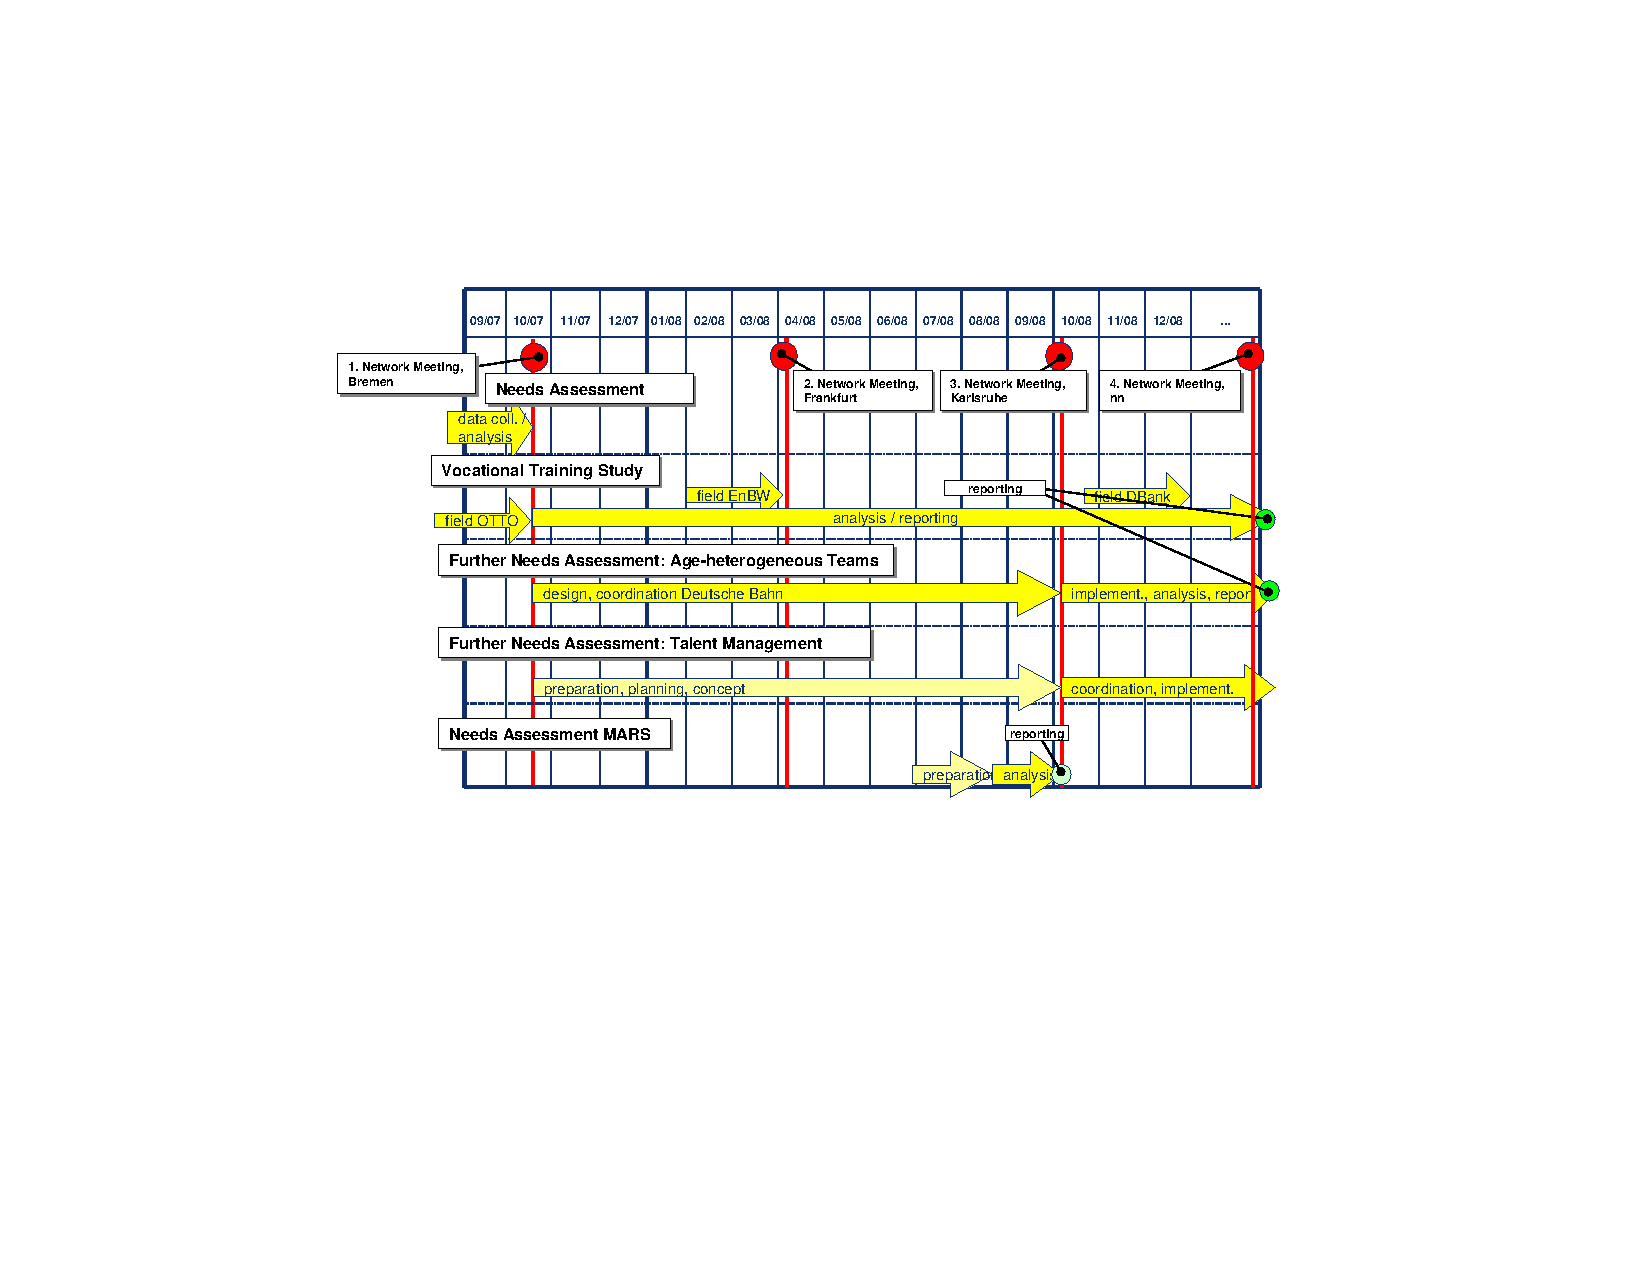
\includegraphics[width=0.5\textwidth,height=6.5cm]{Figure17_SV.pdf}
    \caption{WDN Activities.}
  \end{center}
\end{figure}


\subsubsection{Enhancing Aging Talents - Adjustment of Human Resource Management}

\paragraph{}

\begin{flushleft}
\textbf{Research Program}
\end{flushleft}


Research from strategic human resource management has provided sound evidence for the positive association between HR practices and organizationally valued performance (HRM-P). No theoretical framework has yet been provided, however, that is able to explain this relation.

\paragraph{}

\begin{flushleft}
\textbf{Research Highlights 2007/2008}
\end{flushleft}

In this project, an integrated HRM-P was developed that includes mediating variables that have been found empirically to be associated with organizational performance; these variables include (1) work motivation, (2) job satisfaction, and (3) organizational commitment (see Figure 18). The moderating role of employees' age for the mediated association was analyzed. The model aims to provide organizations with a basis on which to adjust their management tools in order to meet personnel challenges that have evolved due to demographic changes; this will permit employers and other relevant actors to preserve competitiveness.

\begin{figure}[htb]
  \begin{center}
    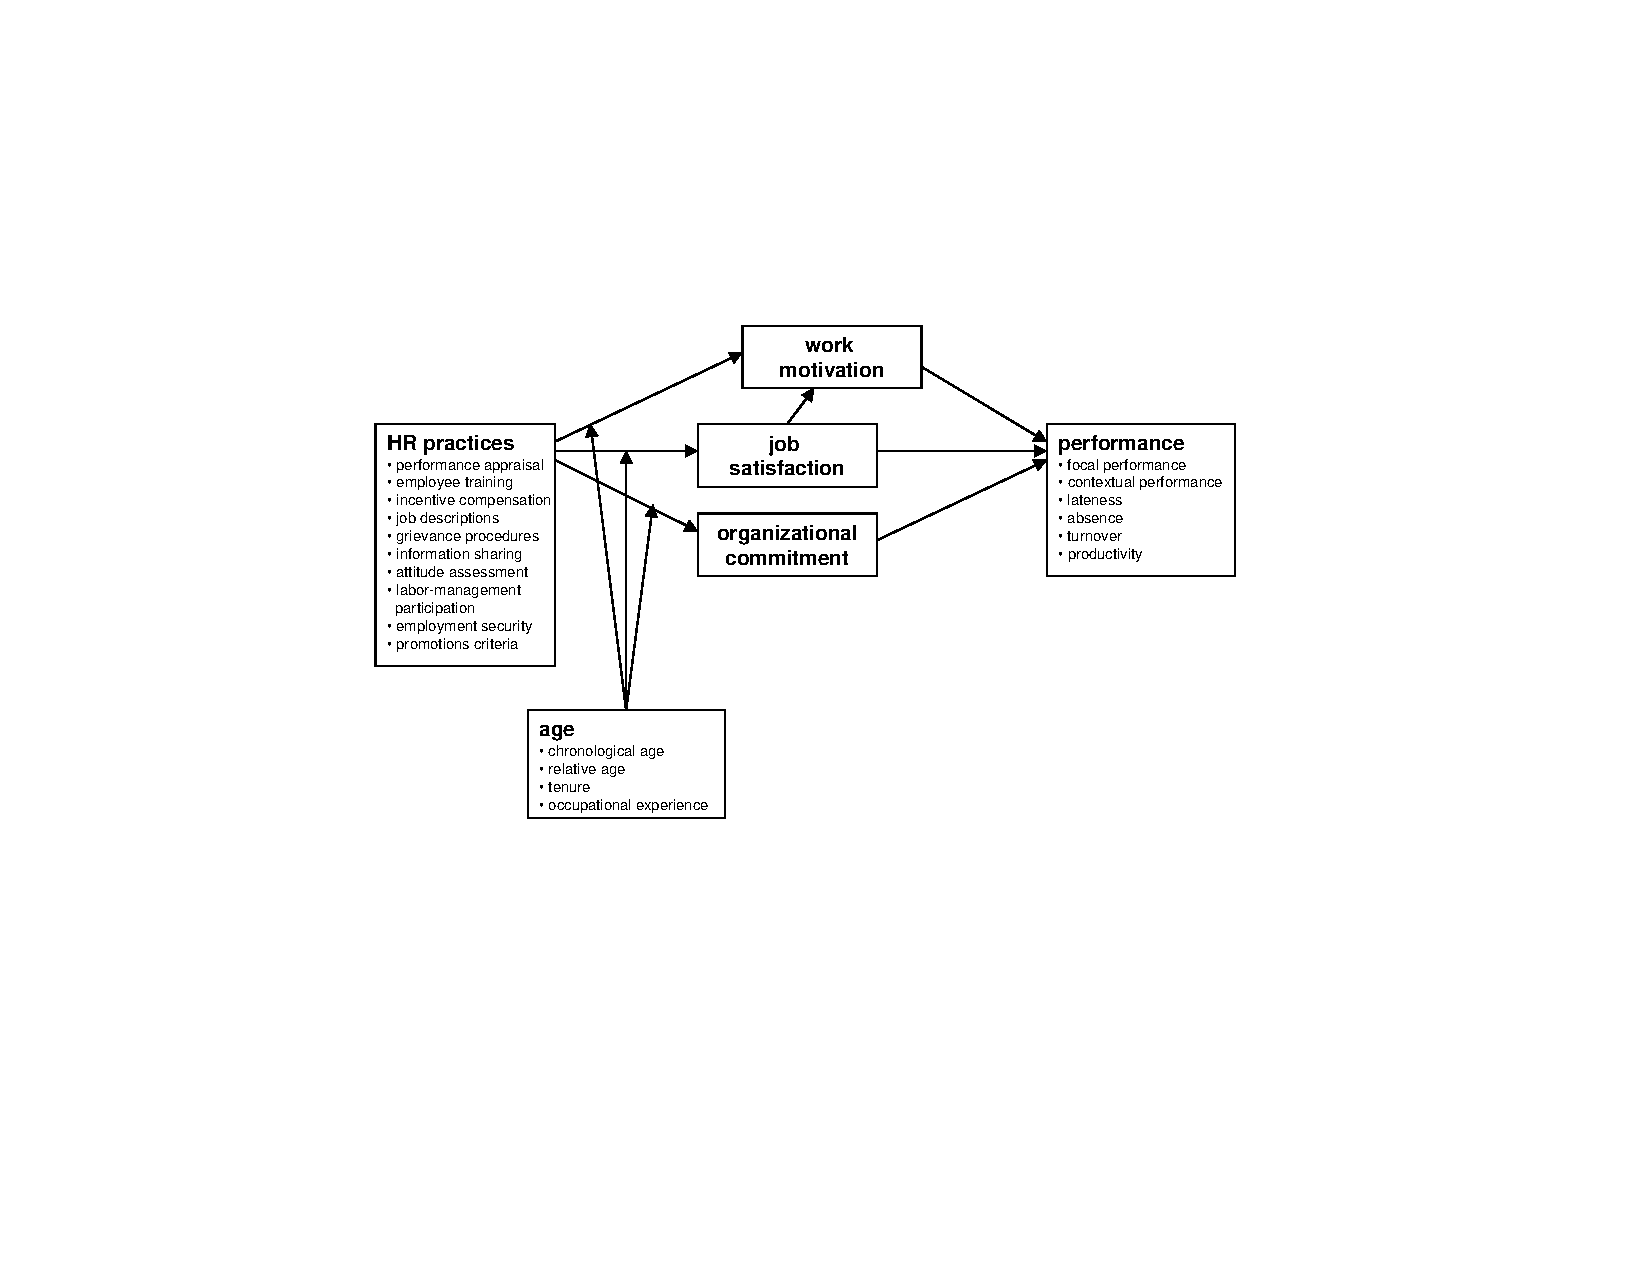
\includegraphics[width=0.5\textwidth,height=6.5cm]{Figure18_SV.pdf}
    \caption{Basic Research Model for the moderated and mediated relationship between HR practices and performance.}
    \label{Figure18_SV}
  \end{center}
\end{figure}

\paragraph{}
The model delineated above is primarily intended to be applied in the context of actual work settings. Taking this into account, we plan to gather empirical data by conducting surveys within various organizations. The project is currently acquiring organizations that are interested in participating in the empirical study.

\subsubsection{Knowledge Transfer: Demopass}

Analysing data from the interdisciplinary demopass-project (see 2.1), we are looking at influences on knowledge transfer within teams with a special focus on knowledge transfer between older (i.e. over 45 yrs.) and younger employees (i.e. under 30 yrs.). Moreover, we are investigating the connection between these types of knowledge transfer and performance. In terms of influences on knowledge transfer, we found a strong age effect with older employees engaging more in sharing knowledge with other team members while younger employees seek more knowledge from team members. In addition, employees in teams that have a lower average age in comparison to other teams seek more knowledge from team members. Furthermore, we found that extrinsic or intrinsic benefits motivate knowledge transfer within teams; while intrinsic benefits significantly influence individual knowledge sharing, extrinsic benefits motivate knowledge seeking. Finally, we found that high individual job autonomy encourages knowledge sharing while working in a team with high average job autonomy (compared to other teams) encourages individual knowledge seeking. Results on the connection between knowledge transfer and performance are forthcoming.

\subsubsection{Intergenerational Knowledge Transfer to Prevent Knowledge Loss in Organizations}

\paragraph{}

\begin{flushleft}
\textbf{Research Program}
\end{flushleft}

In the last decade, a knowledge-based perspective of the firm has emerged in strategic management literature. Knowledge is now seen as a resource that enhances productivity and conveys a competitive advantage for organizations. If older employees, with decades of experience, leave an organization, they take with them critical knowledge that they alone may possess, and whose loss leads to high costs for the organization. Although it has always been the case that employees retire and new employees are hired, this is especially problematic today because:

\begin{itemize}

\item Knowledge-intensive domains have become increasingly more specialized, complex and interdisciplinary;
\item Demographic changes, particularly waves of retiring baby boomers, have created new challenges; and
\item  Employees are now changing companies more often.

\end{itemize}

\paragraph{}

\begin{flushleft}
\textbf{Research Highlights 2007/2008}
\end{flushleft}

Several strategies have been proposed to prevent the costly loss of knowledge: they often involve, but are not limited to, HR processes, IT-tools, knowledge recovery initiatives, and knowledge transfer.
This project is focusing on the latter, proposing a coherent model of antecedents of knowledge transfer, as well as trying to establish a link between knowledge transfer between employees and the reduction of the threat of knowledge loss for an organization (see Figure 19). The objectives of this project can be summarized in three broad research questions:
\begin{enumerate}
	\item What are the main antecedents of knowledge sharing and knowledge seeking?
	\item Where does age play a role?
	\item Does knowledge transfer reduce the threat of knowledge loss?
\end{enumerate}

The project is currently in the phase of analyzing the empirical data. In addition, we intend to acquire additional organizations as collaboration partners.

%\begin{figure}[htb]
%  \begin{center}
%    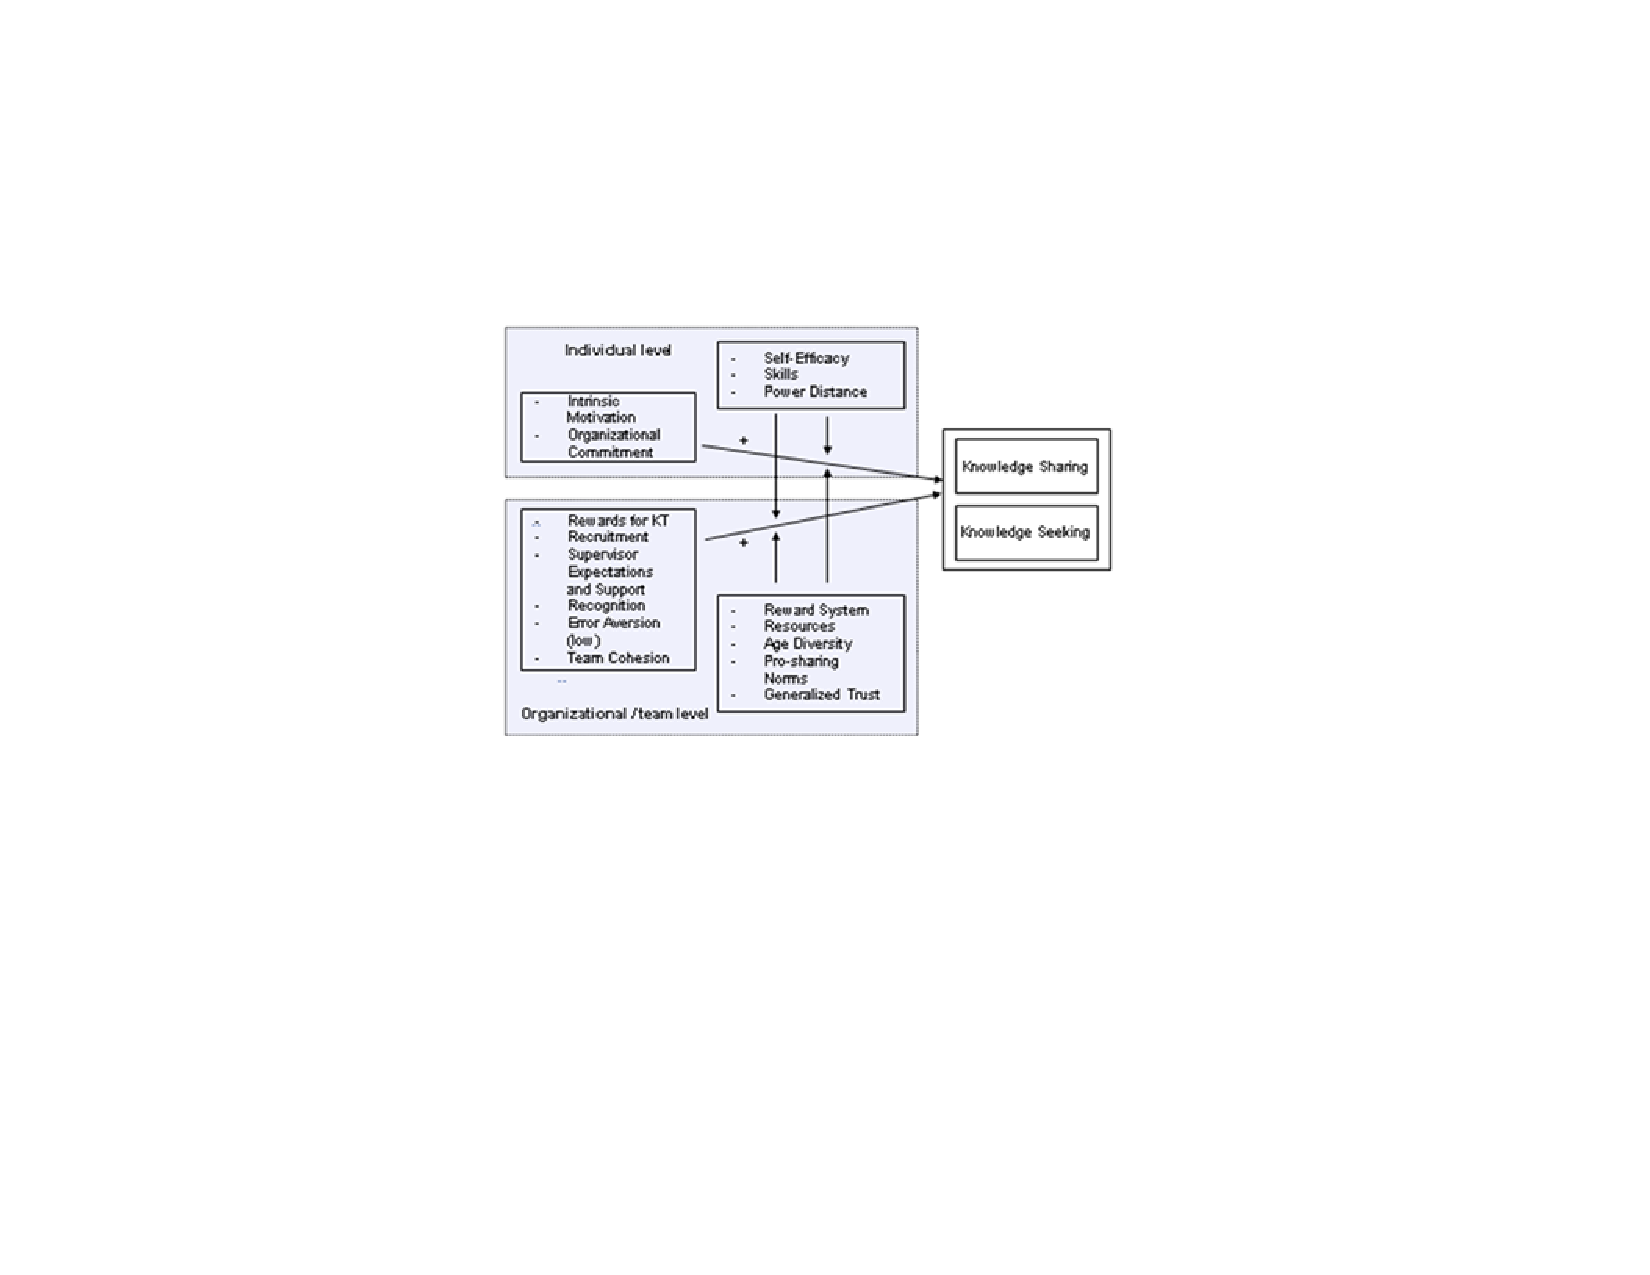
\includegraphics[width=0.5\textwidth,height=5cm]{Figure19_SV.pdf}
%    \caption{Basic research model on the antecedents of knowledge seeking and sharing.}
%  \end{center}
%\end{figure}

\paragraph{}
Within this broader framework of individual knowledge sharing in organizations, another focus is on knowledge exchange between different hierarchical levels, an aspect that very often also involves a difference in age. The objective of this empirical study is to investigate the decisive factors that influence employees' engagement in knowledge sharing with their supervisors.

\subsubsection{The Effects of the Aging Workforce on the Innovation Process: A Large-Scale Study of Technology Intensive Companies}

\begin{flushleft}
\textbf{Research Program}
\end{flushleft}

How will the aging of the workforce affect the innovativeness of organizations? The foundation of the innovation is ideas, and it is people who develop, carry, react to, and modify ideas. It is therefore important to recognize that innovation is based on individual and group performance efforts. As a result of the dramatic increase in the number of older employees in the workforces of developed industrial countries, the necessity to create innovation is more often than ever entrusted to aging employees. From this perspective, it is important to understand how this demographic trend changes individual and group behavior as it relates to innovation. 

\paragraph{}
Research has only recently begun to consider the relationship between the aging of workforces and the state of innovation processes. Unfortunately, this research has produced equivocal outcomes. We suggest that this is caused by: (a) a failure of the studies to include intervening processes that explain differences in innovative work behaviors across age cohorts; (b) a lack of distinction between radical and incremental idea-generation behaviors; (c) a paucity of empirical research on the relationship between aging and innovation in organizational settings; and (d) a neglect of the effects of increasing age diversity on group innovativeness. 

\paragraph{}
The goal of this research project is to overcome these knowledge gaps by developing a framework that explains the impacts of an aging workforce on innovation processes in organizational settings. This framework is meant to advance current knowledge in four important ways. First, it will connect aging to the behavioral activities involved in the innovation process through those factors that facilitate innovation. Innovative behavior across three behavioral activities will be analyzed: idea generation, innovation promotion, and implementation. Second, the framework will explore and explain the differences in idea generation patterns, innovation promotion, and implementation work behaviors across age cohorts. Understanding these differences will help us to draw possible conclusions about the implications of the aging of the workforce for organizational innovativeness. Third, it will explore and explain how innovation processes in workgroups are affected by an increase in those workgroups' age diversity. Finally, the framework will describe measures that enable organizations to intervene effectively into the relationship between aging and group innovation. Specifically, recommendations are expected to provide guidance for organizations on how to understand and benefit from innovative work behavior differences between younger and older-age cohorts across activity levels of the innovation process. They will also help companies integrate diverse innovative behaviors of age-dissimilar cohorts.

\paragraph{}
This project will collaborate with its industrial partner in order to access in-depth insights through interviews and surveys conducted in R\&D and technical teams of the company. The R\&D and innovation-related working groups of the industrial partner will serve as the units of analysis for quantitative and qualitative research.

\paragraph{}
Our study will employ a multi-method approach with a mix of quantitative and qualitative methods to generate and test our hypotheses. A concurrent triangulation strategy of the multi-method approach will be applied in order to confirm and cross-validate findings within a single study. The project will comprise a preparation phase, a study of mediators and moderators of the effect of age on the innovation behavior, a study of innovative behavior at individual and group levels, a comparative analysis, and a symposium.

\paragraph{}
We expect this project to generate a number of insights into this emerging and vibrant research topic, and to produce recommendations that will help organizations to improve the innovativeness of teams.

\subsubsection{Collaborations}

\begin{itemize} 
\item Massachusetts Institute of Technology, AgeLab, Prof. Dr. David DeLong 
\item Intellectual Capital Institute of Ireland, David O'Donnell 
\item Harvard Business School, Prof. Dorothy Leonard 
\item Babson College, Prof. Thomas H. Davenport 
\item ETH Zurich, Prof. Dr. Georg Von Krogh 
\item University of Stellenbosch, Prof. Marius Leibold 
\item Hitotsbashi University, Prof. Ikujiro Nonaka 
\item Wharton, Prof. Dr. Martine Haas 
\item Open University, Dr. J.C. Spender 
\item University of St. Gallen, Prof. Heike Bruch 
\item Erasmus University Rotterdam, Prof. Daan van Knippenberg 
\item Autonomous Universidad Madrid, Prof. Ramon Rico 
\item University of Groningen, Prof. Gerben van der Wegt 
\item University of Amsterdam, Prof. Dr. Astrid Homan 
\item Peking University, Prof. Dr. Max von Zedtwitz Gerben van der Wegt
\item Massachusetts Institute of Technology, Prof. Dr. Alan MacCormack 
\item Harvard University, Prof. Michael Beer 
\item University of California, Los Angeles, Prof. Barbara S. Lawrence 

\end{itemize}

\subsubsection{Publications}

\begin{itemize}
\item Voelpel, S., \& Kearney, E. (2008). Trust within organizations - Benefiting from demographic changes by fostering intra-organizational trust. \textit{Forum on Public Policy: Journal of the Oxford Roundtable}, 4(1): 1-17.

\item Kearney, E., Voelpel, S. C., \& Gebert, D. (2008). Examining the interaction of demographic diversity and personality - The role of need for cognition. \textit{Academy of Management Best Paper Proceedings}, 1-6. 
\item Voelpel, S., Eckhoff, R., \& F�rster, J. (2008). David against Goliath? Group size and bystander effects in virtual knowledge sharing. \textit{Human Relations}, 61(2): 273-297. 

\item Streb, C., Voelpel, S., \& Leibold, M. (2008). Managing the aging workforce: Status quo and implications for the advancement of theory and practice. \textit{European Management Journal}, 26(1): 1-10.

\item Han, Z., \& Voelpel, S. (2007). Knowledge Sharing in China: Reflections about Siemens' Experiences with ShareNet. \textit{Journal of Asian Business}, 23(1): 123-143.

\item Voelpel, S., \& Koch, J. (2008). Erfahrene Talente Bringen Weitblick. Fachteil: Demographischer Wandel. \textit{Personalwirtschaft}, 35(10): 44-46.

\item Voelpel, S., \& Koch, J. (2008). Zeitsammler und Talentj�ger. Fachteil: Demographischer Wandel in KMU. \textit{Personalwirtschaft}, 35(9): 46-49.

\item Voelpel, S., \& Koch, J. (2008). Wissen ist Marktstellung. Fachteil: Demographischer Wandel in KMU. \textit{Personalwirtschaft}, 35(8): 44-46.

\item Voelpel, S., \& Koch, J. (2008). Die passende Dosis finden. Fachteil: Demographischer Wandel in KMU. \textit{Personalwirtschaft}, 35(7): 46-48.

\item Voelpel, S., Koch, J. \& Afting, M. (2008). Wir sind DB. Gesichter, Stars und Hidden Champions: Das Talent Management der Deutschen Bahn wird als Kulturmanagement verstanden. \textit{Personal}, 60(7): 62-64.

\item Voelpel, S., \& Koch, J. (2008). Der Blick auf die St�rken. Fachteil: Demographischer Wandel. \textit{Personalwirtschaft}, 35(6): 44-46.

\item Voelpel, S., Koch, J., \& Korff, J. (2008). Die Gro�en im auf dem Weg zur demografischen Fitness. \textit{Personalwirtschaft}, 35(4): 44-46.

\item Ro�nagel, C., Picard, A.., \& Voelpel, S. (2008). Lernen jenseits der 40. \textit{Personal}, 60(4): 40-42.

\item Voelpel, S., \& Koch, J. (2008). Die neuen Davids. \textit{Personalwirtschaft}, 35(2): 49-51.

Otto, S., \& Voelpel, S. (2007). Demographischer Wandel in der Wirtschaft: Warum Unternehmen �ltere Arbeitnehmer brauchen. \textit{�kologisches Wirtschaften}, 26(4): 12-13.

\item Voelpel, S. (2007). Der Student als K�nig und Schwerstarbeiter. Eindr�cke von der Lehre an der Universit�t Harvard. \textit{Forschung \& Lehre}, 14(10): 598-600. 

\item Voelpel, S. (2007). Demografischer Wandel - Sage keiner, er sei nicht gewarnt worden. \textit{Personalwirtschaft}, 34(8): 18-22 (Comment by Wolfgang Clement, Chairman of the Adecco Institute). 

\item Rossnagel, C., \& Voelpel, S. (2007). Qualifizierung �lterer Mitarbeiter: Keine Einheitsweiterbildung. \textit{Persorama}, 31(1): 24-29. 

\item Voelpel, S., von Pierer, H., \& Streb, C. (2007). The mobile company: An integrated model for mobilizing to innovate. \textit{Profile}, 13, 59-65.

\item Staudinger, U. M., Ro�nagel, C. \& Voelpel, S. (2007). Personalmanagement und demographischer Wandel - eine interdisziplin�re Perspektive. In K. Schwuchow \& J. Gutmann, editors, \textit{Jahrbuch Personalentwicklung 2008 - Ausbildung, Weiterbildung, Management Development}�( 295-304). Munich/ Unterschlei�heim: Luchterhand.

\item Voelpel, S., Leibold, M., \& Fr�chtenicht, J.-D. (2007). H\textit{erausforderung 50 plus: Konzepte zum Management der Aging Workforce: Die Antwort auf das demographische Dilemma}. Erlangen - New York: Publicis-Wiley (Vorwort von Heinrich von Pierer; Vorwort von Klaus Jacobs). 

\end{itemize}

\subsection{The Socio-Economics of Lifelong Learning and Aging }


\paragraph{}
\begin{flushleft}
\textbf{Research Team}
\end{flushleft}

Klaus Sch�mann (Professor of Sociology), Paula Aleksandrowicz (Doctoral Fellow; until 06/2008), Stefan Baron (Doctoral Fellow; since 04/2007), Anette Fasang (Doctoral Fellow; until 08/2008; now Postdoctoral Fellow, Yale University), Sara-Izabella Geerdes (Doctoral Fellow), Daniel Schelkes (Doctoral Fellow; since 04/2008), Liuben Siarov (Doctoral Fellow BIGSSS; since 09/2008).

\paragraph{}
Socio-economic research on lifelong learning has to address the increasing impact of aging societies. We do this by applying a combination of economic research (e.g. human capital formation and accumulation) and sociological research (e.g. the social processes of inequality). Identifying market failures and understanding incentive structures with the potential to overcome unequal access to lifelong learning is part of our research program. The research group studies transitions over the life course and analyzes the impact of transitions on learning and employment careers. The life course perspective provides the central analytical tool that allows us to study individual trajectories, their institutional embeddedness, and the evolution of societies as a whole. 

\paragraph{}
Our research focuses on processes of social stratification as they are co-determined by learning processes for adults. We model social processes using two-step procedures: (1) we analyze participation in lifelong learning using age, cohort, and education levels as major determinants of participation and; (2) we observe that participation in lifelong learning is an important explanatory factor in processes of labor market mobility. In addition, our research group is carrying out projects with different firms as cooperation partners, focusing particularly on the aging of the workforce, health and safety at the workplace, strategies of lifelong learning, and skill needs assessment. We apply multilevel approaches that combine information from employees and management on the same topic, in a structured way. 

\paragraph{}
In each of these fields we analyze individual behavior as well as the impact of institutions on the life course. We have a particular interest in the link between working and learning as they concern individuals, households, firms and whole country systems. We study transitions throughout the life course that range from labor market entry and reentry after career breaks to gradual retirement; we pay special attention to changes in labor market institutions. These social dynamics are modeled using a transition theory that is based on notions of coupled oscillations (Sch�mann \& O'Connel, 2002) and synchronization techniques. In order to compare the impact of different institutional settings on individual behavior, we apply comparisons of industrial sectors, regions within a country, or US-EU-wide comparisons. Co-financed research projects deal with socioeconomic aspects of lifelong learning and institutional development in two major areas: (1) lifelong learning and the labor market, and (2) aging and the prevention of early retirement. \\


\begin{flushleft}
\textit{Central Reference } \\
\end{flushleft}


Sch�mann, Klaus (2002) "The theory of labour market transitions applied to the transitional labour market of education and training in: Klaus Sch�mann and Philip J. O'Connell (eds.), Education, Training and Employment Dynamics: Transitional Labour Markets in the European Union, Cheltenham, Edward Elgar, pp. 8-38.

\subsubsection{Lifelong Learning and the Labor Market}

\paragraph{}
\begin{flushleft}
\textbf{Research Program}
\end{flushleft}

Research in this area analyzes the link between lifelong learning and the labor market. We analyze sources of market failure, for example multiple factors responsible for underinvestment in lifelong learning. Persistent imbalances in supply and demand for training lead to a lack of participation in further training. Causal analyses of such behavior that seriously consider the evolution of the life course begin by investigating early labor market experiences and their implications for later experiences in the labor market. Analyses typically focus on transition processes like the first integration into the labor market, job to job transitions or further training transitions. 

\begin{figure}[htb]
  \begin{center}
    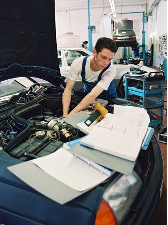
\includegraphics[width=0.5\textwidth,height=10cm]{rr-Kfz-Mechaniker-bei-der-Arbeit.pdf}
  \end{center}
\end{figure}

\paragraph{}
\begin{flushleft}
\textbf{Research Highlights 2007/2008}
\end{flushleft}

Our analyses show that labor market integration of youth follows different trajectories depending on the young person's ethnic background. Young people with a second-generation migration background do not reach comparable entry-level labor market positions. In cases where they do reach jobs with similar types of contracts at entry, they nonetheless tend to have longer job search times (Geerdes et al. forthcoming, based on data from the Socio-economic Panel in Germany). Research also shows that youth and experienced workers do not compete for the same jobs in the labor market. Changes in economic growth have a much stronger impact on youth employment than they do on overall employment; this makes the youth labor market more volatile in general. This leads to better recruitment during favorable business cycles, but decreasing chances at times of slack growth (Hilbert et al., 2007)

\paragraph{}
Early labor market experiences, and particularly educational trajectories, are powerful predictors of participation in lifelong learning. Although the costs of training are due at the moment of participation, returns to training (e.g., increases in productivity or wages, job stability, or promotion) accrue only at some later point in time. Many employees therefore hesitate to take time out from productive work, or reduce working time in the labor market, in order to invest in further training. Risk aversion and budgetary constraints in the form of access to loans for purposes of learning also explain why people are reluctant to participate in training (Dissertation Siarov). In addition, firms might fear the "poaching" of training costs of employees by other firms (although this problem can be addressed by adequate contractual arrangements). Further ways of tackling the barriers to participation in training include: ensuring access to loans, promoting information availability, facilitating certification, the recognition of professional experience, and targeting groups that are the least likely to participate, such as less qualified and older employees. 

\paragraph{}
Research in these fields makes use of longitudinal data (both retrospective and panel), large European surveys, and our own data collected through our Lab III resources such as computer assisted telephone interviews, web-based surveys, or face-to-face interviews. Recent findings show that there are effective policies that can reduce stigmatization of older workers and combat the notion that older workers are less able or less willing to learn. It is therefore not sufficient to increase budgets; it is also necessary to tackle the stigma that perpetuates the view that older people are less interested in learning. Our results, based on an analysis of 20 years of household panel data from Germany, show that younger birth cohorts continue to have higher participation in further training than previous birth cohorts. The generation born between 1950 and 1960 participates on a higher level in further training than earlier cohorts (Sch�mann \& Baron, 2008). 

\paragraph{}
Participation in lifelong learning provides mutual benefits to individuals, firms and society as a whole, and innovative ways to co-finance lifelong learning are particularly promising policy solutions. However, participation in further training remains highly selective with respect to previously obtained levels of education. Our results from a comparative survey (the Eurobarometer, 2005) show that lower qualified individuals are indeed dissatisfied with their lower rates of participation in lifelong learning. This indicates that increasing targeted programs that match specific skill requirements should be successful at raising these low participation rates. 

\paragraph{}
We are also interested in discovering subjective and objective reasons for (non-) participation in lifelong learning (dissertation Baron). More specifically, with data from the interdisciplinary demopass project (see also 2.1) we examined potential influences on individuals' self-confidence in their own training competencies. Following social rational choice theories (e.g. Breen \& Goldthorpe, 1997, Esser, 2001), high self-confidence in one's own competencies is an important precondition for future participation in training. We found that people perceiving a higher training support by their supervisor and better learning climate tend to report a higher self-confidence (Baron \& Sch�mann, in prep.). This is particularly important for lower educated and older employees. It also constitutes new ways to enhance training participation rates of otherwise disadvantaged groups. However, we also identified mismatches between supervisors and associates in the evaluation of teams' training climate. Team members attach less importance to further training than their supervisors, whereas management does not meet employees' training needs.

\begin{figure}[htb]
  \begin{center}
    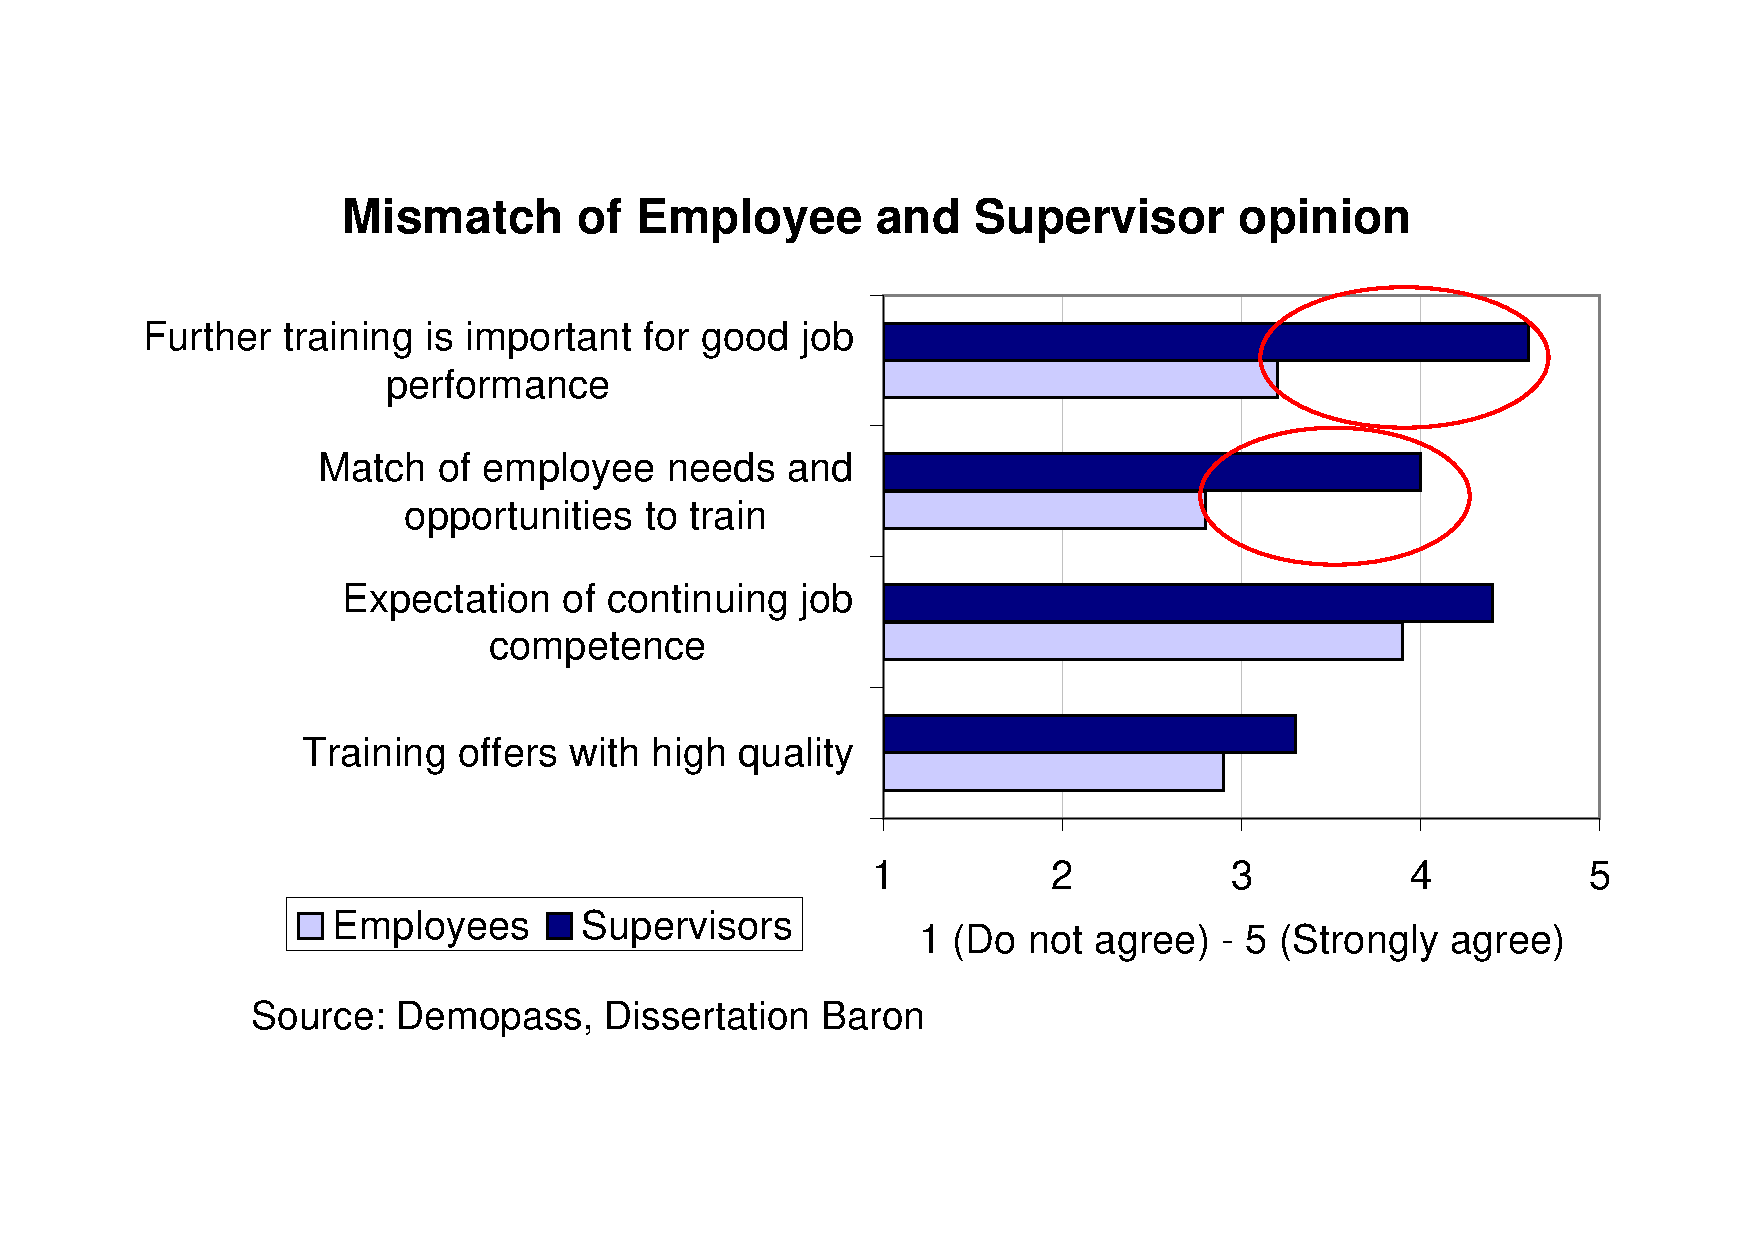
\includegraphics[width=0.5\textwidth,height=6.5cm]{MismatchFirmTrainingClimateChart.pdf}
    \caption{Matches/ Mismatches in firms' training climate. Source: Demopass, Dissertation Baron.}
  \end{center}
\end{figure}

\paragraph{}
Such mismatches can lead to discontent on both sides and as a direct consequence to lower participation rates in training. In sum, our results indicate that training programs should match specific skill requirements as closely as possible. This seems to be a necessary condition to raise the low participation rates of "silver" workers and low training groups in the labor market.

\subsubsection{Aging and the Prevention of Early Retirement}

\paragraph{}

\begin{flushleft}
\textbf{Research Program}
\end{flushleft}

The aging of the working population and the shrinking size of the population of working-age individuals in the near future will create a challenge to all components of welfare states. In order to enable a continuing potential for economic growth in rapidly aging societies, it will be necessary that more "silver workers" continue to work from each birth cohort. At the same time, new ways need to be found to facilitate an extension of working lives for these silver workers. This is the subject of our research interest in the field of productive aging. 

\begin{figure}[htb]
  \begin{center}
    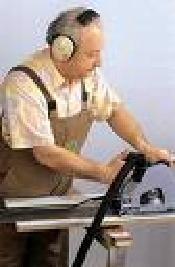
\includegraphics[width=0.4\textwidth,height=8cm]{rrgehorschutz.pdf}
  \end{center}
\end{figure}


\paragraph{}
\begin{flushleft}
\textbf{Research Highlights 2007/2008}
\end{flushleft}

We analyze this topic, for example, with emphasis on how to reverse the trend towards earlier and unequal retirement ages across industrially advanced societies. For this purpose we have compared retirement processes of the 1930-1940 birth cohorts in West Germany and those in the United Kingdom in order to assess how country specific labor market and pension regulations interact in structuring retirement processes. Our results indicate that, for Germany, the standardizing effects of the male breadwinner model occur across all different pathways to old-age pension. This has resulted in comparatively low household inequality at older ages. It is interesting to note that this somehow compensates for high personal inequality between women and men. For the United Kingdom, access to occupational or private pensions by at least one household member aggravates the divide between financially advantaged and less advantaged households (Fasang, 2008). 

\paragraph{}
In addition to labor and pension regulations, we include family biographies in our analyses of productive aging. We compare West Germany and the United Kingdom in order to assess how divorce effects the pension entrance of men and women born between 1930 and 1939. The life courses of these cohorts evolved in a strong male-breadwinner context in both countries, but were subject to different pension regulations (i.e. enforced pension sharing upon divorce in West Germany, and optional pension sharing in the United Kingdom). Pension sharing in Germany leads divorced women to enter old-age pension earlier and divorced men to enter later. In the United Kingdom, where pension sharing was not practiced, we find opposite effects (Fasang \& Sch�mann, 2008). 

\paragraph{}
Working jointly with local enterprises, we assessed the potential of older employees to continue working despite early retirement offers. The results of a company survey comparing early retirees and a similarly aged control group (still working) show that, while at work, employees have a high tendency to accept early retirement, but once in early retirement they soon begin to search for new challenges in the form of work or civic engagement (Aleksandrowicz et al., in press; see also 3.3). 

\paragraph{}
Overall, our work on retirement transitions and health and safety at work (Dissertation Schelkes) gives reason to believe that the prevention of early retirement is a multifaceted transition that requires careful analytical approaches in order to disentangle relevant causalities. The prevention of early retirement, and even the extension of working lives beyond 65, have become more feasible solutions based on sound analytical work. 

\paragraph{}
he recently approved project on "Job Mobility and Developmental Outcomes", co-financed by the Volkswagen Foundation (joint project with Staudinger and Godde; see also 2.2), allows us to assess the impact of cumulative labor market careers on individuals' learning strategies and adaptability at older ages. In a counterfactual design we will contrast matched (medium and low-skill) samples of persons with long labor market careers with meaningful, voluntary job changes, with those who have had few job changes. In a subsequent FMRI study both groups will participate in neurophysiologic tests. The results will give insights on cognitive and personality related adaptability (including learning strategies) of individuals in the two groups, and the interaction of adaptability with underlying neuronal processes. 

\subsubsection{Collaborations}

\begin{itemize}

\item Center for Research on Inequalities and the Life Course (CIQLE), Yale University; Prof. K.U. Mayer.
\item Center on Migration and Development, Princeton University; Prof. Marta Tienda.
\item Institute for Labour Studies (OSA), University of Tilburg; Prof. Ruud Muffels and Prof. Joop Schipers.  
\item Economic and Social Research Institute (ESRI), Dublin; Prof. Philip O'Connell.
\item Social Economic Research Rotterdam (SEOR), University of Rotterdam; Prof. Jaap de Koning. 
\item Institut f�r H�here Studien (IHS), Wien; Prof. Dr. Lorenz Lassnigg. 
\item MATISSE, Centre National de la Recherche Scientifique, Paris I; Prof. Bernard Gazier.
\item Centre for Labour Market Research (CARMA), Aalborg University; Prof. Per Madsen.
\item Research Centre for Education and the Labour Market (ROA), Maastricht University; Prof. Rolf van der Velden. 
\item Institute for Labour Studies (HIVA), Catholic University Leuven - co-ordinator Dr. Tom Vandenberghe.
\item University of North Carolina at Chapel Hill; Prof. Dr. Arne Kalleberg.

\end{itemize}

\subsubsection{Other Professional Activities}

\begin{itemize}
\item Consultant to OECD, European Commission DG Employment, Brussels and the European Foundation for the Improvement of Living and Working Conditions, Dublin.

\item{
\begin{flushleft}
\textit{Editorial Boards 2007/2008}
\end{flushleft}
Formation Emploi, Revue Fran�aise de Sciences Sociales (since 2000).}

\end{itemize} 

\subsubsection{Publications}

\begin{itemize}

\item Aleksandrowicz P., Fasang A., Sch�mann K., Staudinger U.M. (in press). Die Bedeutung der Arbeit beim vorzeitigen Ausscheiden aus dem Arbeitsleben, Zeitschrift f�r Gerontologie und Geriatrie. 

\item Sch�mann, K. \& Baron, S. (in press). Zustandsbeschreibung der Erwachsenenbildung in Deutschland und im europ�ischen Vergleich. In Staudinger, U. M. \& Heidemeier, H. (Hrsg.), Bildung und Lebenslanges Lernen als Chance und Herausforderung einer alternden Gesellschaft. Halle (Saale): Acta Nova Leopoldina. Stuttgart: Wissenschaftliche Verlagsgesellschaft.

\item ch�mann, K., \& Hilbert, C. (2008). Europe's Youth = Europe's Future. Benchmarking Working Europe (7), 43-49.

\item Sch�mann, K., Geerdes, S. \& Siarov, L. (2007). Institutional arrangements in support of adult competences and its nexus to flexicurity. In J�rgensen, Henning and Madsen, Per Kongsh�j (eds.), Flexicurity and Beyond: Finding a new agenda for the European Social Model�(pp. 421-450). Copenhagen : DJ�F Publishing.

\item Sch�mann K., Liuben, S. Geerdes, S. (2007). Lifelong Learning. Benchmarking Working Europe (6), 67-80. 

\item Fasang, A., Geerdes, S., Sch�mann, K., Siarov, L. 2007. Job satisfaction and labour market mobility. Report for the European Foundation for the Improvement of Living and Working Conditions: Dublin. http://www.eurofound.europa.eu/publications/htmlfiles/ef0710.htm Luxembourg: Office for Official Publications of the European Communities, ISBN 92-897-0955-3

\end{itemize}



\subsection{Political Science in an Aging Society}

\paragraph{}
\begin{flushleft}
\textbf{Research Program}
\end{flushleft}

Max Kaase, Founding Dean of the School of Humanities and Social Sciences (SHSS) and Vice President of the International University Bremen (IUB) from  2000-2006, has been invited to become a Wisdom Professor of Political Science at the Jacobs Center on Lifelong Learning and Institutional Development (JCLL) starting September 1, 2007. Since then, he has given a presentation on "The European Social Survey (ESS) - A High-quality Instrument for Comparative Survey Research" in the context of the JCLL Distinguished Lecture Series, and has been involved in teaching in the PhD Program of the JCLL "Productive Adult Development" and at the Bremen International Graduate School of Social Sciences (BIGSSS) with the intent to add perspectives from political science to these programs.

\paragraph{}
Not the least because of his JCLL position and his role as Chair of the Kuratorium of the Max-Planck-Institute for Demographic Research in Rostock, he has increasingly become interested in the political dimension of demographic changes into the direction of an ever-aging population. A core interest here is to analyze to what extent this change (and recently the global financial crisis) will impact the future of the welfare state, especially in its Scandinavian variant (with a changing emphasis on more individual accountability instead of a further extension of welfare politics). This aspect deserves to be studied on the following two dimensions: the extent to which the above-mentioned changes will influence age-related voting and party membership patterns up to the potential emergence of a generation-based new conflict cleavage in contemporary democratic societies, and, in parallel with more general developments with respect to the structure of political participation, the extent to which older cohorts will turn more and more to elite-challenging actions (unconventional political participation) to represent and enforce their interests.

\paragraph{}
In order to study such developments, increasingly comparative micro-studies of political orientations and behavior are necessary. One particularly relevant survey database is the European Social Survey (ESS), which has come into being in the time (1995) since Kaase was a member of the Standing Committee of the Social Sciences (SCSS), and later Vice President of the European Science Foundation (ESF). The ESS, which is conducted every second year in about 30 European countries, is presently in Round Four.

\paragraph{}
The structure of the ESS foresees a 30-minute part with core questions which are regularly repeated, and (usually) two 15-minutes-each rotating modules, which are given to European research groups involved in comparative research without any cost to them on the basis of an open Europe-wide competition. For questions related to aging and to attitudes toward the welfare state, these rotating modules are particularly pertinent; in Round Three there is a module on the life course, and in Round Four there is a module on Experiences and Expressions of Ageism as well as one on  Welfare Attitudes in a Changing Europe. These data open up fascinating avenues for analyzing the described developments with a top-quality, up-to-date comparative database.

\subsubsection{Other Professional Activities}

\begin{flushleft}
\textit{Membership in Advisory Bodies or Academic Associations}
\end{flushleft}

\begin{itemize}

\item Past President and Member of the Executive Board, International Political Science Association (IPSA)  2006-2009

\item Advisory Board to the University Mannheim (Universitaetsrat) 2007 -

\item Chair, Scientific Advisory Board (SAB), European Social Survey 2000 -

\item Chair, Scientific Advisory Board of the Swiss Foundation for Research in the Social Sciences (FORS), 2008 -

\item Chair, Kuratorium des Max-Planck-Instituts fuer Demographische Forschung, Rostock 2004 -

\item Member of the Social Sciences and Humanities (SSH) Panel of the Finnish Research Infrastructure Survey and Roadmap Project of the Finnish Federation of Learned Societies, 2008

\item Member of the Review Panel of the NCCR Democracy for the Swiss National Science Foundation  (Schweizerischer Nationalfonds zur Foerderung der Wissenschaftlichen Forschung  (FNSNF), 2006 -

\item Member of the EUROCORES Review Panel, European Science Foundation (ESF), 2007
Reviewer for the German-Israeli Foundation for Scientific Research and Development (GIF), 2008

\item Member of the Scientific Advisory Board  for the European Commission FP7 Infrastructure Upgrade Project  "European Election Studies (EES)", 2008 -

\item Member of the Monitoring Group for the European Commission FP6 Project intune (Integrated and United? A quest for Citizenship in an "ever closer Europe"), 2006 -

\item Member SAB� for the Continuing Student Survey organized by the Working Group on University Research, University of Konstanz, and funded by the Federal Ministry of Education and� Research� (BMBF), since 1980

\item Member SAB for the Research Program on Social Stratification, Political Institutions and Human Orientations (SPION), directed by Stefan Svallfors , Umea University, Sweden, since 2008.

\end{itemize}

\paragraph{}
\begin{flushleft}
\textit{Reviews 2007/2008}
\end{flushleft}

International Political Science Review, British Journal of Political Science, American Journal of Political Science, European Political Science Review, Oxford University Press.

\paragraph{}
\begin{flushleft}
\textit{Editorial board 2007/2008}
\end{flushleft}

International Political Science Review, British Journal of Political Science, Journal of Media Psychology, Japanese Journal of Political Science, Acta Politica, Portuguese Journal of Social Science

\subsubsection{Publications}

\begin{itemize}
\item Kaase, M. (2008) Retrospect and Prospect. In: Heiner Meulemann (ed.), Social Capital in Europe - Similarity of countries and diversity of people? Multi-level analysis of the European Social Survey 2002, Brill Publishers, Leiden, 313-319. 
\item Kaase, M. (2008) Perspektiven der Forschung zur Politischen Kultur. In: Dieter Gosewinkel, Gunnar Folke Schuppert (Hg.), Politische Kultur im Wandel von Staatlichkeit. WZB-Jahrbuch 2007, edition sigma, Berlin, 387-397.
\item Kaase, M. (2007) The European Social Survey as a measurement model (with Roger Jowell, Rory Fitzgerald and Gillian Eva). In: Roger Jowell, Caroline Roberts, Rory Fitzgerald, Gillian Eva (eds.), Measuring Attitudes Cross-Nationally. Lessons from the European Social Survey, Sage Publications, London et al., 1-31.
\item Kaase, M., Gabriel A. Almond, Sydney Verba (2007) The Civic Culture. Political Attitudes and Democracy in Five Nations. In: Steffen Kailitz (Hrsg.), Schluesselwerke der Politikwissenschaft, Verlag fuer Sozialwissenschaften, Wiesbaden, 4-8.
\item Kaase, M. (2007) Perspectives on Political Participation. In: Russell J. Dalton, Hans-Dieter Klingemann (eds.), The Oxford Handbook of Political Behavior, Oxford University Press, Oxford, 783-796

\end{itemize}




\onecolumn
\cleardoublepage
\section{Bremen International Graduate School of the Social Sciences $^{BI}$\textit{GSSS}} \shorttitle{Bremen International Graduate School of the Social Sciences}

\paragraph{}
In 2008, BIGSSS (Bremen International Graduate School of Social Sciences) was established. Jointly founded by the University of Bremen and Jacobs University, BIGSSS is an interuniversity institution that has obtained initial funding for a period of five years. The Graduate School is part of the Excellence Initiative of the German Federal and State Governments designed to promote science and research. 

\begin{figure}[htbp]
	\begin{center}
		
\includegraphics[width=0.5\textwidth,height=5cm]{photo.jpg}
	\end{center}
\end{figure}

Founded upon the core disciplines of political science, sociology and psychology, the School also integrates bordering disciplines. The umbrella theme of BIGSSS is "future social and political integration", encompassing five thematic areas: Global integration; integration and diversity in the New Europe; social integration and the welfare state; attitude formation, value change, and intercultural communication; as well as life course and life dynamics. The JCLL is particularly involved in the field of "Life Course and Life Dynamics", designed to investigate the complex interplay of structure and agency across time, in order to understand changing patterns of societal integration. Currently, two PhD candidates are being trained at the Jacobs Center as part of BIGSSS. Overall, 20 PhD students per year are admitted to BIGSSS, and in addition BIGSSS offers a Post-Doctoral Fellowship Program. At the end of the current 5-year period, BIGSSS will have provided an excellent research basis for over 100 fellows, with more than 50 internationally acknowledged academics facilitating their research activities.  The researchers of BIGSSS are also seeking to establish cooperation with excellent foreign research institutes and universities. 

\cleardoublepage

\newpage
\section{Research Facilities} \shorttitle{Research Facilities}

The Behavioral and Social Sciences Laboratory provides powerful and efficient infrastructure for conducting research in the behavioral and social sciences. The Jacobs Center operates the laboratory together with the School of Humanities and Social Sciences. With over 1200 m$^{2}$ of research space, it is Europe's largest laboratory of its kind. 
\\
The laboratory forms an essential base for the research activities of the Center:
Its measurement sets for electrodermal and cardiovascular activity, eye-tracking equipment, and ergospirometry allow the examination of brain functions and age-related changes in physical and mental performance. Group and single rooms equipped with one-way mirrors, cameras, and presentation facilities allow for conducting interviews, behavior video observation, and telephone surveys; these tools are important for our researchers exploring decision-making and learning behavior. Altogether, 77 trial areas can be used, including a senso-lab (to test touch perception), motor-lab (to test fine motor skills), computer-lab (to test intelligence) and human performance lab (to test brain plasticity). 

\begin{figure}[htbp]
	\begin{center}
		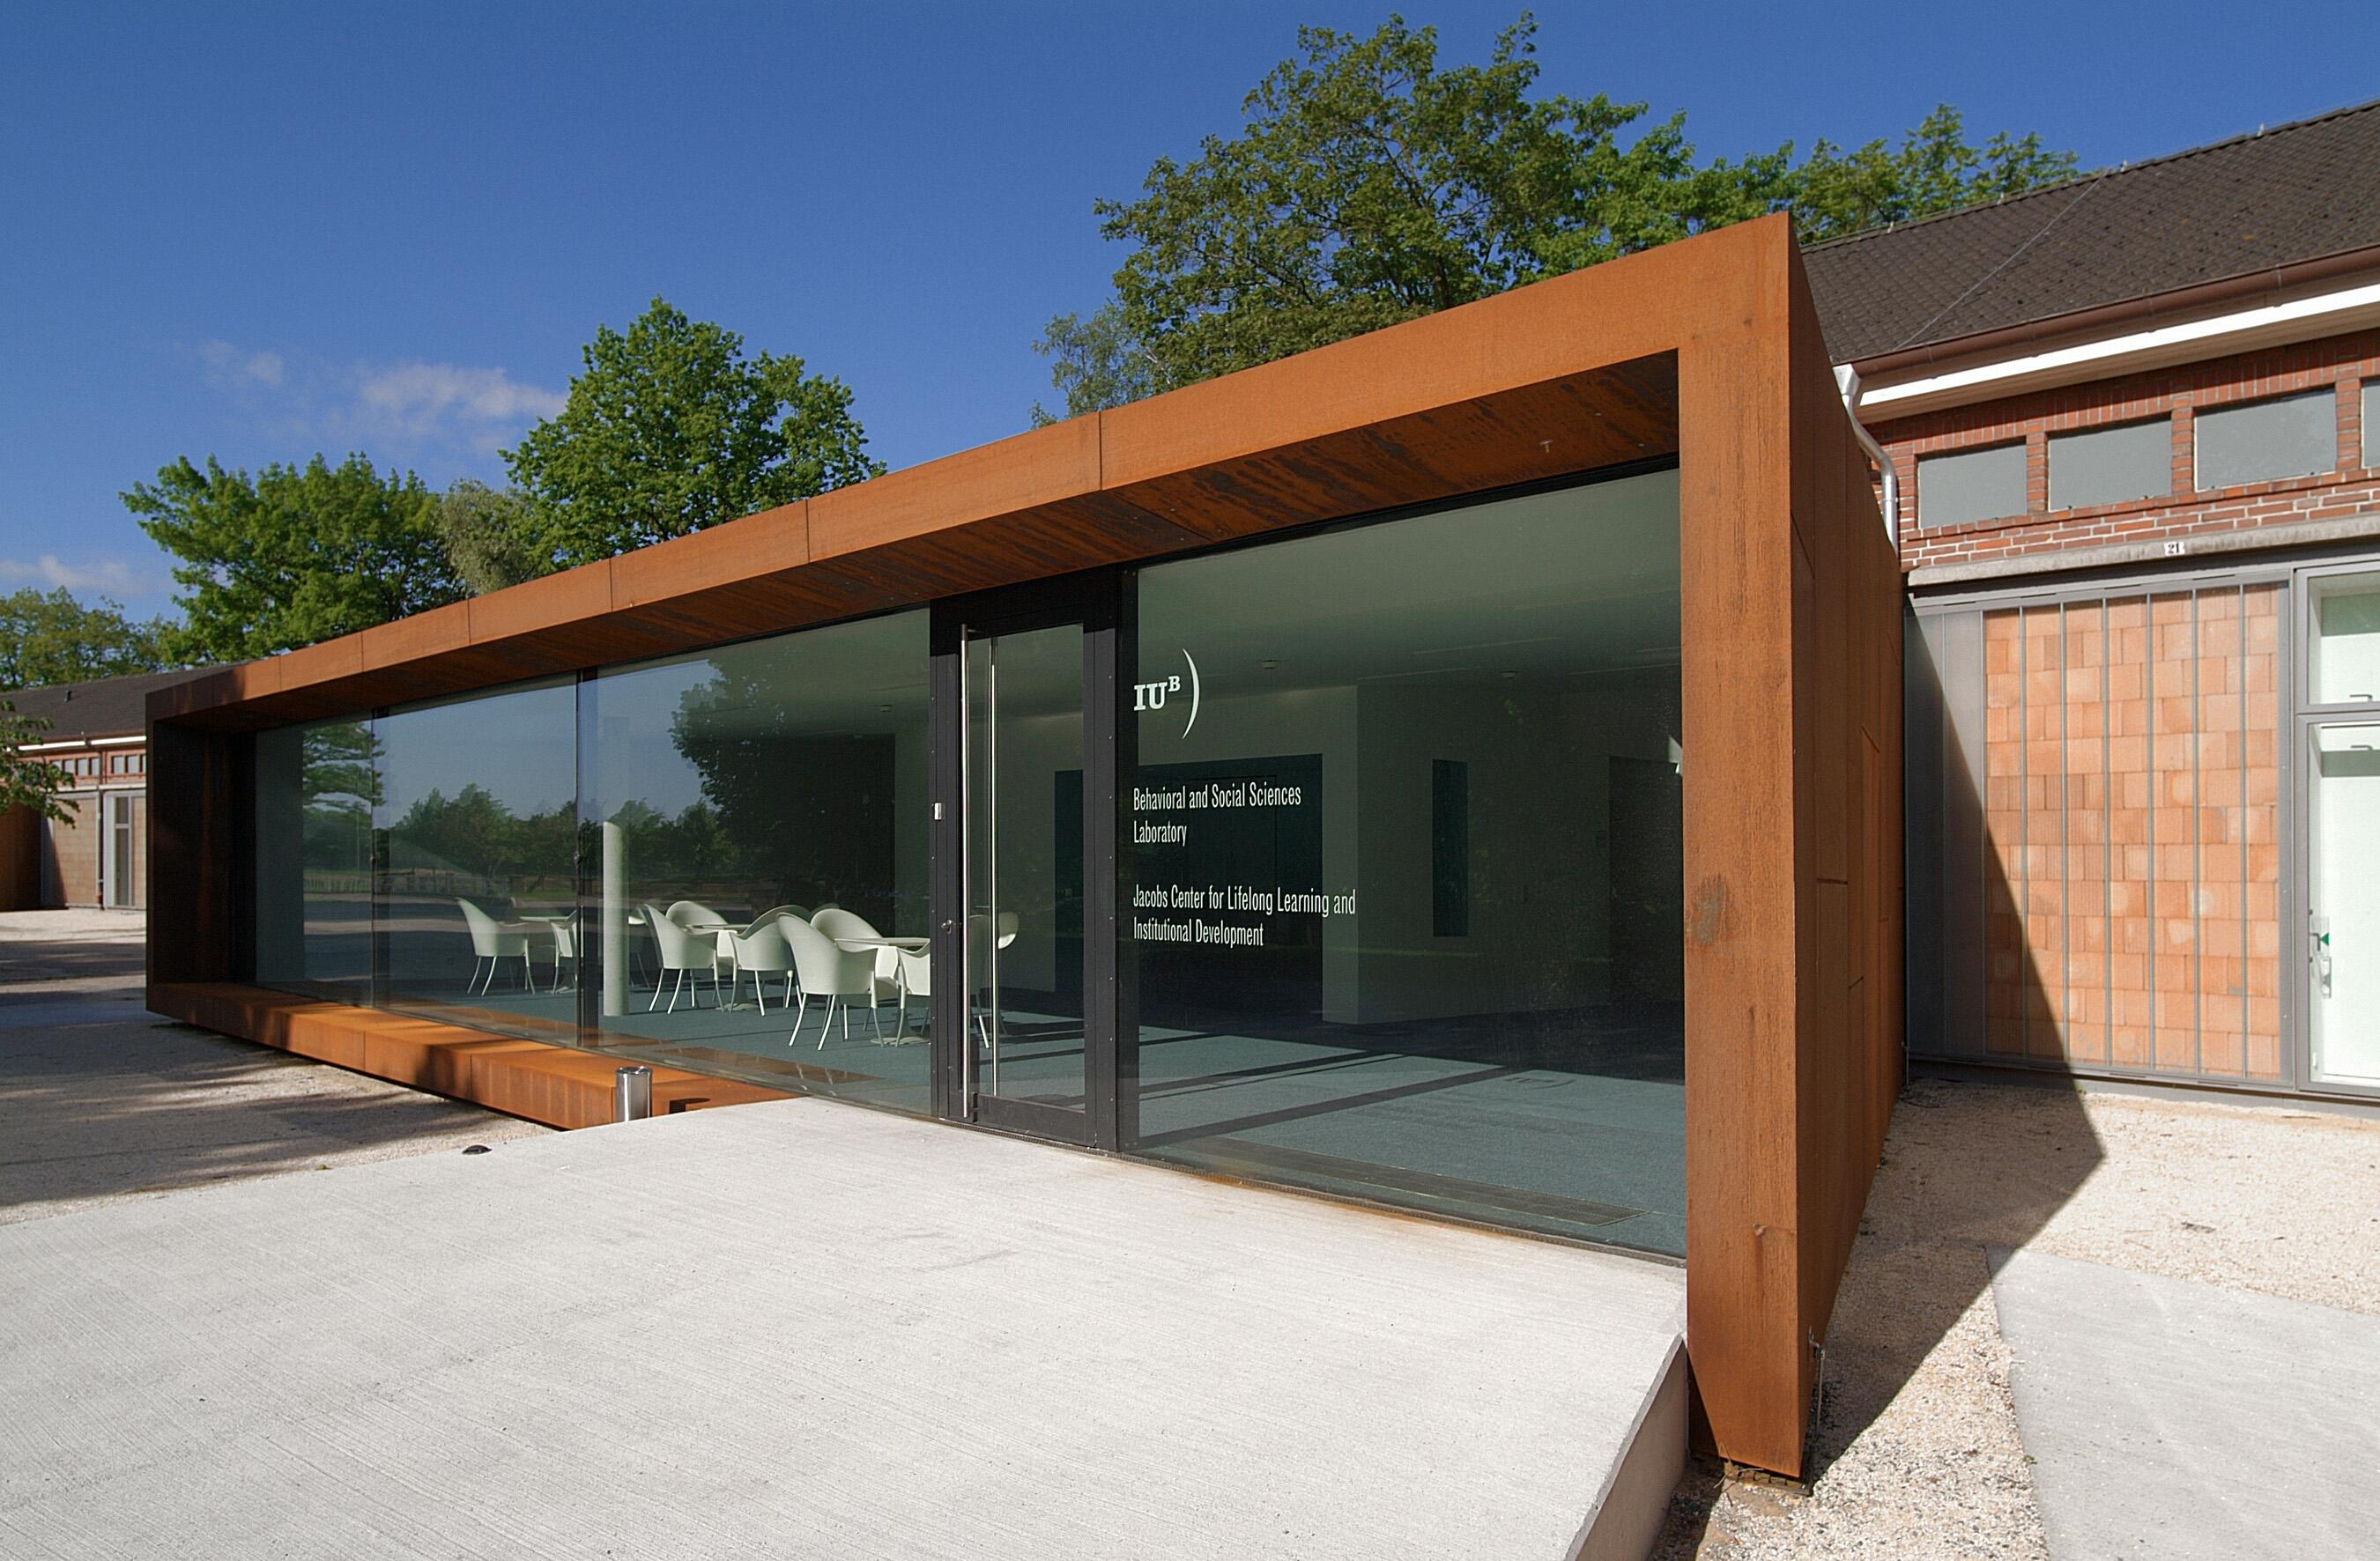
\includegraphics[width=0.5\textwidth,height=5cm]{photo2.jpg}
	\end{center}
\end{figure}


\cleardoublepage

\newpage
\section{Grants 2007/2008} \shorttitle{Grants 2007/2008}

\begin{itemize}

\item Bremen International Graduate School of the Social Sciences \textit{BIGSSS"}, Project in cooperation with the University Bremen and the SHSS (Co-PI: U. M. Staudinger), German Excellence Initiative, DFG, (2008-2011). 

\item BMBF (PI: Staudinger et al.). Joint research project:\textit{ Effects of Matches/Mismatches between Aspects of Human and Social Capital, Corporate Strategy and Work Organization on the Physical and Mental Well-Being of Employees }(2007 - 2010).

\item Emmy Noether Research Group, part I (KU 1401/4-1), part II (KU 1401/4-2), and part III (KU 1401/4-3) funded by the DFG, (PI: B.M. Kudielka) \textit{Stress and burnout - Integration of work psychological and psychobiological research methods for the assessment of differential stress patterns in chronic work stress }(2004 - 2009).

\item IRTG International Research Training Group ('Internationales Graduiertenkolleg') of Trier (Germany) and Leiden (The Netherlands) (GRH 1389/1); funded by the DFG (B.M. Kudielka was one out of 11 Co-Applicants (German part)) \textit{Psychoneuroendocrinology of stress: from molecules and genes to affect and cognition} (2006 - 2010).

\item Leopoldina (PI: U. M. Staudinger) \textit{Joint Academy Group: Aging in Germany}(2006-2009).

\item Robert Bosch Foundation (PIs: C. Voelcker-Rehage, B. Godde, U. M. Staudinger): \textit{Old Age on the Move} (2006-2009).

\item Volkswagen Foundation (PIs: B. Godde, K. Sch�mann, U. M. Staudinger) \textit{Job Mobility and Developmental Outcomes} (2008-2011).

\item Volkswagen Foundation (PI: C. Stamov Ro�nagel): \textit{Older workers' cognitive innovation resources} (2008-2011).

\item Volkswagen Foundation Initiative "Gesellschaftliche und kulturelle Herausforderungen Innovationsprozesse in Wirtschaft und Gesellschaft" (PIs: S. Voelpel and G. Van der Vegt): Proposal: \textit{The Effects of the Aging Workforce on the Innovation Process: A Large-Scale Study of Technology Intensive Companies} (2007-2010).

\end{itemize}
\cleardoublepage

\newpage
\section{Selected Knowledge Transfer Activities} \shorttitle{Selected Knowledge Transfer Activities}

\begin{itemize}

\item Executive Teaching for AutoUni in Wolfsburg by K. Sch�mann.

\item Executive Teaching for Schneider Electric, ThyssenKrupp AG, Volkswagen AG, by C. Stamov Ro�nagel.

\item Developing Executive Teaching Program for \textit{Next Generation Leadership Programme} in collaboration with TiasNimbas Business School (Tilburg, NL) by C. Stamov Ro�nagel, Course-Director.

\item Executive Teaching for Leadership Academy, Lower Saxony Penitentiary Service, German Society for Personnel Management (DGFP) by C. Stamov Ro�nagel.

\item Consulting Project (PI: K. Sch�mann): Evaluation of company-wide occupational health and safety trainings ENO/RNO Bremen.
ADECCO Institute (PI: K. Sch�mann and C. Rossnagel): Compendium on Lifelong Learning - Qualification Needs in the OECD - Analysis, Implementation and Policy Recommendations.

\item WISE Demographie Netzwerk (Companies: Deutsche Bahn, Deutsche Bank, EnBW, Lonza, Otto Group, VW) (PIs: S. Voelpel, C. Stamov Ro�nagel), (2007-2010).

\item Projekt Innovationsmanagement (Companies: EADS Astrium, KAEFER, Meyer Werft, Rheinmetall) (PI: S. Voelpel), (2007). 

\item Consulting Project (PI: C. Stamov Ro�nagel): \textit{An age-differentiated view on work and learning motivation at HeidelbergCement}. HeidelbergCement.

\item Consulting Project (PI: M. Schulz, C. Stamov Ro�nagel):\textit{ Evaluation of a learning competency training}. EnBW.

\end{itemize}
\cleardoublepage

\twocolumn
\newpage
\section{Awards and Honors Received by Members of the Jacobs Center} \shorttitle{Awards and Honors Received by Members of the Jacobs Center}

\textbf{Ben Godde / Claudia Voelcker-Rehage}

\begin{tabular}{l p{6cm}}
2007:	& Research Award from Sparkasse Bremen and Unifreunde Bremen to Ben Godde \& Claudia Voelcker-Rehage for cooperative projects between University Bremen and Jacobs University, together with Ekkehard K�stermann, Peter Erhard (both University Bremen), and Markus Ebke (Hospital Bremen-Center).
\end{tabular}

\textbf{Brigitte Kudielka/ Silja Bellingrath}

\begin{tabular}{l p{6cm}}
2008: & Biological Psychology Author Award for the Top cited Paper in 2006 and 2007 to Brigitte M. Kudielka and Clemens Kirschbaum for the paper "Sex differences in HPA axis responses to stress: a review", Volume 69/1 (2005).\\

2008:	&	Charlotte- und Karl-B�hler-Award 2008 of the German Society for Psychology (DGPs) to Brigitte M. Kudielka (endowed with \euro1000).\\

2008:	&	Young Investigator Award 2008 of the International Society of Psychoneuroendocrinology (ISPNE), to Silja Bellingrath, doctoral student in the Emmy-Noether Project (Principal Investigator: Brigitte M. Kudielka).\\

2007:	&	Scholar Award to Silja Bellingrath, doctoral student in the Emmy-Noether Project (Principal Investigator: Brigitte M. Kudielka) of the American Psychosomatic Society (APS).\\

2007:	&	Press Release Invitation for abstract: \textit{'Dysregulations of the HPA-axis and increased allostatic load in job-related chronic stress: A link to burnout and exhaustion in school teachers?'} authored by Bellingrath S., Hellhammer D.H., Kudielka B.M. at the 2007 Annual Meeting of the American Psychosomatic Society (APS).\\

\end{tabular}

\textbf{Ursula M. Staudinger}

\begin{tabular}{l p{6cm}}
2008-2010: & President German Psychological Society (DGPs)\\

2007-2013: & Vice President of the National Academy of Sciences Leopoldina\\
\end{tabular}

\paragraph{}

\textbf{Sven Voelpel}

\begin{tabular}{l p{6cm}}
2007: &	Nomination for the \textit{SMS Best Conference Paper for Practice Implications Award}. [Zhao, C.L., Han, Z. \& Voelpel, S. (2007). \textit{Meeting the environmental challenges: Strategies against counterfeiters in China}. 27th SMS Annual International Conference, October 14-17, 2007, San Diego, California, USA].\\
2007:	& Sven Voelpel: Nr. 5 in most read \textit{Organization Studies} articles [Nonaka, I., von Krogh, G., \& Voelpel, S. (2006). Organizational knowledge creation theory: Evolutionary paths and future advances. \textit{Organization Studies}, 27(8), 1179-1208.]\\
2007:	& Sven Voepel: Long Range Planning: Editor's 10 Excellent Articles List, 2007 [Beer, M., Voelpel, S., Leibold, M., \& Tekie, E. (2005). Strategic management as organizational learning: Developing fit and alignment through a disciplined process. \textit{Long Range Planning}, 38(5), 445-465.]
\end{tabular}
\cleardoublepage


\newpage
\onecolumn
\section{PhD Degrees}
\shorttitle{PhD Degrees}

\paragraph{2006} D\"orner, Jessica: ``A Self-Concept Measure of Personality Growth: Self-Concept Maturity (SCM). Development, Validation, and Age Effects''

Dissertation Committee: Prof. Dr. Ursula M. Staudinger (supervisor, IUB), Prof. Dr. Alexandra Freund (University of Zurich), Prof. Dr. Manfred Diehl (University of Florida, USA), Prof. Dr. Ulrich K\"uhnen (IUB), Prof. Dr. Britta Renner (IUB)

\paragraph{2006} Kessler, Eva-Marie: ``Intergenerational Relations as Facilitative Developmental Context'' 

Dissertation Committee: Prof. Dr. Ursula M. Staudinger (supervisor, IUB), Prof. Dr. Ute Kunzmann (IUB), Prof. Dr. Werner Greve (University of Hildesheim), Prof. Dr. Klaus Boehnke (IUB)

\paragraph{2005} Mickler, Charlotte: ``Self-related wisdom: Validation and age effects of a new measure of personal maturity'' 

Dissertation Committee: Prof. Dr. Ursula M. Staudinger (supervisor, IUB), Prof. Dr. Ute Kunzmann (IUB), Prof. Dr. Sigrun-Heide Filipp (University of Trier), Prof. Dr. Margrit Schreier (IUB)



\cleardoublepage

\newpage
\onecolumn
\section{Faculty} \shorttitle{Faculty}

\begin{tabular}{ll}
Dr. Godde, Benjamin	& Professor of Human Performance and Neuroscience\\
& \\
Dr. Kunzmann, Ute			& Professor of Psychology\\
& \\
Dr. Renner, Britta		&	Professor of Psychology\\
& \\
Dr. Rossnagel, Christian	&	Professor of Organizational Behavior (since 09/2006) \\
& \\
Dr. Sch\"omann, Klaus		&	Professor of Sociology\\
& \\
Dr. Schwender, Clemens	&	Professor of Communication Science\\
& \\
Dr. Staudinger, Ursula M.	&	Professor of Psychology\\
& \\
Dr. Voelpel, Sven			& Professor of Business Administration
\end{tabular}

\cleardoublepage

\newpage
\onecolumn
\section{Graduate Students and Postdoctoral Fellows} \shorttitle{Graduate Students and Postdoctoral Fellows}


\begin{tabular}{l p{12cm}}

Baron, Stefan &	Graduate Student (Sociology, since 04/2007).\\[6pt]
Bellingrath, Silja &	Postdoctoral Fellow (Health Psychology, since 10/2008).\\[6pt]
Biemann, Torsten	&	Postdoctoral Fellow (Business Administration,	since 09/2007).\\[6pt]
Bittner, Jennifer &	Postdoctoral Fellow (Organizational Behavior, since 12/2008).\\[6pt]
Bowen, Catherine &	Graduate Student (Psychology, since 04/2007).\\[6pt]
Dolge, Katja	& Graduate Student (Neuroscience, since 08/2008).\\[6pt]
Eckhoff, Robert	& Graduate Student (Business Administration, 	since 10/2007).\\[6pt]
Fasang, Anette &	Graduate Student (Sociology, until 08/2008).\\[6pt]
Feuerhahn, Nicolas	& Graduate Student (Health Psychology, since 	06/2008).\\[6pt]
Geerdes, Sara-Izabella	& Graduate Student (Sociology).\\[6pt]
Heidemeier, Heike	& Postdoctoral Fellow (Psychology).\\[6pt]
Isichenko, Polina	& Graduate Student (Business Administration).\\[6pt]
Kearney, Eric	& Postdoctoral Fellow (Business Administration, 	since 10/2007).\\ [6pt]
Korff, J�rg	& Graduate Student (Business Administration, 	since 08/2007).\\[6pt]
Licklederer, Claudia	& Graduate Student (Business Administration, 	since 07/2008).\\[6pt]
M�hlig-Versen, & Andrea	Graduate Student (Psychology, until 07/2008).\\[6pt]
Noack, Martin	& Graduate Student (Psychology).\\[6pt]
Noethen, Daniela	& Graduate Student (Business Administration, 	since 04/2007).\\[6pt]
Oeberst, Andries	& Graduate Student (Psychology).\\[6pt]
Otto, Siegmar	& Graduate Student (until 04/2007).\\[6pt]
Panzer, Martina	& Graduate Student (Psychology).\\[6pt]
Richter, David	& Graduate Student (Psychology).\\[6pt]
Sauer, Anne	& Graduate Student (Business Administration, 	since 10/2008).\\[6pt]
Schaffer, Stefan	& Graduate Student (Business Administration, 	since 11/2007).\\[6pt]
Schelkes, Daniel	& Graduate Student (Sociology, since 04/2008).\\[6pt]
Schulz, Melanie	& Graduate Student (Organizational Behavior).\\[6pt]
Speckmann, Katharina &	Graduate Student (Business Administration,	since 05/2008).\\[6pt]
Tekie, Eden &	Graduate Student (Business Administration).\\[6pt]
Trautmann, Mireille	& Postdoctoral Fellow (Neuroscience, since 12/2008).\\[6pt]
Zhao, Chunli &	Graduate Student (Business Administration).\\[6pt]

\end{tabular}

	

\cleardoublepage

\onecolumn
\newpage
\section{Where Have Our Researchers Gone?} \shorttitle{Where Have Our Researchers Gone?}

\paragraph{}
\paragraph{}

\begin{tabular}{l p{12cm}}
\textbf{Faculty} & \\
Kunzmann, Ute	& University of Leipzig	\\
Renner, Britta	& University of Constance\\
Schwender, Clemens	& University of�Management and�Communication 	Potsdam�(FH)\\
 & \\
\textbf{Postdoc} & \\
Han, Zheng	& University of St. Gallen\\
Kessler, Eva-Maria	& University of Heidelberg\\
 & \\
\textbf{ PhD}& \\
D�rner, Jessica &	University of Trier\\
Fasang, Anette	& Yale University, Postdoctoral Fellow\\
Mickler, Charlotte	& Humboldt University Berlin\\
M�hlig-Versen, Andrea	& University of Bremen, Research Associate\\
Otto, Siegmar	& Institute for Ecological Economy Research, 	Berlin, Research Associate\\
Streb, Chris	& University of Groningen, Assistant Professor\\
\end{tabular}
\cleardoublepage

\twocolumn
\newpage
\section{Visiting Scholars at the Jacobs Center} \shorttitle{Visiting Scholars at the Jacobs Center}


$$ $$
\textit{Prof. Dr. Nicola Baumann} (Department of Psychology, University of Trier, Presentation: "How do we grow? Personal growth through affect regulation").
$$ $$
\textit{Prof. Dr. Hans-Peter Blossfeld} (Holds the Chair of Sociology I and is the Director of the \href{http://www.ifb.bayern.de/}{Staatsinstitut f�r Familienforschung at Bamberg University}).
$$ $$
\textit{Prof. Dr. Andreas Diekmann} (Professor of Sociology, ETH Zurich, Presentation: 'Social Cooperation, Results from Experimental Game Theory').
$$ $$
\textit{Dr. Werner Eichhorst} (Institute for the Study of Labor (IZA), Bonn, Presentation: 'From Transfers to Training').
$$ $$
\textit{Prof. Dr. Michael Falkenstein} (Leiter der Projektgruppe "Altern und ZNS-Ver�nderungen", Institut f�r Arbeitsphysiologie (IfADo), Technische Universit�t Dortmund).
$$ $$
\textit{Denis Gerstorf, Ph.D.} (Assistant Professor of Human Development at the Department of Human Development and Family Studies, The Pennsylvania State University, State College (Held a lecture in July at Jacobs Center)).
$$ $$
\textit{Dr. Daniel Gr�hn} (FPSE-Psychology, University of Geneva, Presentation: 'The Positive and the Negative Side of Older Adults' Memory: Age-Related Differences in Remembering Emotional Information').
$$ $$
\textit{Prof. Dr. Thomas M. Hess }(Department of Psychology, North Carolina State University, NC, USA, Presentation: 'A Social Cognitive Approach to Understanding Aging and Decision Making: Affective, Motivational, and Experiential Influences').
$$ $$
\textit{Prof. Dr. Herbert Heuer }(Leibniz Research Center for Working Environment and Human Factors, Institute for work physiology, University of Dortmund, Presentation: 'Adaptation to Visuo-motor Rotations of Different Magnitude in Younger and Older Adults').
$$ $$
\textit{Prof. Dr. Johannes Huinink }(Professor f�r Soziologie mit Schwerpunkt "Theorie und Empirie der Sozialstruktur" am Institut f�r empirische und angewandte Soziologie der Universit�t Bremen).
$$ $$
\textit{Prof. Dr. Michael H�ther} (Honorary Professor at the European Business School, Director, Institut der deutschen Wirtschaft K�ln, Presentation: 'Intergenerational Justice and Economic Growth - A Challenge for Economic Policy').
$$ $$
\textit{Prof. Dr. J�rgen Kocka }(Chair for the History of the Industrial World at the Free University of Berlin, Presentation: 'Chances and Challenges of Aging Societies').
$$ $$
\textit{Prof. Dr. Gisela Labouvie-Vief }(Professor of Social-Emotional Development, University of Geneva, Switzerland, Presentation: 'Dynamic Emotion-Cognition Relations in Adulthood').
$$ $$
\textit{Prof. Dr. Marius Leibold }(Department of Business Management, Stellenbosch University, South Africa).
$$ $$
\textit{Prof. Dr. Pawel Lewicki} (Professor of Psychology, Psychology Department, University of Tulsa). 
$$ $$
\textit{Dr. Dr. Talat Mahmood} (Social Science Research Center Berlin (WZB); Berlin, Germany).
$$ $$
\textit{Prof. Dr. Karl Ulrich Mayer} (Professor of Sociology and Director of the \href{http://www.yale.edu/ciqle/}{Center for Research on Inequalities and the Life Course} (CIQLE) at Yale University, Presentation: 'New Directions in Life Course Research').
$$ $$
\textit{Prof. Dr. Franz J. Neyer} (Professor of Lifespan Development, University of Vechta, Presentation: 'Personality Development and Relationship Development').
$$ $$
\textit{Prof. Dr. Lars Nyberg} (Professor of Neuroscience, Ume? University, Sweden, Presentation: 'Memory and Executive Deficits in Relation to Fronto-Striatal Functioning').  
$$ $$
\textit{Prof. Dr. Ernst Poeppel} (Vorstand des Instituts f�r Medizinische Psychologie (IMP) der LMU M�nchen. Gesch�ftsf�hrender Vorstand des Humanwissenschaftlichen Zentrums (HWZ) der LMU M�nchen; Institute�of Medical Psychology, LMU Munich, Presentation: 'Fifty years and beyond: Too old to learn something new?').
$$ $$
\textit{Nilam Ram, Ph.D.} (Assistant Professor, Department of Human Development and Family Studies, The Pennsylvania State University, (Held a lecture in July at Jacobs Center)).
$$ $$
\textit{Prof. Dr. Patricia Reuter-Lorenz} (Professor of Psychology, University of Michigan, Ann Arbor, Presentation: 'Neuro-cognitive Aging and the Compensation Hypothesis').
$$ $$
\textit{Prof. Dr. Ram�n Rico} (Department of Social Psychology and Methodology, Faculty of Psychology, Universidad Aut�noma de Madrid). 
$$ $$
\textit{Prof. Dr. Klaus Rothermund }(Chair of General Psychology, Institut f�r Psychologie, Friedrich-Schiller-Universit�t Jena).
$$ $$
\textit{Prof. Dr. Georg Schrey�gg} (Professor of Organization and Leadership, Free University of Berlin, Presentation: 'Characteristics and Relevance of Knowledge-Intensive Firms').
$$ $$
\textit{Dr. Antje Stange} (Visiting�Scientist,�Adult Development Lab, Georgia�Institute�of�Technology,�School�of�Psychology, Atlanta, Presentation: 'Explaining Others' Behavior: When do Old and Younger People differ in their Social Judgments?').
$$ $$
\textit{Prof. Dr. J�rgen Wegge }(Professor of Industrial and Organizational Psychology, Technical University of Dresden, Presentation: 'The Aging Workforce: Problems and Chances with Respect to Effective Team Work').
$$ $$
\textit{Prof. Dr. Reinhold Wei�} (Deputy President and Head of Research of the Federal Institute for Vocational Education and Training (BIBB), Presentation: 'From Formal Training to a New Learning Culture: Trends and Challenges of Lifelong Learning').it{Prof. Dr. Sherry L. Willis} (Professor of Human Development, Pennsylvania State University, Presentation: 'Midlife: Risks and Resources').
$$ $$
\textit{Prof. Dr. Sherry L. Willis} (Professor of Human Development, Pennsylvania State University, Presentation: 'Midlife: Risks and Resources').
$$ $$
\textit{Dr. Gerben S. Van der Vegt }(Professor of Work and Organizational Psychology, Department of Management and Organization, University of Groningen, NL , Presentation: 'When and Why does Power Asymmetry Affect Team Performance?').
$$ $$
\textit{Prof. Dr. James W. Vaupel} (Director, Max Planck International Research Network on Aging, Professor of Demography, Max Planck Institute for Demographic Research, Rostock, Presentation: 'Remarkable Plasticity of Longevity - Policy Challenge of Population Aging').

\cleardoublepage

\onecolumn
\newpage
\section{JCLL Fact Sheets} \shorttitle{JCLL Fact Sheets}

\textbf{Development of Grants}

\begin{figure}[htbp]
	\begin{center}
		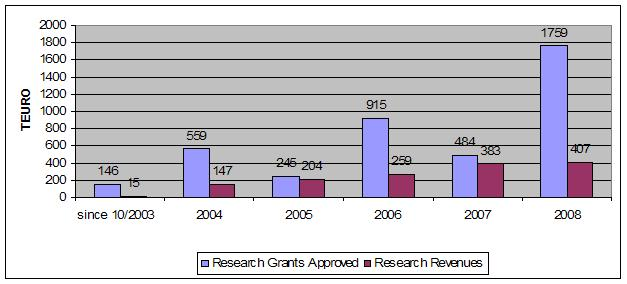
\includegraphics[width=1\textwidth,height=7.5cm]{photo3.jpg}
		\caption{ JCLL Revenues Research Grants 2003 - 2008 }
	\end{center}
\end{figure}
$$ $$
\textbf{Development of Publications}

\begin{figure}[htbp]
	\begin{center}
		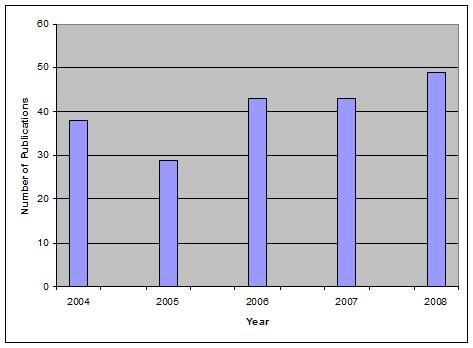
\includegraphics[width=0.7\textwidth,height=6.5cm]{photo4.jpg}
		\caption{Number of peer-reviewed articles, chapter in handbooks/encyclopedias, chapters in edited volumes, monographs, edited volumes, articles in popular science and other kinds of publications}
	\end{center}
\end{figure}

$$ $$
\paragraph{}
\textbf{Development of Staff}

\begin{figure}[htbp]

		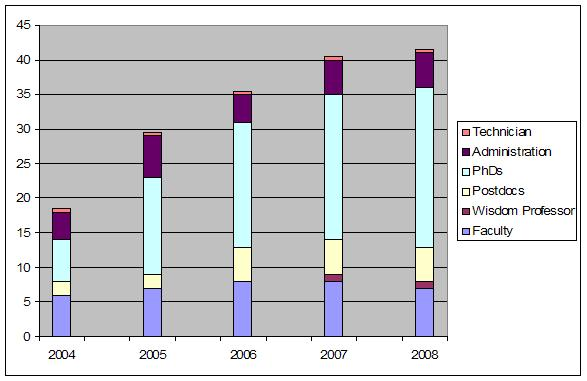
\includegraphics[width=1.0\textwidth,height=8cm]{photo5.jpg}
		\caption{Development of Personnel at the JCLL}

\end{figure}
\cleardoublepage

\onecolumn
\newpage
\section{Impressum} \shorttitle{Impressum}
$$ $$
\textit{Executive Editor}


Prof. Dr. Ursula M. Staudinger


Dean, Jacobs Center on Lifelong Learning and Institutional Development
$$ $$
\textit{Production Editor} and Editor


Dr. Krystin Zigan
$$ $$
\textit{Editors}


Prof. Dr. Ben Godde (Human Performance and Neuroscience)


Prof. Dr. Brigitte Kudielka (Health Psychology)


Prof. Dr. Klaus Sch�mann (Sociology)


Prof. Dr. Christian Stamov Ro�nagel (Organizational Behavior)


Prof. Dr. Ursula M. Staudinger (Psychology)


Dr. Claudia Voelcker-Rehage (Human Performance)


Prof. Dr. Sven Voelpel (Business Administration)
$$ $$
Cover Pictures: Department of Corporate Communications, Jacobs University Bremen



\end{document}
%------------ Into Dean ---------------------------------------------------------------
  %\input{xxx}
\cleardoublepage
% Each chapter starts on a right page
\ 

%
%
\subsubsection{Cellular and Wireless Communications}
\label{Haas1} \index{Haas, Harald}

\paragraph{Research Team}
Harald Haas (Professor), Rami Abu-Alhiga (PhD Student), Zubin
Bharucha (PhD Student), Hany Elgala (PhD Student), Ellina Foutekova
(PhD Student), Birendra Ghimire (PhD Student), Dennis Kolyuzhnov
(PhD Student),  Raed Youself Mesleh (PhD Student), Abdurazak Mudesir
(PhD Student), Hrishikesh Venkataraman (PhD Student), Sinan
Sinanovic (Research Associate), Peter Omiyi (Postdoc), Mostafa
Afgani (Research Engineer), Sudharasan Ganesan (Graduate Student)\\

Research in Cellular and Wireless Communications is geared towards
new technologies. Particular focus is  on the development and the
interaction of key air-interface building blocks \newpage

\begin{myitemize}
\item multicarrier transmission (in particular OFDM (Orthogonal Frequency Division
Multiplexing)
\item duplexing techniques (in particular time division duplexing
(TDD))
\item multiple-input multiple-output (MIMO) techniques
\item wireless ad hoc systems
\item medium access control (MAC) algorithms
\item multiple access and scheduling techniques
\item dynamic channel assignment (DCA) algorithms
\item mobile positioning
\item visible light communication.
\end{myitemize}

\myparagraph{Highlights} \emph{Spatial Modulation.} Spatial
modulation (SM) is a new and patented multiple antenna transmission
approach for wireless systems that increases the spectral efficiency
(number of bits transmitted per Hz bandwidth) by utilizing the
transmit antenna number as an implicit source of information. A
block of information bits is mapped to an information symbol and a
transmit antenna number. As a consequence, at any given time instant
only a single antenna of the antenna array is transmitting signal
power. The actual block of information bits determines which antenna
is active at a particular time instant. As a result, inter-channel
interference (ICI) at the receiver input and the need to synchronize
the transmit antennas are completely avoided. Simple receiver
algorithms such as maximum receive ratio combining (MRRC) can be
used to retrieve the information bits. The performance and the
receiver complexity of SM and V-BLAST (Vertical-Bell Labs Layered
Space-Time) algorithm in flat fading channels are compared. V-BLAST
applies zero forcing detection based optimum ordering, nulling and
successive interference cancellation. The basic principle of SM is
depicted in Fig.~\ref{smexmpl}, and results of the comparison with
state-of-the-art V-BLAST are shown in Fig.~\ref{fig55}.
\begin{figure}[!htb]\centering
  \centerline{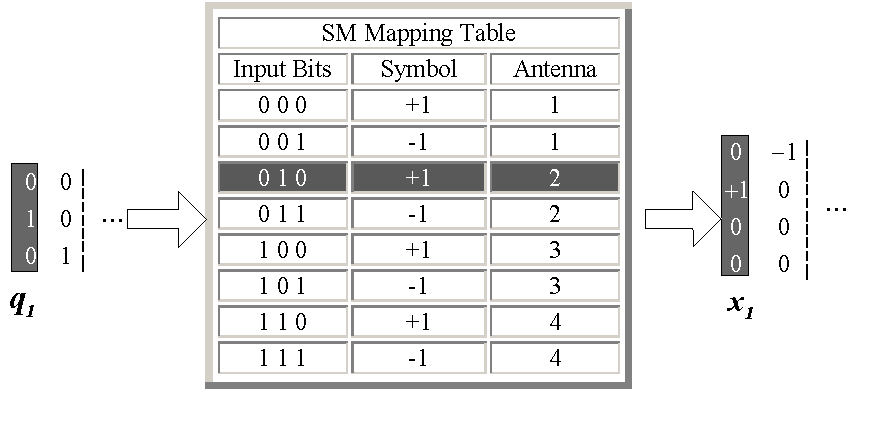
\includegraphics[width=8cm]{haas_1.pdf}}
  \caption{3bits/symbol spatial modulation mapping table using binary phase shift keying (BPSK)
    and four transmit antennas} \label{smexmpl}
\end{figure}
\begin{figure}[!!htp]\centering
  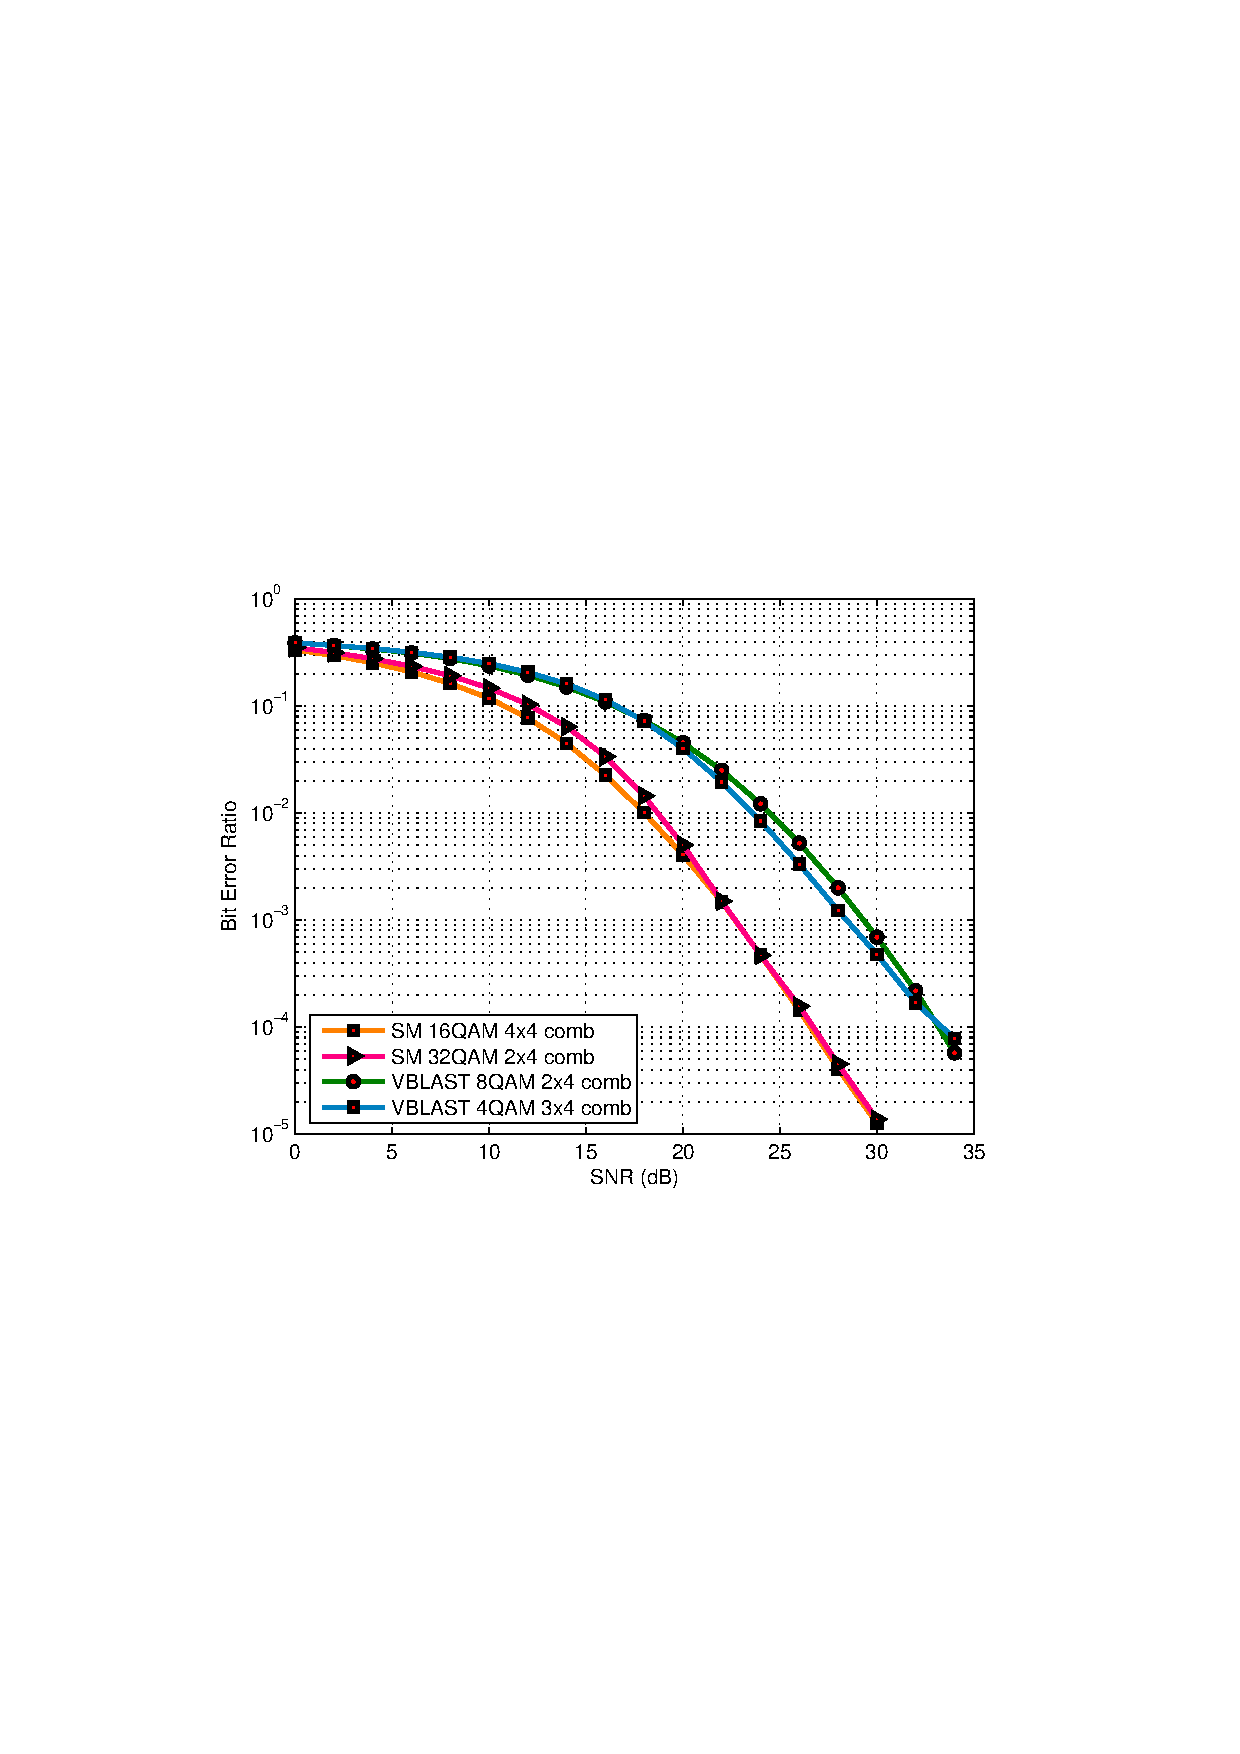
\includegraphics[width=8cm]{haas_2.pdf}\\
  \caption{Bit error performance as a function of signal-to-noise ratio (SNR) for state-of-the-art V-BLAST and novel SM.}
  \label{fig55}
\end{figure}
From the results it can be found that the performance gains are
significant. In both schemes the same number of bit per unit
bandwidth are transmitted (for fair comparison), but with SM the bit
error performance is reduced considerably. For example, at an SNR of
20dB a 10-fold reduction in the BER is observed.

\emph{Dynamic Resource Allocation.} In this work a fully
decentralized interference avoidance algorithm to manage
interference in an \emph{ad hoc} wireless network, applicable to
wireless sensor networks, is developed and analyzed. Fig.~\ref{dca}
depicts a randomly chosen distribution of transmitting (Tx) and
receiving (Rx) nodes. The new algorithm, called \emph{busy tone
interference tolerance signaling}, is of low complexity and is very
easy to implement. It is based on different functions to set the
busy tone signal power dependent on the level of tolerable
interference, and their performance is compared with a special case
of a fixed power system which provides maximum capacity assuming
equal transmit powers. Results show that an appropriately chosen
function for setting the busy-tone can lead to gains in capacity
using very little power. This power efficiency advantage is quite
significant, implying that battery life of units can be extended
while providing a similar capacity than a fixed power system.
\begin{figure}[!!htp]
 \centering
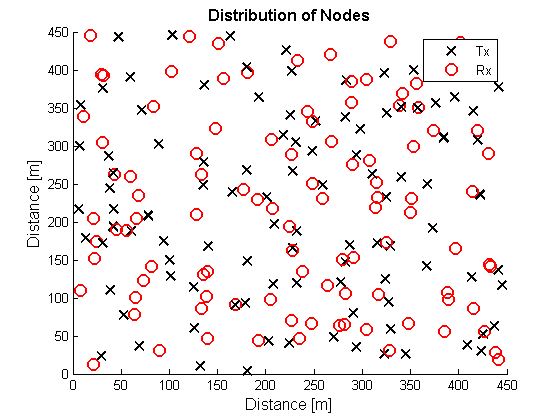
\includegraphics[width=8cm]{haas_3.png}\\
\caption{Random distribution of nodes in an \emph{ad hoc} wireless network}
\label{dca}
\end{figure}

%\null Harald Haas is also involved in ``Signal Processing''
%(Section~\ref{Haas1}).

%\newpage
\paragraph{Organization}
% list the (research) events you have organized, if any,
\begin{enumerate}
    \item Member of Technical Program Committee of and session chair
          at \emph{IEEE International Conference on Personal, Indoor \& Mobile Radio Communications} -- PIMRC 2006
    \item Member of Technical Program Committee of \emph{International IEEE Conference on Vehicular Technology} -- VTC 2006
\end{enumerate}

\paragraph{Collaborations}
\begin{enumerate}
\item {\sl The University of Edinburgh, UK}\\
  Prof. S. McLaughlin\\
  Joint project with industrial partner on \emph{Hybrid Cellular and Multihop Wireless
    Networks}
\end{enumerate}

\newpage
\paragraph{Grants}
% list the running grants in 2005, if none have been received, please delete this
% subsection.
\begin{enumerate}
    \item Funded by industry partner,
      \emph{Cellular TDD-OFDM (Time division duplex - orthogonal frequency
          division multiplexing)},  June 2004 - July 2005


    \item Funding by industry partner and University of Edinburgh, \emph{Hybrid Cellular and Multihop Wireless
    Networks},  July 2005 - July 2006

    \item Funded by industry partner, \emph{Link Adaptation and Scheduling in Cellular
    Systems},  March 2005 - February 2008

    \item Funded by Bremen T.I.M.E program funded by BIS
    Bremerhaven, \emph{Mobile Positioning (MPos)} in collaboration with MobilTec GmbH and supported by
     T-Mobile,  June 2006 - September 2009

    \item Funded by DFG Schwerpunktprogram TakeOFDM, \emph{DCA Algorithms and MAC Protocols for COFDM Based Cellular and
     Ad hoc Systems Using Carrier Sensing Time Division Multiple Access
     (CSTDMA)},  October 2004 - September 2006

\end{enumerate}

\paragraph{Patents}
% list the grants you have received in 2005, if none have been received, please delete this
% subsection.
\begin{enumerate}
\item Four new patent applications submitted
\item Three previously submitted patents got granted in 2006
\end{enumerate}

\paragraph{Awards, Prizes}
\begin{enumerate}
\item Nominated for the Chinese 111 Program -- Guest Academic Talents Programme for the Development of University Disciplines in China
\item Invited Talk at the University of Mondragon (Spain)
%    \item Honorary Fellowship of Edinburgh University
%    \item Invited to Institute for Digital Communications (IDCOM) at the University of
%          Edinburgh on \emph{Vodafone Fellowship on Communications}
    %\item Invited speaker at \emph{International Next Generation Wireless Network Workshop},
     %     Edinburgh/Scotland
\end{enumerate}

%\paragraph{Publications}
% list the publications of 2005 (also accepted and in press), if none have been received, please delete this
% subsection. Enter the publications into the SES publications database at
% http://kwarc.eecs.iu-bremen.de/ses-pubs/index.php and only reference them here.

 
\nocite{ah06_vis_light}
\nocite{bh06_ped_dead_reck}
\nocite{hnona06_iamac}
\nocite{vh06_thru_cap}
\nocite{cvh06_freq_syn}
\nocite{feh06_semi_analytic}
\nocite{fagvh06_sch_CDMA}
\nocite{jhm06_adhoc_tdd_underlay}
\nocite{oha06_tsalloc_insotdd}
\nocite{mhay06_spatialmod}
\nocite{asilomar06}
\nocite{chinacom06}
\nocite{tdd_book}
\nocite{oha07}
 

 
%\begin{bibunit}[hplain]
\begin{thebibliography}{10}

\bibitem{ah06_vis_light}
M.~Afgani and H.~Haas.
\newblock Visible light communication using {OFDM}.
\newblock In {\em Proceedings of the 2nd International Conference on Testbeds
  and Research Infrastructures for the Development of Networks and Communities
  (Trident 2006)}, Barcelona, Spain, March 01-06 2006.

\bibitem{bh06_ped_dead_reck}
S.~Beauregard and H.~Haas.
\newblock "{Pedestrian Dead Reckoning (PDR) and GPS for Indoor Positioning}".
\newblock In {\em Proceedings of 3rd Workshop on Positioning, Navigation and
  Communication ({WPNC}'06)}, Hannover, Germany, March 16 2006.

\bibitem{cvh06_freq_syn}
S.~Chaudhury, H.~Venkataraman, and H.~Haas.
\newblock "{Uplink Capacity Comparison of Non-Perfect Frequency Synchronised
  Cellular OFDM Systems}".
\newblock In {\em Proceedings of International Wireless Communications and
  Mobile Computing Conference ({IWCMC} 2006)}, Vancouver (Canada), July 3-6
  2006.

\bibitem{fagvh06_sch_CDMA}
E.~Foutekova, P.~Agyapong, B.~Ghimire, H.~Venkataraman, and H.~Haas.
\newblock "{Scheduling in Cellular TDD-CDMA Networks}".
\newblock In {\em Proceedings of the International Vehicular Technology
  Conference ({VTC}) 2006-Fall}, Montreal, Canada, September 25-28 2006. IEEE.

\bibitem{feh06_semi_analytic}
E.~Foutekova, C.~Evers, and H.~Haas.
\newblock "{Semi-Analytical Derivation of Interference in TDD-CDMA Systems
  Employing Random Time Slot Hopping (RTSH)}".
\newblock In {\em Proceedings of the International Vehicular Technology
  Conference ({VTC}) 2006-Fall}, Montreal, Canada, September 25-28 2006. IEEE.

\bibitem{asilomar06}
S.~Ganesan and H.~Haas.
\newblock "{On the Performance of Spatial Modulation OFDM}".
\newblock In {\em "{Asilomar Conference on Signals, Systems, and Computers}"},
  Monterey, CA, USA, October 30 -- November 1 2006. IEEE.

\bibitem{hnona06_iamac}
H.~Haas, V.~D. Nguyen, P.~Omiyi, N.~H. Nedev, and G.~Auer.
\newblock "{Interference Aware Medium Access in Cellular OFDMA/TDD Network}".
\newblock In {\em Proceedings of International Conference on Communications
  ({ICC} 2006)}, Istanbul, Turkey, June 11-15 2006. IEEE.

\bibitem{tdd_book}
H.~Harald and S.~McLaughlin, editors.
\newblock {\em "{Next Generation Mobile Access Technologies: Implementing
  TDD}"}.
\newblock Cambridge University Press, Spring 2007.

\bibitem{jhm06_adhoc_tdd_underlay}
P.~Jain, H.~Haas, and S.~McLaughlin.
\newblock "{Capacity Enhancement using Ad Hoc Pico-Cells and TDD Underlay}".
\newblock In {\em Proceedings of the 17th International Symposium on Personal,
  Indoor and Mobile Radio Communications ({PIMRC} 2006)}, page~5, Helsinki,
  Finland, September 11-14 2006. IEEE.

\bibitem{mhay06_spatialmod}
R.~Mesleh, H.~Haas, C.~C. Ahn, and S.~Yun.
\newblock "{Spatial Modulation -- OFDM}".
\newblock In {\em Proceedings of the International {OFDM} Workshop}, Hamburg,
  Germany, August 30-31 2006.

\bibitem{chinacom06}
R.~Mesleh, H.~Haas, C.~Wook Ahn, and S.~Yun.
\newblock "{Spatial Modulation -- A New Low Complexity Spectral Efficiency
  Enhancing Technique}".
\newblock In {\em "{ChinaCOM 2006}"}, Beijing, China, October 25 -- 27 2006.
  IEEE.

\bibitem{oha06_tsalloc_insotdd}
P.~Omiyi, H.~Haas, and G.~Auer.
\newblock "{Analysis of Intercellular Timeslot Allocation in Self-Organising
  TDD Cellular Mobile Systems}".
\newblock In {\em Proceedings of the 17th International Symposium on Personal,
  Indoor and Mobile Radio Communications ({PIMRC} 2006)}, page 5 pages on CD
  ROM, Helsinki, Finland, September 11-14 2006. IEEE.

\bibitem{vh06_thru_cap}
H.~Venkataraman and H.~Haas.
\newblock "{Throughput Capacity for 2-Hop Hybrid Cellular Networks}".
\newblock In {\em Proceedings of 6th Scandinavian Workshop on Wireless Ad-hoc
  Networks ({ADHOC} '06)}, Stockholm (Sweden), May 3-4 2006.

\end{thebibliography}
\end{bibunit}
%\subsubsection{Digital Transmission Methods and Coding}
\label{ict:cns:henkel} \index{Henkel, Werner}

\paragraph{Research Team}
Werner Henkel (Professor), Fangning Hu (PhD Student), Neele von Deetzen (PhD
Student), Khaled Shawky Hassan (PhD Student), Apirath Limmanee (PhD Student)\\

We currently concentrate on iterative decoding and unequal error protection in
coding and physical transport. In iterative decoding, we study the convergence
behavior and properties of analog Turbo-like codes and the possible design of
Turbo and LDPC codes for unequal error protection (UEP). In the design of UEP
codes, we especially cooperate with ENSEA, France, and Lule\aa\ University,
Sweden. UEP is also the goal in our multicarrier research, where we design
bit-allocation algorithms that allow for easy realization of different
protection classes in an arbitrary way. UEP will be a must for current and
especially future triple-play data services to different devices at varying
channel qualities.

The analog codes have a strong relation to signal processing. Regarding
practical applications of such codes, we especially look into the correction
of impulse-noise and clipping effects. There, the most important task is to
determine statistical properties that allow for easy erasure marking, which
would support further decoding steps, analog and digital.

We further started a project on data transmission using ultrasound signals. We
currently design lab experiments to deliver data for later modeling of the
channel and disturbances.

%%% give a very short (150 words description of your research area)
%% Hint: this can be copied from the research areas document (../masterplan/research-areas)

\paragraph{Highlights}

The design of UEP Turbo codes by a pruning approach led us to a structure that
we named hybrid concatenation, a combination of outer parallel and inner
serial concatenation. The study of the decoding convergence with so-called EXIT
charts yielded the result that the area between the curves describing the
outer iterations depend on the number of inner iterations. This allows for
minimizing the decoding complexity by a scheduling with varying number of
iterations in the different decoding steps (see Fig.~\ref{fig:henkel_1}). The
pruning concept was also the starting point for our design of UEP LDPC codes
with an irregular check-node profile (pat. pending).

\begin{figure}[ht]
  \centering
  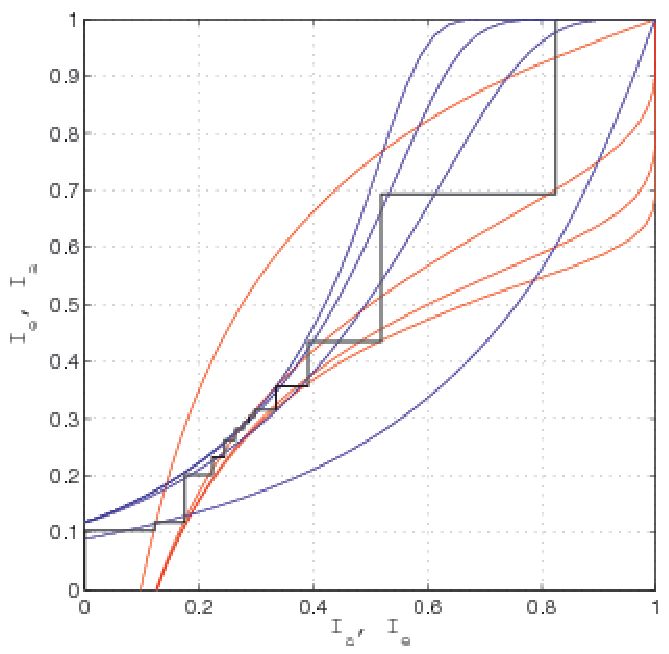
\includegraphics[width=7cm]{henkel_1}
 \caption{Convergence scheduling for hybrid concatenation}
%  \caption{Convergence scheduling for hybrid concatenation}
  \label{fig:henkel_1}
\end{figure}

In analog coding, we further improved the presentation of our proof that
Turbo-like decoding leads to a least-squares solution. We can now exactly
forecast the convergence limits for the stepsize and can also
modify it for every iteration to allow for very fast
convergence. For impulse-noise detection, we currently investigate new
statistical properties, e.g., the slope distribution, and correlation
approaches. This study will also close a gap in impulse-noise modeling
regarding the autocorrelation function of impulse noise.

By designing a new bit-allocation algorithm (pat. pending), following the
principles of an existing one by Chow, Cioffi, and Bingham, we can obtain UEP
properties in a very elegant way. It allows for an arbitrary number of
error-protection classes with arbitrary margins between them and an arbitrary
number of bits per class. Figure~\ref{fig:henkel_2} shows a resulting bit and
power allocation according to the channel SNRs, assuming three error protection
classes with a 3 dB separation.


\begin{figure}[ht]
  \centering
  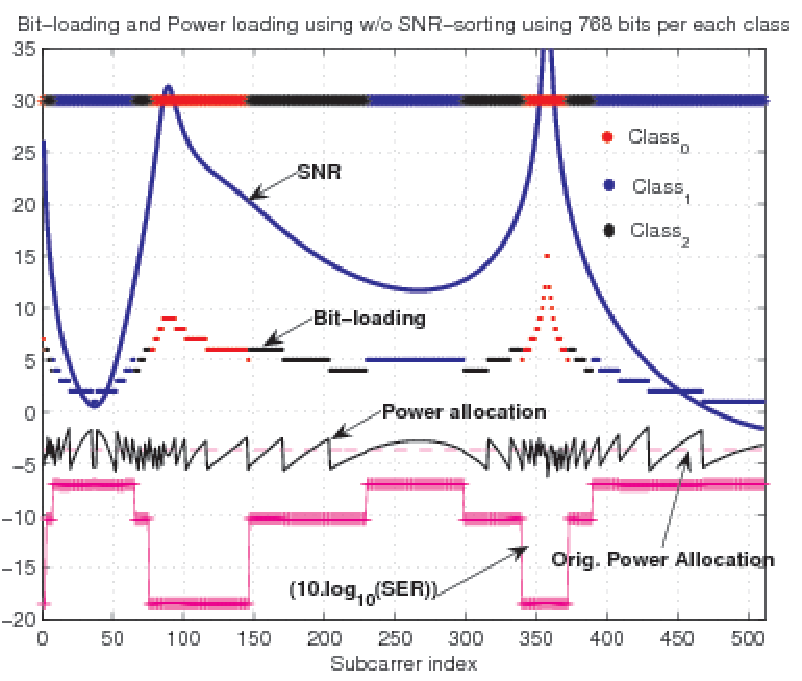
\includegraphics[width=7cm]{henkel_2}
  \caption{UEP bit and power allocation for three protection classes}
%  \caption{UEP bit and power allocation for three protection classes}
  \label{fig:henkel_2}
\end{figure}

\newpage
\paragraph{Organization}
% list the (research) events you have organized, if any,

\begin{enumerate}
\item Program Committee member of ICC 2006
\end{enumerate}

%\paragraph{Collaborations}
%\begin{enumerate}
%\item ...
%\item ...
%\item ...
%\end{enumerate}

\paragraph{Grants}
% list the running grants in 2005, if none have been received, please delete this
% subsection.
\begin{enumerate}
\item Funded by EU-IST STREP (FP 6), \emph{M-Pipe}, (October 2004
- March 2007)
\end{enumerate}

\paragraph{Patents}
\begin{enumerate}
\item  L. Sassatelli, W. Henkel, and D. Declercq. Check-Irregular LDPC Codes, Jan. 27
  2006. European Patent Application 06 100 979.1.
\item W. Henkel and K. Hassan. Unequal Error Protection Bit Loading for Multi-Carrier
  Transmission, Aug 30 2006. European Patent Application 06 119 771.1.
\end{enumerate}


%\paragraph{Publications}
% list the publications of 2005 (also accepted and in press), if none have been received, plese delete this
% subsection. Enter the publications into the SES publications database at
% http://kwarc.eecs.iu-bremen.de/ses-pubs/index.php and only reference them here.

%\begin{description}

%\item[Conference Proceedings]
  \nocite{Henkel_vDeetzen_IZS}
  \nocite{Hu_Henkel_Turbo}
  \nocite{Sassatelli_Henkel_Declercq_Turbo}
  \nocite{vDeetzen_Henkel_ISIT}
  \nocite{Henkel_Hassan_OFDM}
  \nocite{vDeetzen_ITG}
  \nocite{Hassan_Henkel_ITG}
%\item[Patents]
%  \nocite{Sassatelli_Henkel_Declercq_EP}
%  \nocite{Henkel_Hassan_EP}
%\end{description}

%%% Local Variables:
%%% mode: latex
%%% TeX-master: "report"
%%% End:

% \begin{bibunit}[hplain]\begin{thebibliography}{1}

\bibitem{Hassan_Henkel_ITG}
K.~Hassan and W.~Henkel.
\newblock {Unequal Error Protection Bit Loading in MIMO OFDM}.
\newblock In {\em ITG-Fachgruppe, 8. Sitzung}, Bremen, Oct. 6 2006.

\bibitem{Henkel_Hassan_OFDM}
W.~Henkel and K.~Hassan.
\newblock {OFDM (DMT) Bit and Power Loading for Unequal Error Protection}.
\newblock In {\em OFDM Workshop}, Hamburg, Aug 30-31 2006.

\bibitem{Henkel_vDeetzen_IZS}
W.~Henkel and N.~von Deetzen.
\newblock {Path Pruning for Unequal Error Protection Turbo Codes}.
\newblock In {\em 2006 International Z\"urich Seminar on Communications},
  Z\"urich, Switzerland, Feb. 22-24 2006.

\bibitem{Hu_Henkel_Turbo}
F.~Hu and W.~Henkel.
\newblock {A Geometric Description of the Iterative Least-Squares Decoding of
  Analog Block Codes}.
\newblock In {\em 4th International Symposium on Turbo Codes \& Related Topics
  in connection with the 6th International ITG-Conference on Source and Channel
  Coding}, Munich, April 4-7 2006.

\bibitem{Sassatelli_Henkel_Declercq_Turbo}
L.~Sassatelli, W.~Henkel, and D.~Declercq.
\newblock {Check-Irregular LDPC Codes for Unequal Error Protection under
  Iterative Decoding}.
\newblock In {\em 4th International Symposium on Turbo Codes \& Related Topics
  in connection with the 6th International ITG-Conference on Source and Channel
  Coding}, Munich, April 4-7 2006.

\bibitem{vDeetzen_ITG}
N.~von Deetzen.
\newblock {Decoder Scheduling of Hybrid (parallel/serial) Turbo Codes}.
\newblock In {\em ITG-Fachgruppe, 7. Sitzung}, Munich, May 22 2006.

\bibitem{vDeetzen_Henkel_ISIT}
N.~von Deetzen and W.~Henkel.
\newblock {Decoder Scheduling of Hybrid Turbo Codes}.
\newblock In {\em 2006 IEEE International Symposium on Information Theory (ISIT
  2006)}, Seattle, Washington, USA, July 9-14 2006.

\end{thebibliography}
\end{bibunit}

\onecolumn
\%input{Teaching}
%
 \newpage
\shorttitle{The School of Engineering and Science}
\section{The School of Engineering and Science}
\subsection{Administration}
\shorttitle{Administration of the School of Engineering and Science}
\begin{tabular}{ll}
Prof. Dr. Kramer, Bernhard &Vice President and Dean \\
 Dr. Allner, Anke
 & Director, Dean's Office \\ Schreiber, Angela  & Assistant to
the Dean \\ Buck, Iris  & Graduate Admission \\
 Dr. Frischholz, Svenja
& Graduate Student Affairs \\
 Knoop, Katja & Team Assistant to the
Faculty \\
 Manss, Sigrid  & Team Assistant to the Faculty \\
 Pankratz, Elke
&Team Assistant to the Faculty
\end{tabular}

\subsection{Advisory Board}
\begin{tabular}{ll}
  Prof. Dr. Andrew S. Douglas (Chair)  & Johns Hopkins University, Baltimore, MD \\
 Prof. Dr. med.
Hans-Jochen Heinze & Otto-von-Guericke-Universit�t, Magdeburg\\
Prof. Dr. Gotthilf Hempel & Bremen \\
 Prof. Dr. James L. Kinsey & William Marsh Rice University, Houston, TX\\
  Prof. Dr. Berrien Moore
III,  & University of New Hampshire \\ Prof. Dr. Heinz-Otto Peitgen
& MeVis, Bremen \\ Prof. Dr. Klaus Pinkau &M�nchen \\ Prof. Dr.
Manfred T. Reetz & Max-Planck-Institut f�r Kohlenforschung,
M�hlheim/Ruhr \\ Prof. Dr. Karl Wieghardt & Max-Planck-Institut f�r
Strahlenchemie, M�hlheim/Ruhr \\
\end{tabular}

\shorttitle{Faculty} \subsection{Faculty}
\begin{longtable}{ll}
Antoulas, Athanasios C., Ph.D.&Visiting Professor of Electrical Engineering  \\
Dr. Baier, Stephan& Visiting Lecturer in Mathematics \\
Dr. Bau, Michael& Associate Professor of Geosciences\\
Dr. Baumann, Peter& Associate Professor of Computer Science \\
Dr. Belov, Alexei& Visiting Professor of Mathematics \\
Dr. Bergholz, Werner& Professor of Electrical Engineering \\
Dr. Bijma, Jelle& Adjunct Professor of Marine Geosciences \\
& Alfred Wegener Institute for Polar and Marine Research \\
Dr. Birk, Andreas& Associate Professor of Computer Science  \\
Dr. Bode, Mathias& Lecturer of Electrical Engineering \\
Dr. Boetius, Antje& Associate Professor of Microbiology  \\
Dr. Brix, Klaudia& Professor of Cell Biology \\
Br\"uggen, Marcus, Ph.D.&Associate Professor of Astrophysics \\
Dr. Carpin, Stefano& Assistant Professor of Computer Science \\
Fern�ndez-Lahore, Marcelo, Ph.D.&Associate  Professor of Downstream-Processing \\
Dr. Fritz, J\"urgen& Assistant Professor of Biophysics \\
Dr. Gl\"ockner, Frank Oliver& Associate Professor of Bioinformatics  \\
& (joint appointment with the MPI for Marine Microbiology)\\
Haas, Harald, Ph.D.&Associate  Professor of Electrical Engineering \\
Dr. Haerendel, Gerhard& Distinguished Professor of Space Physics\\
Dr. Henkel, Werner& Professor of Electrical Engineering \\
Hilgetag, Claus C.,Ph.D.&Associate Professor of Neuroscience \\
Dr. H\"{u}tt, Marc-Thorsten& Associate Professor of Computational Systems Biology \\
Dr. Jaeger, Herbert& Associate Professor of Computational Science\\
Dr. Jeltsch, Albert& Professor of Biochemistry \\
Dr. Kaimanovich, Vadim& Professor of Mathematics \\
Dr. Khalili, Arzhang& Professor of Computational Science \\
& (joint appointment with the MPI for Marine Microbiology)\\
Dr. Kleinekath\"{o}fer, Ulrich& Associate Professor of Physics \\
Dr. Knipp, Dietmar& Assistant Professor of Electrical Engineering \\
Dr. K\"ohler, Angela& Adjunct Professor of Marine Biology \\
& Alfred Wegener Institute for Polar and Marine Research \\
Dr. Kohlhase, Michael& Professor of Computer Science \\
Kortz, Ulrich, Ph.D.&Associate Professor of Chemistry \\
Dr. Koschinsky-Fritsche, Andrea& Associate Professor of Geosciences \\
Dr. K\"uhl, Nicole& Research Instructor (Biochemistry \& Cell Biology) \\
Dr. Kuhnert, Nikolai& Associate Professor of Chemistry \\
Dr. Lerchl, Alexander& Professor of Biology \\
Dr.-Ing Linsen, Lars& Associate Professor of Computer Science and
Computational Science \\
Dr. L\"{o}we, Astrid& Research Assistant in Physics\\
Dr.-Ing Mahleko, Bendick& University Lecturer of Electrical
Engineering \\
Mallahi-Karai, Keivan, Ph.D.&Visiting Lecturer of Mathematics \\
Dr. Materny, Arnulf&  Professor of Chemical Physics  \\
Dr. Meyer-Ortmanns, Hildegard&  Professor of Physics  \\
Meyer-Rochow, V. Benno, Ph.D., D.Sc. &Professor of Biology  \\
Dr. Muskhelishvili, Georgi& Professor of Genetics \\
Dr. Nau, Werner& Professor of Chemistry \\
Nugent, Thomas, Ph.D.&Assistant Professor of Chemistry  \\
Oliver, Marcel, Ph.D.&Assistant Professor of Mathematics \\
Dr. Oswald, Peter& Professor of Mathematics \\
Dr. Penkov, Ivan& Professor of Mathematics \\
Pfander, G\"otz, Ph.D.&Assistant Professor of Mathematics \\
Richards, Ryan M., Ph.D.&Assistant Professor of Chemistry \\
Dr. Roccatano, Danilo& University Lecturer of Chemistry \\
Dr. Rosswog, Stephan& Assistant Professor of Astrophysics \\
% \end{longtable}
% \newpage
% \begin{longtable}{ll}
Schleicher, Dierk, Ph.D.&Professor of Mathematics  \\
Dr. Sch\"onw�lder, J\"urgen& Associate Professor of Computer
Science \\
Schupp, Peter, Ph.D.&Professor of Physics  \\
Dr. Schwaneberg, Ulrich& Associate Professor of Biochemical Engineering \\
Springer, Sebastian, D.Phil. &Assistant Professor of Biochemistry and Cell Biology\\
Dr. Stamerjohanns, Heinrich& Research Assistant, Head of Computer Science Lab \\
Dr. Stoll, Michael& Associate Professor of Mathematics \\
Dr. Styrkas, Konstantin& Visiting Assistant Professor of Mathematics \\
Tautz, Stefan, Ph.D.&Associate Professor of Physics \\
Dr. Thomsen, Laurenz& Professor of Geosciences \\
Dr. Ullrich, Matthias& Professor of Microbiology \\
Unnithan, Vikram, Ph.D.&Assistant Professor of Geoscience \\
Dr. Vogt, Joachim& Associate Professor of Physics \\
Dr. Wagner, Veit&  Associate Professor of Physics \\
Wallace, Jon, Ph.D.&Assistant Professor of Electrical Engineering \\
Wells, Raymond O., Ph.D.&Distinguished Professor of Mathematics  \\
Dr. Welte, Dietrich& Adjunct Professor of Geosciences \\
Dr. Wiltshire, Karen Helen& Professor of Geoscience \\
Dr. Winterhalter, Mathias& Professor of Biophysics  \\
Dr. Zacharias, Martin& Associate Professor of Computational Biology \\
Zupanc, G\"unther K. H.,Ph.D.&Professor of Neurobiology       \\

\end{longtable}

\shorttitle{Staff} \subsection{Staff}
\begin{longtable}{ll}
Abu-Alhiga, Rami & Integrated PhD Student (Electrical Engineering)\\
Afgani, Mostafa & Research Associate (Electrical Engineering) \\
Al-Buloshi, Mohammed & Graduate Student (Biochemical Engineering)\\
Al-Karablieh, Nehaya & Graduate Student (Microbiology)\\
Al-Shbat, Shering & Integrated PhD Student (Computer Science)\\
Alexander, Brian & Graduate Student (Geology/Geochemistry)\\
%Dr. Allner, Anke-Maria & Director, Dean's Office \\
Bakirci, Huseyin & Graduate Student (Chemistry)\\
Dr. Balster, Torsten & Research Associate\\
Bassil, Bassem & Graduate Student (Nanomolecular Science)\\
Becker, Sandra & Lab Assistant (Biology)\\
Behnke, Torsten & Technician, Ocean Lab\\
Benor, Amare & Graduate Student (Electrical Engineering)\\
Berger, Michael & Graduate Student (Biochemistry)\\
Bharucha, Zubin & Integrated PhD Student (Electrical Engineering) \\
Binner, Sabine & Research Assistant (Biochemical Engineering)\\
Blanusa, Milan & Graduate Student (Biochemical Engineering)\\
Dr. Blohmann, Christian & Postdoctoral Fellow (Physics)\\
Borchert, Britta & Graduate Student (Biochemistry)\\
Braun, Yvonne & Research Associate/Graduate Student (Microbiology)\\
B\"{u}th, Heiko & Graduate Student (Cell Biology)\\
Burau, Claudia & Lab Assistant (Biochemistry)\\
Caballero Hern\'{a}ndez, Josefa & Graduate Student (Biochemical Engineering)\\
Cabrera, Rosa & Postdoctoral Fellow (Downstream Processing) \\
Chahar, Sanjay & Graduate Student (Biochemistry)\\
Chan, Kah-Yoong & Graduate Student (Electrical Engineering)\\
%                    \end{longtable}
%                   \newpage
%                   \begin{longtable}{ll}
Chonnaparamutt, Winai & Graduate Student (Computer Science)\\
Chubarova, Elena, Ph.D. & Postdoctoral Fellow (Chemistry) \\
Claus, Ute & Lab Assistant (Biochemistry) \\
Curusku, Jeremy & Research Associate (Computational Biology) \\
Dairpoosh, Farnoosh& Graduate Student (Biochemical Engineering) \\
Dammann, Frauke & IMO Assistant (Mathematics)\\
Dan, Marius & Graduate Student (Astrophysics) \\
de Jesus Mendes, Pedro Andr\'{e} & Graduate Student (Geosciences)\\
Dr. Dehnert, Manuel& Postdoctoral Fellow (Computational Systems Biology) \\
Dhayalan, Arunkumar & Graduate Student (Biochemistry)\\
Dickman, Michael, Ph.D. & Senior Research Associate (Chemistry)\\
Dinkel, Thomas & Graduate Student (Electrical Engineering) \\
Donfack, Patrice & Graduate Student (Chemical Physics) \\
Donnelly, Stephen & Postdoctoral Fellow (Mathematics) \\
Dunkhorst, Anna & Graduate Student (Cell Biology) \\
Ehlers, Birte-Marie & Graduate Student (Geosciences)\\
El-Sheshtawy, Hamdy & Graduate Student (Chemistry) \\
Elgala, Hany & Lab Assistant (Electrical Engineering) \\
%Dr. Frischholz, Svenja & Assistant (Administration Graduate Students)\\
Felden, Janine & Graduate Student (Marmic) \\
Fu, Yanzhe & Graduate Student (Geosciences) \\
Gama Saldago, Antonio & Research Associate (Neurobiology) \\
Garcia Gutierrez, Angelica & Graduate Student (Computer Science) \\
Garcia-Novoa, Rosa & Graduate Student (GeoOcean Dynamics)\\
Garstka, Malgorzata & Graduate Student (Biochemistry)\\
Gburek, Benedikt & Research Associate and Graduate Student (Physics) \\
Geberth, Daniel & Graduate Student (Computational Systems Biology) \\
Geertz, Marcel & Graduate Student (Biochemistry)\\
Dr. Gelessus, Achim & CLAMV Server Manager\\
Ghimire, Birendra & Graduate Student (Electrical Engineering) \\
Gobet, Angelique & Graduate Student (Marmic)\\
Ghosh, Abhijit & Graduate Student (Chemistry)\\
Grote, Karen & Technical Assistant (Biology)\\
Guimbretiere, Thomas & Graduate Student (Astrophysics) \\
Hanelt, Sharifah Nora & Research Associate (Geosciences) \\
Hassan, Khaled & Research Associate (Electrical Engineering)\\
Hassanin, Rasha & Graduate Student (Chemical Physics) \\
Hauschildt, Jakob & Graduate Student (Geophysics)\\
Dr. Helling, Robert & Research Associate (Physics)\\
Hennig, Andreas & Graduate Student (Chemistry) \\
Dr. Henze, Stina & Research Associate (Physics)\\
Hinsch, Karen & Graduate Student (Neuroscience)\\
Dr. Hoeft, Matthias & Postdoctoral Fellow (Astrophysics)\\
Hofbauer, Michael & Electronic Technician (Ocean Lab)\\
Holzapfel, Christine & Lab Assistant Chemistry\\
Hoppe, Arne & Graduate Student (Physics)\\
Hu, Fangning & Graduate Student (Electrical Engineering)\\
Dr. Hu, Jun-Cheng & Postdoctoral Fellow (Chemistry) \\
Hussain, Firasat & Graduate Student (Chemistry)\\
Ihle, Saskia & Graduate Student (Biochemical Engineering)\\
Ismail, Amal & Graduate Student (Chemistry)\\
Ivanovska, Tetyana & Graduate Student (Computer Science)\\
Jordans, Silvia & Graduate Student (Cell Biology)\\
Josuttis, Daniela & Lab Technician (Biochemical Engineering)\\
Jurkowski, Renata & Graduate Student and Research Associate (Biochemistry)\\
Jurkowski, Thomasz & Graduate Student (Biochemistry)\\
Kaffl, Alexandra & Graduate Student (Mathematics)\\
von der Kammer, Bernd& Lab Assistant Physics \\
Kannan, Srinivasaraghavan & Research Associate (Biology) \\
Dr. Karpen, Volker & Research Associate (Oceanography)\\
%\end{longtable} \newpage
%\begin{longtable}{ll}
Keithahn, Christian & Graduate Student (Biology)\\
Klepsch, Meike & Lab Assistant (Biochemistry and Cell Biology) \\
Klose, Melanie & Graduate Student (Biology) \\
%Knoop, Katja& Team Assistant to the Faculty \\
Kohlhase, Andrea & Guest (Computer Science)\\
Kolyuzhov, Dennis & Graduate Student (Electrical Engineering)\\
Konradi, Jakow & Graduate Student (Physics)\\
Kottmann, Renzo & Graduate Student (Marine Microbiology)\\
Kraynov, Alexander & Graduate Student (Chemistry)\\
Kronenberger, Astrid & Graduate Student (Physics)\\
Kurtev, Stoyan & Graduate Student (Neuroscience)\\
Dr. Laser, Heike & Postdoctoral Fellow (Biology)\\
Laskowski, Katja & Lab Assistant (Biochemistry \& Cell Biology)\\
Lau, Tin Fan Stanley & Graduate Student (Biology)\\
Laubner, Bastian & Integrated PhD Student (Mathematics) \\
Liebert, Kirsten & Research Associate, Graduate Student (Biochemistry)\\
Limmanee, Apirath & Graduate Student (Electrical Engineering)\\
Lindemann, Marcus & Graduate Student (Biochemical Engineering)\\
Dr. Linnenberg, Susanne & Research Assistant (Teaching Lab Physics)\\
Linow, Marina & Research Associate (Biochemical Engineering)\\
Lucosevicius, Mantas & Graduate Student (Computer Science)\\
Mal, Sibsankar & Graduate Student (Chemistry)\\
%Manss, Sigrid & Team Assistant to the Faculty\\
Marbler, Herwig & Research Associate (Geosciences)\\
Maurer, Sebastian & Graduate Student (Biochemistry)\\
Mavathur, Ramesh & Graduate Student (Biochemistry)\\
Mawick, Jule & Lab Assistant (Geoscience)\\
May, Andreas & Graduate Student (Biochemical Engineering)\\
Mayer, Kristina & Graduate Student (Cell Biology)\\
Mei\ss ner, Daniela & Technical Assistant (Biology)\\
Mesleh, Read & Graduate Student (Electrical Engineering)\\
Mishra, Monalisa & Graduate Student (Biology)\\
Moje, Annika & Lab Assistant (Geoscience) \\
Molchanov, Vladimir  & Graduate Student (Mathematics) \\
Momeu, Iuliana Carmen & Graduate Student (Biochemical Engineering)\\
Mudesir, Abdurazak & Graduate Student (Electrical Engineering)\\
M\"uller, Christine & Graduate Student (Computer Science)\\
M\"uller, Jan Steffen & Graduate Student (Mathematics)\\
M\"uller, Normen & Graduate Student (Computer Science) \\
M\"uller-Linow, Mark & Graduate Student (Computational Systems Biology)\\
Namboodiri, Vinu & Graduate Student (Chemical Physics)\\
Nazor, Jovanna & Graduate Student (Biochemical Engineering) \\
Neu, Florian & IRCCM/CLAMV Systems Administrator\\
Nour Abdel-Gawad Ahmed, Mohammed & Graduate Student (Computer Science)\\
Normann, Immanuel & Graduate Student (Computer Science)\\
Nsouli, Nadeen & Graduate Student (Chemistry) \\
Dr. Omiyi, Peter & Postdoctoral Fellow (Electrical Engineering)\\
Onaca, Ozana & Graduate Student (Biochemical Engineering)\\
Pagel, Uwe & Electrical Engineering \& Computer Science Technician\\
%Pankratz, Elke & Team Assistant to the Faculty\\
Pathak, Kaustubh, Ph.D. &Postdoctoral Fellow (Computer Science) \\
%                   \end{longtable} \\
%                   \newpage
%                   \begin{longtable}{ll}
Pereira Da Silva Gomes, Joana Filipa & Postdoctoral Fellow (Biophysics)\\
Pezeshki, Soroosh & Graduate Student and Research Associate (Physics)\\
Pfingsthorn, Max & Graduate Student (Computer Science)\\
Piedra-Garza, Luis & Graduate Student (Chemistry)\\
Poppescu, Traian & Graduate Student (Astrophysics)\\
Poppinga, Jann & Graduate Student (Computer Science)\\
Prabhakar, Rajendran & Graduate Student (Nanomolecular Science)\\
Praeg, Daniel, Ph.D. & Research Associate (Geosciences)\\
Prodanovic, Radivoje, Ph.D. & Postdoctoral Fellow (Biochemical Engineering)\\
Purser, Autun & Integrated PhD Student (Geosciences)\\
Qu, Hong & Graduate Student (Cell Biology)\\
Rabe, Florian & Graduate Student (Computer Science)\\
Radicchi, Filippo & Graduate Student (Physics)\\
Dr. Ragozin, Sergey & Postdoctoral Fellow (Biochemistry)\\
Rajendran, Raphael Samuel & Graduate Student (Neurosciences)\\
Dr. Ramaye, Yannic & Postdoctoral Fellow (Biophysics)\\
Rashkov, Peter & Graduate Student (Mathematics)\\
Rathert, Philipp & Graduate Student (Biochemistry)\\
Rehders, Maren & Lab Assistant (Biochemistry and Cell Biology)\\
Reicke, Markus & Lab Assistant (Chemistry)\\
Dr. R\"{o}diger, Elke & Research Associate (Astrophysics)\\
Rohde, Christian & Graduate Student (Biochemistry)\\
Rosenk\"{o}tter, Frank & Lab Assistant (Physics)\\
Rosenthal, Paul & Graduate Student (Computer Science)\\
R\"{u}ckert, Johannes & Graduate Student (Mathematics)\\
Rulli, Matteo & Graduate Student (Physics)\\
Sahoo, Harekrushna & Graduate Student (Chemistry)\\
Santillano, Daniel & Graduate Student (Marmic)\\
Scaria, Abraham & Graduate Student (Physics)\\
Dr.Sch\"{a}fer, Angela & Research Associate (IRCCM)\\
Dr. Schirmer, Thomas & Research Associate (Geosciences)\\
Schlickenrider, Martina & Research Associate (Biochemistry)\\
Schmidt, Katja & Graduate Student (Geoscience)\\
Schneewei{\ss}, Clemens & Research Associate (Biochemistry)\\
%Schreiber, Angela & Assistant to the Dean\\
Schr\"{o}der, Markus & Graduate Student and Research Associate (Physics)\\
Schwarzlose, Thomas & Research Assistant, Teaching Lab Chemistry\\
Dr. Schwarzpaul, Kristin & Research Associate (Biology)\\
Schwerdtfeger, Maike & Lab Assistant Biochemistry \\
Schwertfeger, S\"{o}ren & Graduate Student (Computer Science)\\
Shaik, Mona & Visiting Graduate Student (Electrical Engineering)\\
Sieker, Florian & Graduate Student (Bioinformatics)\\
Sharma, Praseh & Graduate Student (Geosciences)\\
Simon, Tatjana & Technical Assistant (Biology)\\
Dr. Solodukhin, Sergey N. & Senior Research Associate (Physics)\\
Dr. Sommer, Angela & Research Associate (Biology)\\
Dr. Soubatch, Serguei & Research Associate (Physics)\\
Sourly-Gopala, Divakara & Graduate Student (Chemistry)\\
Srivastava, Abhishek & Graduate Student (BioRec)\\
Stroehlein, Thomas & Animal Keeper\\
Suchopar, Andreas & Lab Assistant Chemistry \\
Tayakuniyil, Praveen & Graduate Student (Biochemistry)\\
Tee, Kang Lan & Graduate Student (Biochemical Engineering)\\
Temirov, Ruslan & Graduate Student (Nanomolecular Science)\\
Thomsen, Claudia & Research Associate (Oceanography) \\
% \end{longtable}
%                   \newpage
%                   \begin{longtable}{ll}
Thon, Michael & Graduate Student (Mathematics)\\
T\"{o}mmers, Stephanie & Graduate Student (Biochemical Engineering)\\
Tran, Ha Manh & Graduate Student (Computer Science)\\
Tran, Que-Tien & Graduate Student (Biophysics)\\
Tran, Van Long & Graduate Student (Computer Science)\\
Vennapusa, RamiReddy & Graduate Student (Biochemical Engineering)\\
Venkatraman, Hrishikesh & Graduate Student (Electrical Engineering)\\
Vilone, Daniele, Ph.D. & Postdoctoral Fellow (Physics)\\
Viergutz, Thomas & Marine Technology Engineer\\
von Deetzen, Neele & Graduate Student (Electrical Engineering)\\
Wagner, Hannes & Graduate Student (Geosciences)\\
Wakchaure, Vijay & Graduate Student (Chemistry)\\
Wecker, Patricia & Graduate Student (Microbiology)\\
Wellbrock, Ursula & Research Assistant (Biology)\\
Wensing, Annette & Graduate Student (Microbiology)\\
Wong, Tuck Seng & Graduate Student (Biochemical Engineering)\\
Wolters, Brit & Graduate Student (Cell Biology)\\
W\"{u}rdemann, Chris Andr\'{e} & Graduate Student (Genetics)\\
Yaneva, Rakina & Graduate Student (Cell Biology)\\
Yang, Mouyu & Graduate Student (Biology)\\
You, JiangJiang & Graduate Student (Astrophysics)\\
Dr. Yu, Jin & Postdoctoral Fellow (Neuroscience)\\
Zhang, YingYing & Graduate Student (Biochemistry)\\
Zhao, Mingjie, Ph.D. & Postdoctoral Fellow (Electrical Engineering)\\
Zhu, Ziwei & Graduate Student (Biochemical Engineering)\\
Dr. Zieger, Bertalan & Postdoctoral Fellow (Physics)\\
Dr. Zieger, Marina & Postdoctoral Fellow (Biology)\\
Dr. Zupanc, Marianne & Research Associate (Neurobiology)\\
%
%                      \end{longtable}
%                  \newpage
%\begin{longtable}{ll}

\end{longtable}
%\end{center}

\newpage
\shorttitle{ICTS Guests} \subsection{ICTS Guests} \label{ICTS}



\begin{longtable}{ll}
  Professor Dr.~Roland Benz &   Universit\"at
W\"urzburg, Germany
\\
Professor Dr.~Jan Bergstra&  University of Amsterdam, The Netherlands\\
Dr.~Andrey Bessonov& University of Sankt Petersburg, Russia\\
Dr.~S.M. Bezrukov&  National Institute of Health, Bethesda, USA\\
Dr. Georges Bouzerar&   Laboratoire Louis Nel, Grenoble, France\\
Dr. Henk Bruin&  University of Surrey, UK\\
Professor Dr.~Mark Burgess& University College Oslo, Norway\\
Professor Dr.~Val\'erie Cabuil&     Universit\'e Pierre et Marie
Curie, Paris, France\\
Dr.~Fabio Cavaliere& Universit\'a di Genova, Italy \\ Professor
Dr.~Shengbo Chen&      Institute of Geography and Natural
Resources, Beijing, PR China\\
Elizabeth Dan-Cohen&     University of California, Berkeley, USA\\
Professor Dr.~Gero Decher&      Institut Charles Sadron, Strasbourg,
France\\
Dr.~Martin Evans&        University of Edinburgh, UK\\
Dr.~Tom Fisher&      University of Cambridge, UK\\
Dr.~Claus F\"utterer&       Institut Marie Curie, Paris, France\\
Professor Dr.~Mariano Grasselli&     Universidad Nacional de
Quilmes,
Argentina\\
Dr.~Giovanni Indiveri&       University of Lecce, Italy\\
Professor Dr.~Dieter J\"ager&      Emory University, Atlanta, USA\\
Professor Dr.~Larry S. Liebovich&        Florida Atlantic
University,
USA\\
Professor Liviu Movileanu&      Syrakuse University, USA\\
Dr.~Sergei Nechaeev&     CNRS Orsay, France\\
Professor Dr.~Catherine O'Neill&     Columbia University, USA\\
Dr.~Marieke Postma&     NIKHEF, Amsterdam, The Netherlands\\
Dr.~Enrico Ramirez-Ruiz&    Institute of Advanced Studies,
Princeton, USA\\
Professor Dr.~Helmut Ringsdorf&      Universit\"at Mainz, Germany\\
Dr.~Karin R\"omisch&       University of Cambridge, UK\\
Lucile Sassatelli&       ENSEA-ETIS, Cergy-Pontoise, France\\
Professor Dr.~J\"urgen Schnack&        Universit\"at Osnabr\"uck,
Germany\\
Professor Dr.~Gerhard Schwarz&       Biozentrum Basel, Switzerland\\
Professor Dr.~Vera Serganova&       University of California,
Berkeley, USA\\
Professor Dr.~Nobuo Shimamoto&     National Institute of Genetics,
Mishima, Japan\\
Professor Dr.~Canan Tari&        Izmir Institute of Technology,
Turkey\\
Professor Dr.~Alexander Tikhomirov&  Yaroslavl State Pedagogical
University, Russia\\
Dr.~Andrew Travers&      Medical Research Council, Cambridge, UK\\
Dr.~Martin Weigt&        ISI Foundation, Torino, Italy\\
Professor Dr.~James Whisstock&      Monash University, Victoria,
Australia\\
Dr.~Wojtek Zakrzewski&   University of Durham, UK\\
Dr.~Michael Zaks&    Humboldt-Universit\"at Berlin, Germany\\
Professor Dr.~Gregg Zuckerman&   Yale University, USA.
\end{longtable}


\end {document}

